\chapter{Architecture des processeurs}
\label{chap:sota:materiel} \label{annexe:CHAPITRE_ARCHITECTURE} 


    \minitoc
    \glsresetall


L'objectif de cette annexe est de regrouper et présenter les principaux concepts techniques et technologiques qu'il a été nécessaire d'assimiler pour réaliser ce travail de thèse. En regroupant ces connaissances dans ce manuscrit, nous souhaitons faciliter le travail de futurs étudiants ou de futurs programmeurs souhaitant s'intéresser de plus près à la microarchitecture des processeurs. Pour cela, le chapitre regroupe les concepts étudiés en les empilant progressivement à la manière du modèle OSI \cite{day1983osi} :
\begin{itemize}
    \item Niveau 1 - Le circuit logique (\autoref{sec:logique})
    \item Niveau 2 - Les processeurs 
        \begin{itemize}
            \item L'architecture (\autoref{sec:micro})
            \item La hiérarchie mémoire (\autoref{sec:hierarchie})
        \end{itemize}
    \item Niveau 3 - Le système d'exploitation
        \begin{itemize}
            \item La mémoire virtuelle  (\autoref{sec:memoire_virtuelle})
        \end{itemize}
    %\item Niveau 4 - Les langages et compilateurs
\end{itemize}


    \iflong
        \section{Le circuit logique} \label{sec:logique}
%%%%%%%%%%%%%%%%%%%%%%%%%%%%%%%%%%%%%%%%%%%%%%%%%%%%%%%%%%%%%%%%%%%
%%%%%%%%%%%%%%%%%%%%%%%%%%%%%%%%%%%%%%%%%%%%%%%%%%%%%%%%%%%%%%%%%%%
Le niveau plus bas abordé dans cette annexe est celui des transistors qui sont les composants de bases de tout système électronique. 

\subsection{Les Transistors}
%%%%%%%%%%%%%%%%%%%%%%%%%%%%%%%%%%%%%%%%%%%%%%%%%%%%%%%%%%%%%%%%%%%
    Le premier transistor a été mis au point par des chercheurs des Laboratoires Bell en 1947 \cite{bardeen1948transistor}, dont la découverte avait été réalisée quelque années avant \cite{edgar1930method}. Ils apparaissent alors comme une révolution face aux tubes électroniques utilisés jusque là (plus rapide, plus léger et plus robuste). Un transistor est un composant électronique qui utilise trois bornes: la base, l’émetteur et le collecteur (voir \autoref{pic:transistor}). Le collecteur est relié au fil d’où vient la tension et correspond à la sortie du transistor. L’émetteur est lui relié à la masse (tension 0 volt). La base établie la connexion entre le connecteur et l'émetteur, en fonction de la tension qui lui est appliquée. En appliquant une tension faible à la base, le courant entre le collecteur et l’émetteur est possible. Sans aucune tension appliquée à la base, le passage du courant n’est pas possible. Pour les personnes non familières avec ces concepts électriques, une approche vulgarisée peut être utilisée \cite{JohnLeDuc2017}. Ainsi, le transistor se comporte comme un interrupteur binaire très rapide (basculement de l'ordre de $10^{-9}$ seconde).
    
    
    
    \begin{figure}[htbp]
        \centering
        \begin{subfigure}[b]{0.45\linewidth}\centering
            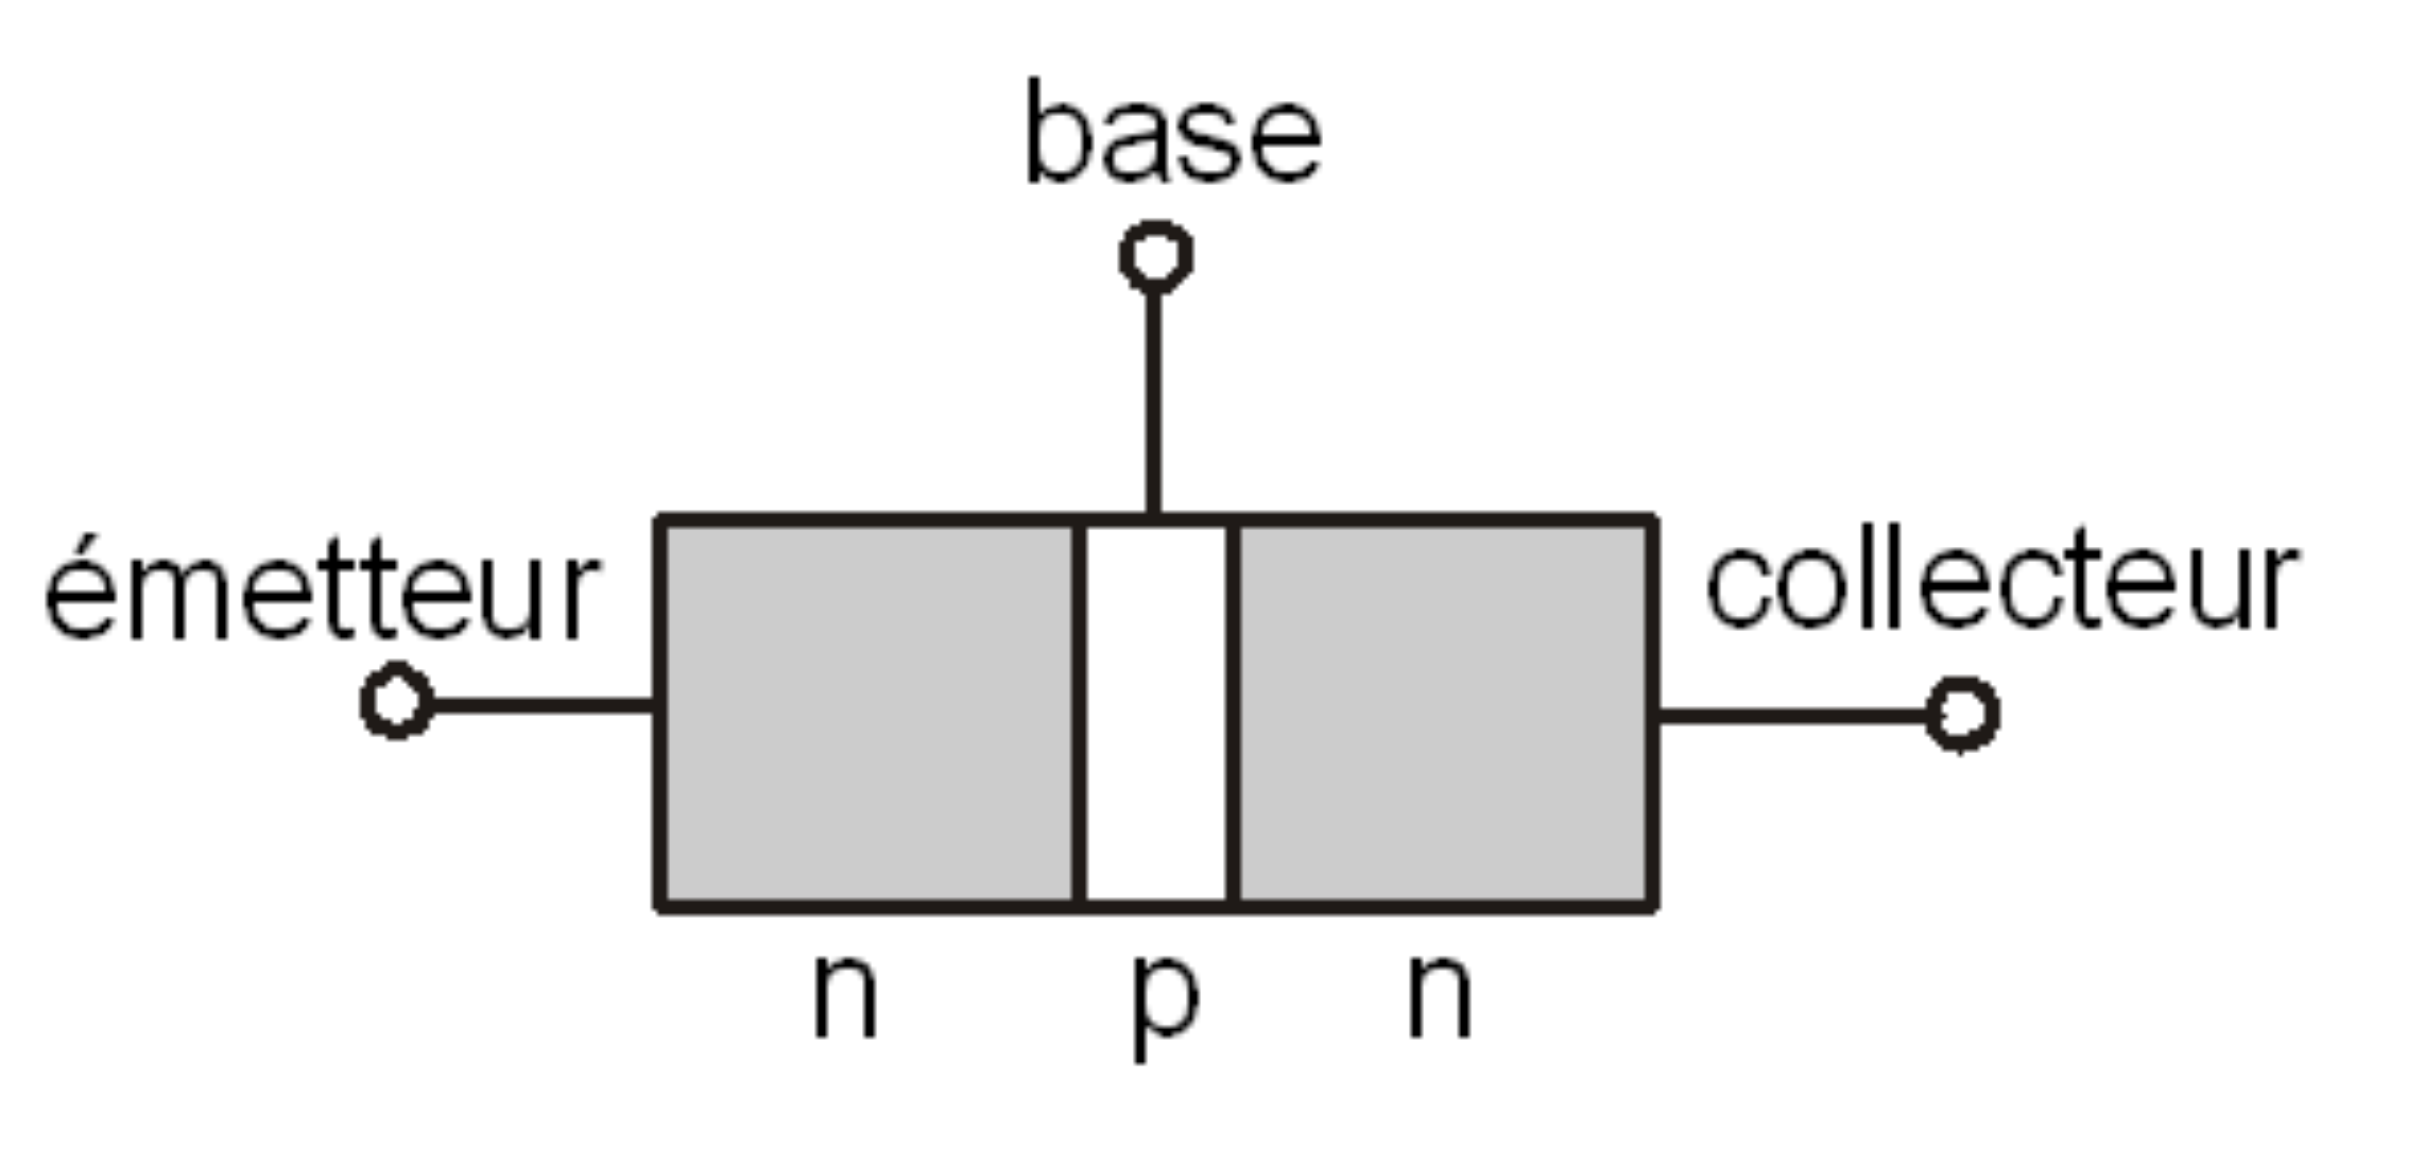
\includegraphics[width=\linewidth]{images/transistor.png}
            \caption{\label{pic:transistor} Schéma d'un transistor NPN \cite{GeraldHuguenin2018}}.
        \end{subfigure}
        ~ %add desired spacing between images, e. g. ~, \quad, \qquad, \hfill etc.
          %(or a blank line to force the subfigure onto a new line)
        \begin{subfigure}[b]{0.45\linewidth}\centering
            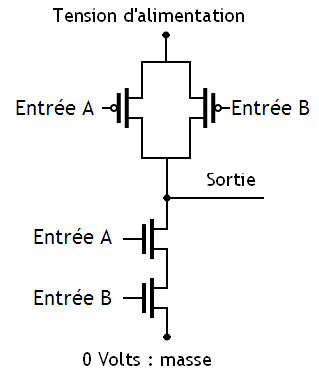
\includegraphics[width=0.5\linewidth]{images/processeur_porte_nand.png}
            \caption{\label{pic:processeur_porte_nand} Schéma électrique d'une porte \textit{NON-ET} réalisée à partir de 4 transistors \cite{Wikibooks2019PorteNand}}
        \end{subfigure}
        \caption{Un transistor est utilisé pour réaliser des portes complexes  }\label{pic:transistor_usage}
    \end{figure}




\subsection{Les portes logiques}
%%%%%%%%%%%%%%%%%%%%%%%%%%%%%%%%%%%%%%%%%%%%%%%%%%%%%%%%%%%%%%%%%%%
    
    Les portes logiques sont construites à partir de transistors et permettent l'exécution de différentes instructions ou la capacité de stocker une information (registres). Par exemple, en associant deux transistors inverseur en série on construit une porte NON-ET qui ne laisse passer le courant seulement lorsqu'aucune ou une des deux entrées a une tension (voir \autoref{pic:processeur_porte_nand})



    Une porte logique possède plusieurs entrées numériques qui peuvent être le résultat d'autres portes logiques (voir \autoref{pic:processeur_portes}). Les circuits les plus complexes sont en fait une cascade de milliers de portes logiques comme celles-ci. Il est aussi nécessaire de choisir la signification du passage ou non du courant et construire des portes ayant un « sens ». Il est courant d’utiliser les termes \verb|VRAI| ou \textit{1 logique} lorsque le courant circule et \verb|FAUX| ou \textit{0 logique} pour l’absence de tension.
    
    
    \begin{figure}
    \begin{subfigure}{.3\textwidth}
    \centering
    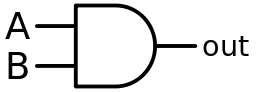
\includegraphics[width=0.80\linewidth]{images/processeur_porte_et.png}
    \caption{La porte \texttt{ET} ne laisse passer le courant seulement si les deux entrées sont \texttt{VRAI}}
    \end{subfigure}\hfill
    \begin{subfigure}{.3\textwidth}
    \centering
    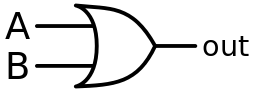
\includegraphics[width=0.80\linewidth]{images/processeur_porte_ou.png}
    \caption{La porte \texttt{OU} laisse passer le courant si au moins une des deux entrées est \texttt{VRAI}}
    \end{subfigure}\hfill
    \begin{subfigure}{.3\textwidth}
    \centering
    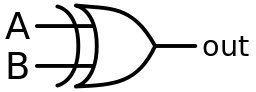
\includegraphics[width=0.80\linewidth]{images/processeur_porte_oux.png}
    \caption{La porte \texttt{OU EXCLUSIF} est \texttt{VRAI} seulement si les deux entrées ont des valeurs distinctes}
    \end{subfigure}
    \caption{Représentation graphique de trois portes logiques \cite{Wikipedia2019Porte}}
    \label{pic:processeur_portes}
    \end{figure}




\subsection{Algèbre de Boole}
%%%%%%%%%%%%%%%%%%%%%%%%%%%%%%%%%%%%%%%%%%%%%%%%%%%%%%%%%%%%%%%%%%%

    Analyser le fonctionnement de plusieurs portes peut rapidement se complexifier et le recours à des méthodes algébriques est nécessaire. Les portes pouvant avoir des valeurs de 0 ou 1, un nouveau type d'algèbre a été créée: l'algèbre de Boole. Comme pour l'algèbre en base décimale, l'algèbre booléenne utilise des fonctions et des variables pour décrire le comportement d'un système. Les variables utilisées ne peuvent prendre que deux valeurs. Une table de vérité de fonctions générales peut alors être écrite. On peut écrire une table de vérité d'un programme souhaité, qui utilise trois entrées, et déterminer les sorties ($M$) souhaitées (voir \autoref{pic:processeur_porte_table}). Grâce à l'algèbre de Boole, on peut convertir cette table en circuit implémentant ce fonctionnement (\autoref{pic:processeur_porte_schema}).
    L'algèbre de Boole est aussi utilisée pour réduire la complexité d'un circuit sans en changer le comportement, notamment grâce à la fameuse loi de DeMorgan \cite{hurley2014concise} permettant le changement de portes \verb|ET| en portes \verb|OU|. En réduisant la complexité et le nombre de portes, il est possible de réaliser des circuits plus économiques (en utilisant moins de transistors) et plus rapides.
    
    
    \begin{figure}[htbp]
        \centering
        \begin{subfigure}[b]{0.40\linewidth}\centering
            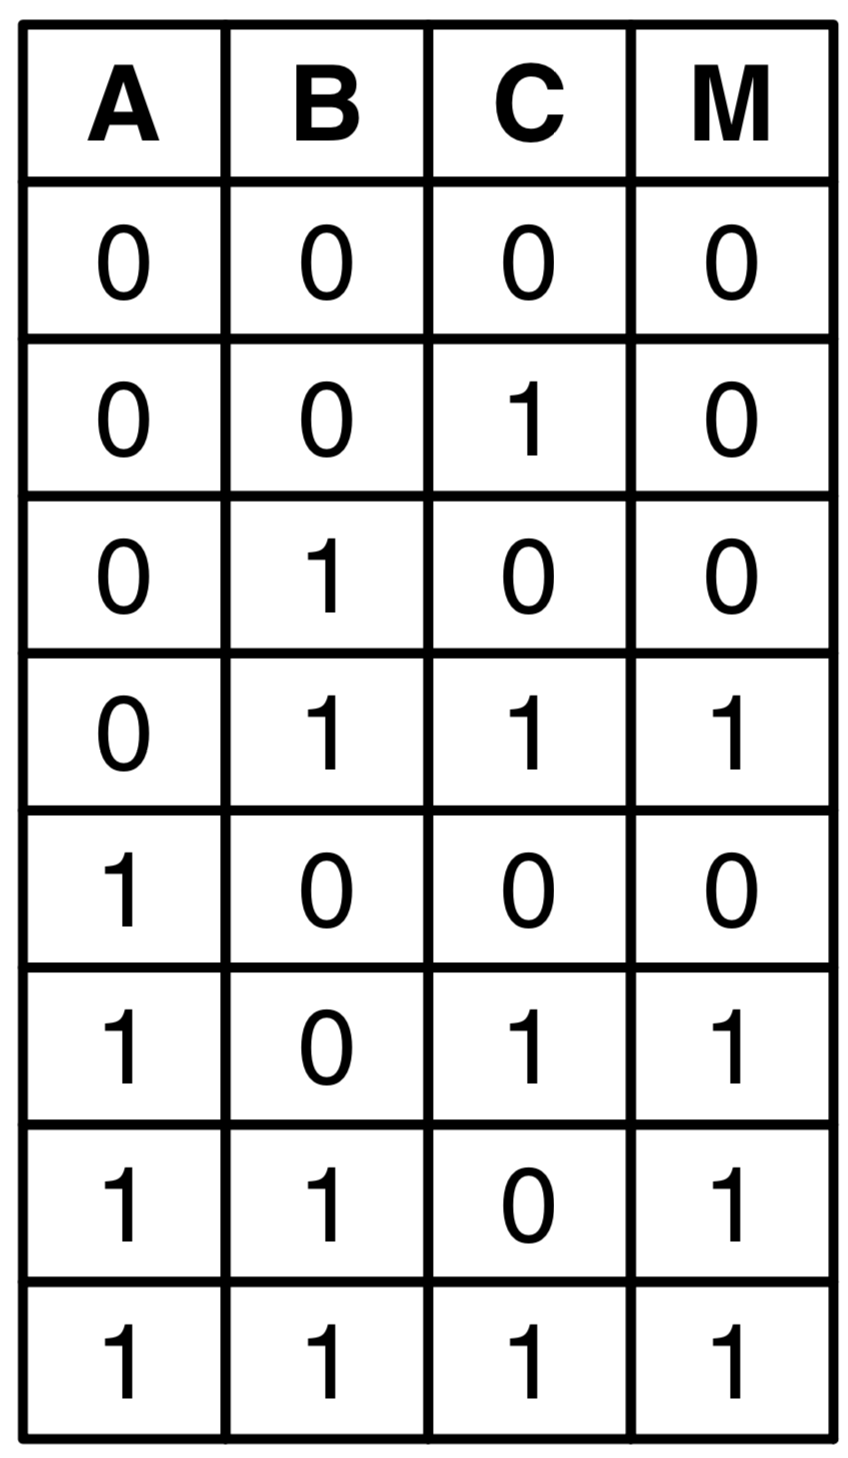
\includegraphics[width=0.4\linewidth]{images/processeur_porte_table.png}
            \caption{Table de vérité d'un circuit souhaité
            \label{pic:processeur_porte_table}}
        \end{subfigure}
        ~ %add desired spacing between images, e. g. ~, \quad, \qquad, \hfill etc.
          %(or a blank line to force the subfigure onto a new line)
        \begin{subfigure}[b]{0.40\linewidth}\centering
            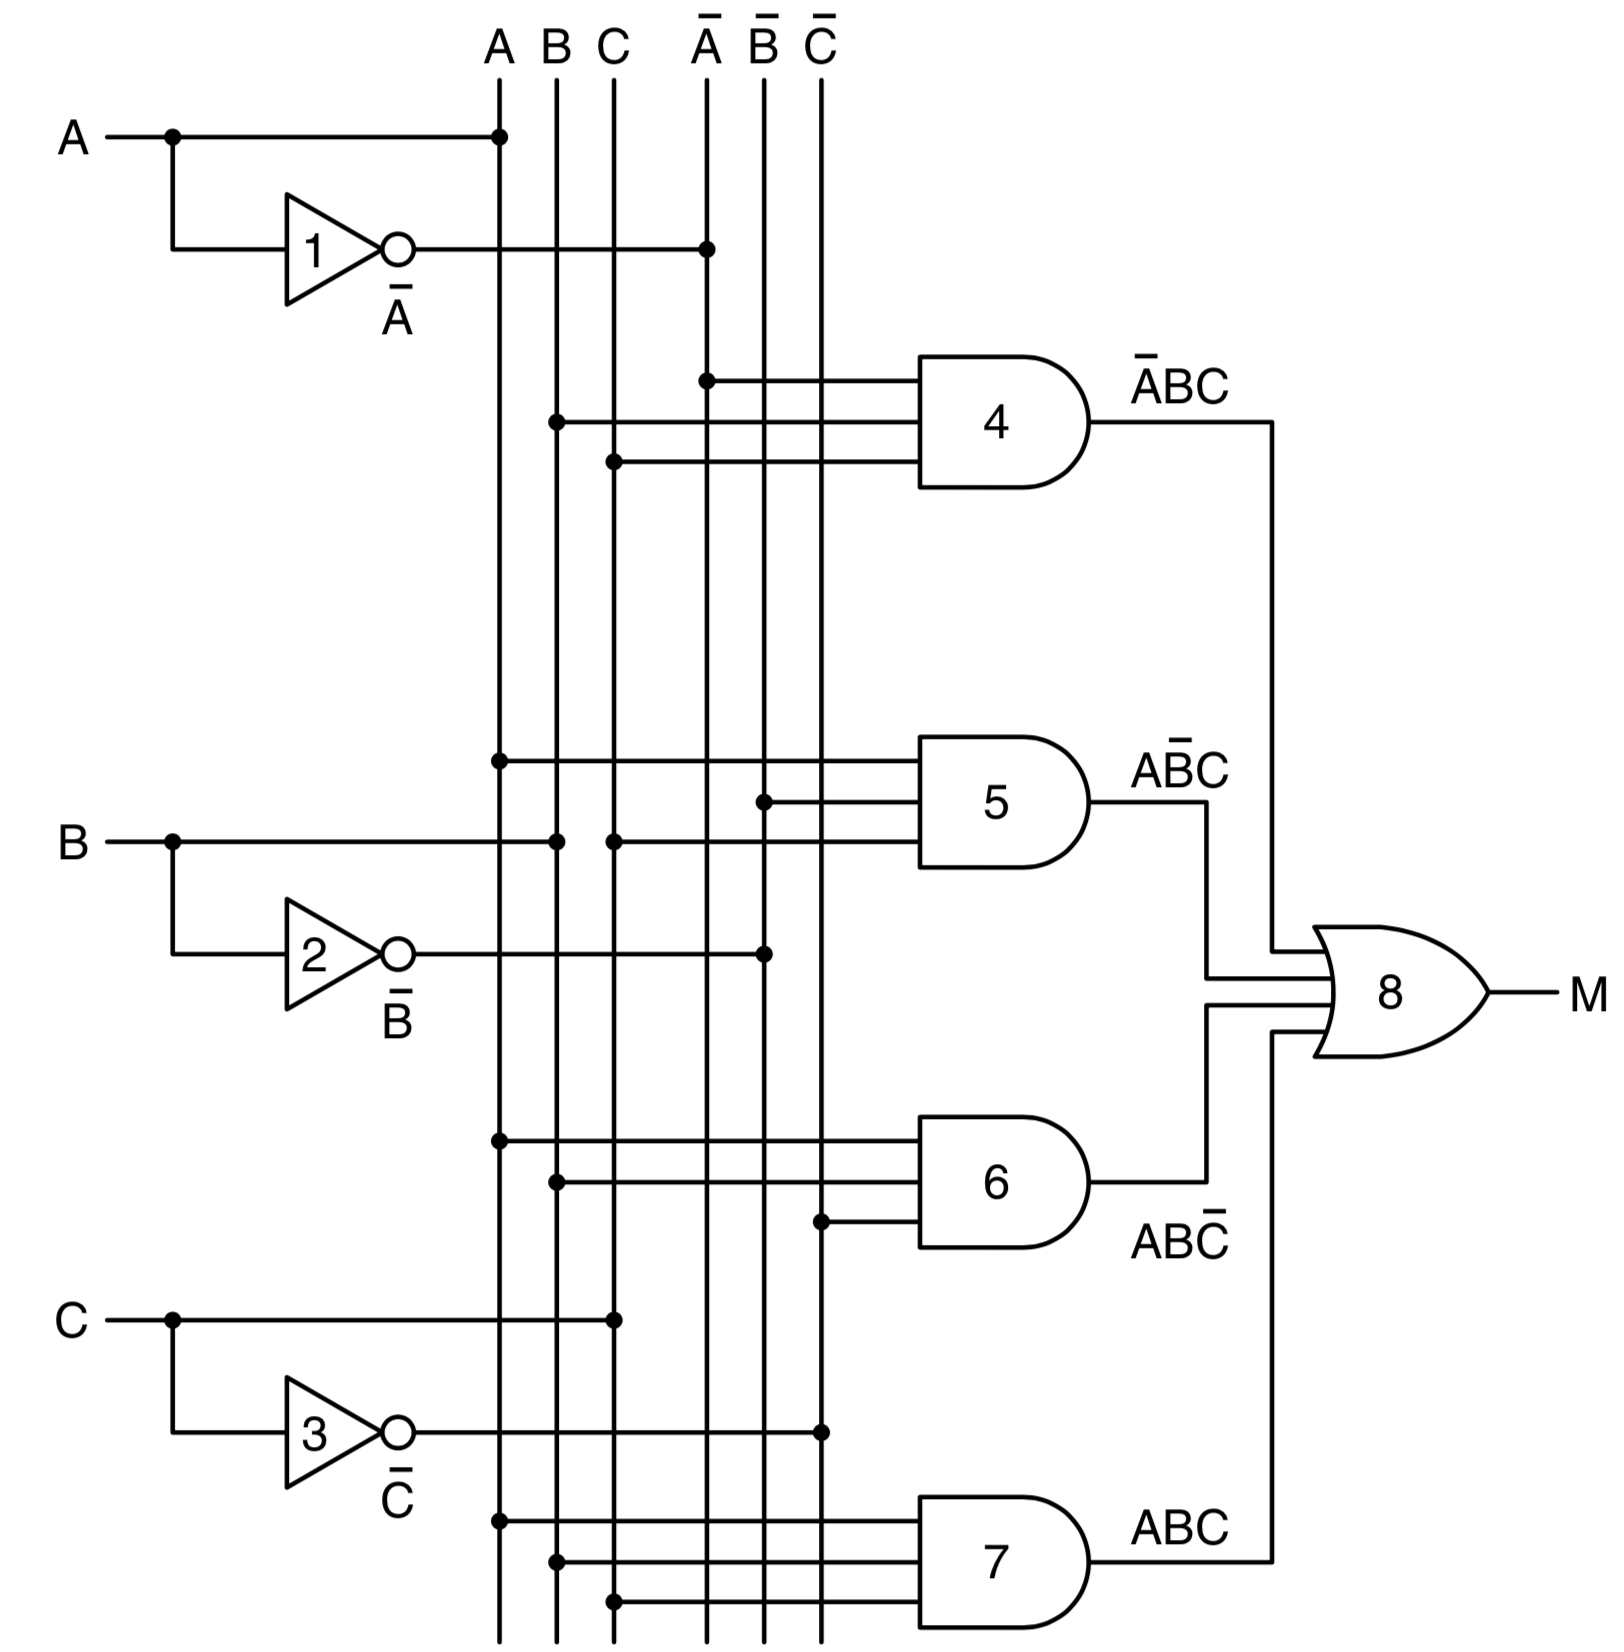
\includegraphics[width=\linewidth]{images/processeur_porte_schema.png}
            \caption{Circuit logiques  utilisant 8 portes
            \label{pic:processeur_porte_schema}}
        \end{subfigure}
        \caption{A partir d'une table de vérité, on peut générer le circuit logique correspondant \cite{tanenbaum2016structured}  \label{pic:processeur_porte_schema_2}}
    \end{figure}
    
    


\subsection{Circuits logiques}
%%%%%%%%%%%%%%%%%%%%%%%%%%%%%%%%%%%%%%%%%%%%%%%%%%%%%%%%%%%%%%%%%%%

    À partir des portes logiques et de leur analyse avec l'algèbre de Boole des circuits plus complexes peuvent être élaborés qui peuvent être regroupés en deux grandes familles: les circuits logiques de base  et les circuits logiques à mémoire. La principale différence entre les deux vient de leur capacité à retenir une information. 

    \subsubsection{Les circuits logiques de base}
    
        Les circuits logiques de base contiennent les circuits intégrés qui sont des circuits pouvant comporter quelques centaines de portes (circuit SSI, MSI) ou plusieurs centaines de milliers (circuit LSI et VLSI) \cite{barbe2013very}.
    
        Les circuits combinatoires ne possédant pas de mémoire interne pouvant influer sur le résultat ne dépendent que des entrées. Parmi eux, nous pouvons citer le multiplexeur (qui permets de choisir une entrée parmi plusieurs), les circuits arithmétiques (additionneur, décaleur) et l’horloge. 
        
        Ces circuits de bases sont utilisés pour construire les unités arithmétiques et logiques des processeurs ou des \gls{FPU} présentées dans la \autoref{sec:fpu}.
    
    
    \subsubsection{Les circuits à mémoire}
    
        La deuxième famille de circuits comporte un des composants fondamentaux des ordinateurs qui permet la construction de mémoires (\autoref{fig_processeurs_porte_bascule}). Cette capacité de mémorisation est permise grâce à l'utilisation de deux portes \verb|NON-ET| (\autoref{pic_processeurs_porte_bascule_nand}) ou \verb|NON-OU| (\autoref{pic_processeurs_porte_bascule_nor}). La particularité de ce circuit, appelé bascule, est la réutilisation de la sortie d'une porte comme entrée d'une seconde, lui permettant le stockage d'une valeur. 
        Les deux entrées d'un tel circuit peuvent être assimilées à une commande de mise à 1 (\textit{set}) et de remise à 0 (\textit{reset}).
        
        \begin{figure}
            %\centering
            \begin{subfigure}[]{0.48\linewidth}\centering
                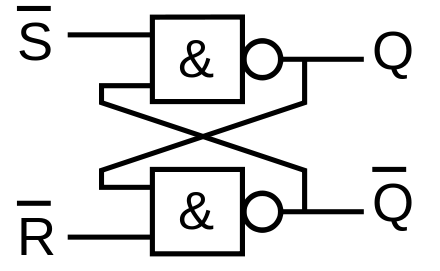
\includegraphics[width=0.60\linewidth]{images/processeurs_porte_bascule_nand.png}
                \caption{Implémentation à partir de portes \textit{NON-ET}}
                \label{pic_processeurs_porte_bascule_nand}
            \end{subfigure}
            ~ %add desired spacing between images, e. g. ~, \quad, \qquad, \hfill etc. 
              %(or a blank line to force the subfigure onto a new line)
            \begin{subfigure}[]{0.48\linewidth}\centering
                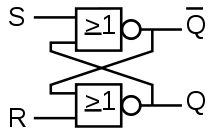
\includegraphics[width=0.60\linewidth]{images/processeurs_porte_bascule_nor.png}
                \caption{Implémentation à partir de portes \textit{NON-OU}}
                \label{pic_processeurs_porte_bascule_nor}
            \end{subfigure}
            \caption{Réalisation d'une bascule à partir de deux types de portes. La bascule maintient son état actuelle tant que les signaux d'entrée ne changent pas}
            \label{fig_processeurs_porte_bascule}
        \end{figure}


\subsection{Les mémoires RAM} \label{sec:ram}
%%%%%%%%%%%%%%%%%%%%%%%%%%%%%%%%%%%%%%%%%%%%%%%%%%%%%%%%%%%%%%%%%%%

    La mémoire à accès aléatoires ou \textit{Random Acces Memory} (RAM) est une mémoire dont le temps d'accès ne dépend pas de la position de l'information contrairement aux disques ou aux bandes magnétiques. Sur ces deux support le temps d'accès pouvait varier en fonction de l'emplacement actuel de la tête de lecture et de la prochaine donnée à lire. La RAM est une mémoire volatile, l'information stockée n'est pas persistante lorsque la mémoire n'est plus alimentée. Il y a eu beaucoup d'évolution des différentes technologies RAM depuis leur création. Il en existe différents types, ayant leurs avantages et leurs inconvénients. Dans une plateforme actuelle, deux types de mémoires RAM sont principalement utilisées: la RAM statique (SRAM, \autoref{pic_processeurs_porte_sram}) et la RAM dynamique (DRAM, \autoref{pic_processeurs_porte_dram}). La raison principale de la présence de deux types de RAM vient de leur différence de coût de production. La SRAM, bien que plus rapide, est aussi beaucoup plus chère. Cette différence de prix s'explique par l'architecture des deux mémoires (\autoref{fig_processeurs_ram}).
    
    
    \begin{figure}
        %\centering
        \begin{subfigure}[]{0.48\linewidth}\centering
            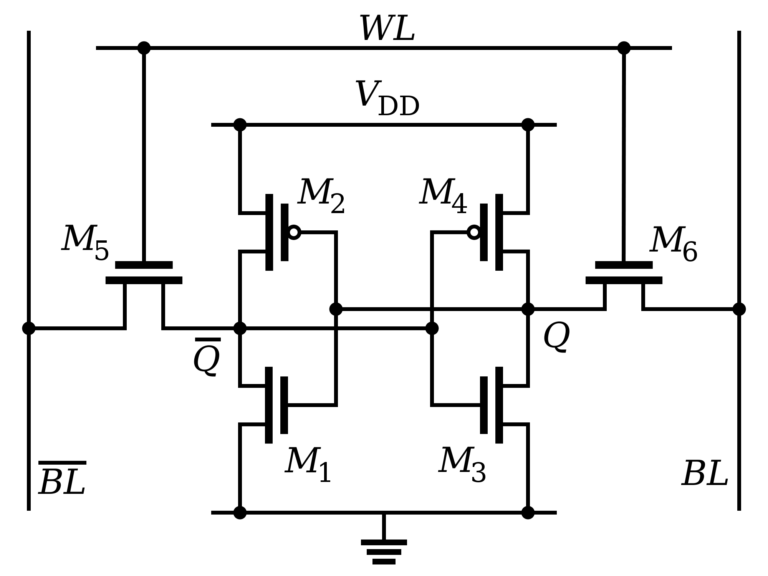
\includegraphics[width=0.80\linewidth]{images/processeurs_porte_sram.png}
            \caption{Mémoire vive statique (SRAM) utilisant 6 transistors}
            \label{pic_processeurs_porte_sram}
        \end{subfigure}
        ~ %add desired spacing between images, e. g. ~, \quad, \qquad, \hfill etc. 
          %(or a blank line to force the subfigure onto a new line)
        \begin{subfigure}[]{0.48\linewidth}\centering
            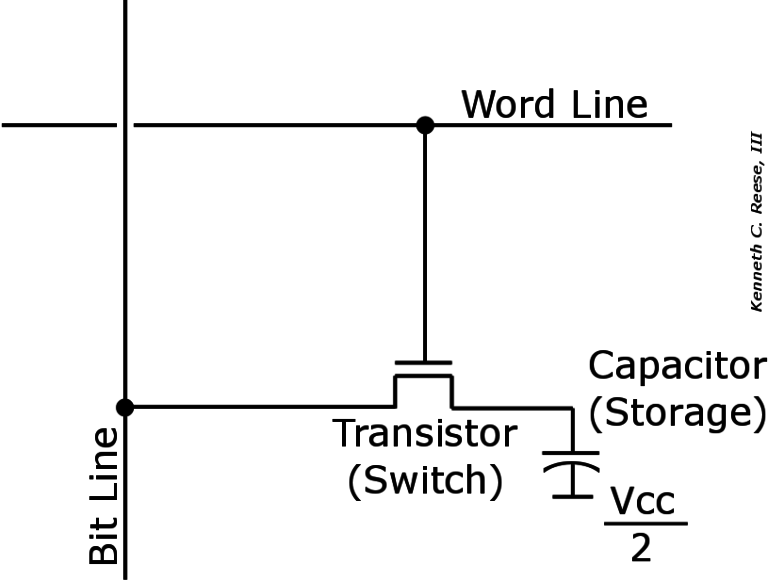
\includegraphics[width=0.80\linewidth]{images/processeurs_porte_dram.png}
            \caption{Mémoire vive dynamique (DRAM) utilisant un condensateur et un transistor}
            \label{pic_processeurs_porte_dram}
        \end{subfigure}
        \caption{Deux types de RAM très utilisées dans les architectures. La différence de complexité de leur circuit électronique explique la différence de prix entre les deux technologies}
        \label{fig_processeurs_ram}
    \end{figure}
    
    \subsubsection{La SRAM} 
    
        La RAM statique est un circuit logique qui utilise 6 transistors (voir \autoref{pic_processeurs_porte_sram}) pour représenter les états 0 et 1 (bien qu'il existe des variantes utilisant 4, 8 ou même 10 transistors). Une SRAM à 6 transistors en utilise 4 pour stocker l'information. Deux transistors additionnels sont utilisés pour contrôler leur accès durant leur lecture ou écriture.
        Il est courant d'utiliser différents types de SRAM dans les différents niveaux de caches pour optimiser la densité (mémoire de plus grande capacité) ou la vitesse d'accès (latence réduite). Par exemple, le premier niveau de cache est généralement optimisé pour la vitesse d'accès, contrairement aux caches de niveau supérieur de plus grande capacité.
    
    
    \subsubsection{La DRAM} 
    
        La RAM dynamique a une structure plus simple que la SRAM qui n'est composée que d'un transistor et d'un condensateur (voir \autoref{pic_processeurs_porte_dram}). La valeur du bit est déterminée par la charge (positive ou négative) du condensateur. Ainsi, que la valeur stockée dans le condensateur soit \verb|VRAI| ou \verb|FAUX|, le condensateur doit être chargé. Cependant, la lecture d’une cellule décharge le condensateur, il faut donc, même lors d’une lecture, le recharger. De plus, à cause des fuites de courant (\textit{power leakage}) les condensateurs doivent être rafraîchis en permanence. La fréquence de rafraîchissement est de l'ordre de 1\% à 5\% du temps total d'utilisation de la mémoire. Ces deux contraintes font de la DRAM une mémoire très consommatrice en énergie. Grâce à leur faible nombre de transistors, la densité des mémoires DRAM est élevée, permettant la construction de mémoire de grande capacité (en GB). Ainsi, la quasi-totalité des ordinateurs des 50 dernières années ont une mémoire centrale utilisant de la DRAM. 
        La charge et la décharge du condensateur n’étant pas instantanés, la DRAM est beaucoup plus lente que la SRAM (une cellule ne pouvant pas être accédée pendant son rafraîchissement). 
    
    %Il existe plusieurs types de DRAM: DDR, GDDR, QDR, HBMC, HMC.
    
    
    \subsubsection{SRAM vs DRAM}
    
        L'avantage de la SRAM est sa rapidité de fonctionnement et sa faible consommation électrique. Contrairement à la DRAM, la SRAM est statique, elle conserve l'information et ne nécessite pas de rafraîchissement périodique pour conserver la donnée enregistrée. Cependant, elle s'efface si aucune tension ne lui est appliquée en continu.
        Le principal inconvénient de la SRAM vient de son coût de fabrication ainsi que leur faible densité (due à l'utilisation de 6 transistors)
    
    
        % Please add the following required packages to your document preamble:
        % \usepackage{graphicx}
        \begin{table}[]
        \centering
        %\resizebox{\textwidth}{!}{%
        \begin{tabular}{l|c|c|}
        \cline{2-3}
         & SRAM & DRAM \\ \hline
        \multicolumn{1}{|l|}{Prix/bit} & élevé & bas \\ \hline
        \multicolumn{1}{|l|}{Vitesse d'accès} & rapide & lent \\ \hline
        \multicolumn{1}{|l|}{Latence} & 0.5-5 ns & 50-70 ns \\ \hline
        \multicolumn{1}{|l|}{Rafraichissement} & non & oui \\ \hline
        \multicolumn{1}{|l|}{Consommation} & basse & élevée \\ \hline
        \multicolumn{1}{|l|}{Énergie/bit} & 0,1 pj & 1 pj \\ \hline
        \multicolumn{1}{|l|}{Densité} & faible (6 transistors par bit) & élevée (1 transistor par bit) \\ \hline
        \multicolumn{1}{|l|}{Complexité} & grande & faible \\ \hline
        \multicolumn{1}{|l|}{Utilisation} & Cache & Mémoire centrale \\ \hline
        \end{tabular}%
        %}
        \caption{Comparaison des caractéristiques principales des mémoires SRAM et DRAM.}
        \label{tab:my-table}
        \end{table}
            
    


\subsection{Évolution des transistors}
%%%%%%%%%%%%%%%%%%%%%%%%%%%%%%%%%%%%%%%%%%%%%%%%%%%%%%%%%%%%%%%%%%%

    
    La vitesse de calcul d'un processeur ou la capacité de stockage d'une mémoire sont directement liées au nombre de transistors disponibles sur une puce. 
    Plus un processeur aura de transistors, au plus il pourra calculer rapidement (ajout de coeur, meilleures unités de calculs). Plus une mémoire aura de transistors, au plus elle pourra contenir de cellule RAM et donc avoir une grande capacité de stockage. La performance des systèmes informatiques est donc directement liée aux technologies de transistors utilisées. 
    
    
    \subsubsection{Évolution du nombre de transistors.} \label{sec:moore}
    
        L'évolution du nombre de transistors sur une puce a été prédite par l'un des trois fondateurs de la société Intel, Gordon Moore. En 1965, Gordon Moore prévoit que le nombre de transistors d'un puce doublera chaque année, sur une même surface et pour un coût constant \cite{Moore1998}. Il réévaluera cette période à 2 ans en 1975 \cite{Moore75}, ce qui correspond parfaitement avec l'évolution réelle jusqu'à ces dernières années (\autoref{pic_Moore_prediction}). Les mémoires RAM étant constituées de transistors, leur évolution a aussi été guidée par la loi de Moore (\autoref{processeurs_porte_moore_dram}).
        
        
        
        
        \begin{figure}
            %\centering
            \begin{subfigure}[]{0.48\linewidth}\centering
                \vspace{1cm}
                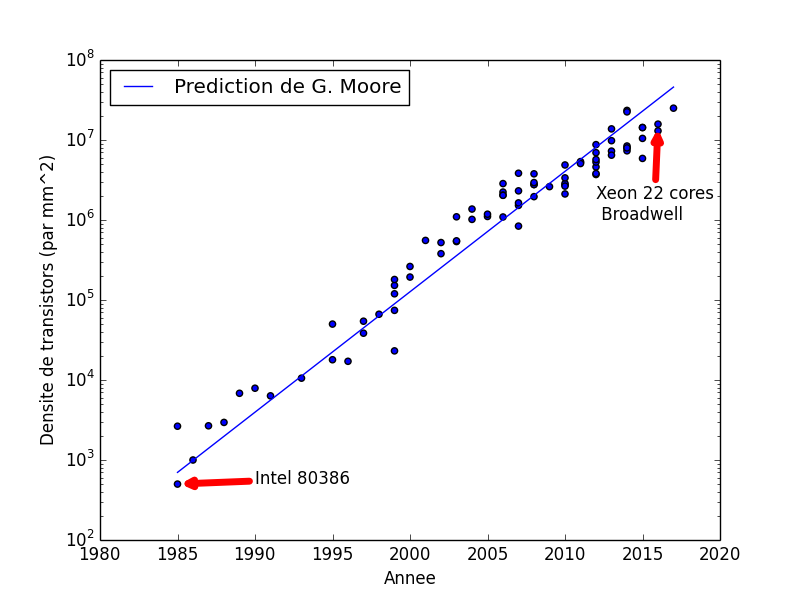
\includegraphics[width=\linewidth]{images/Chapitre1/Moore_prediction.png}
                \caption{\label{pic_Moore_prediction} Évolution du nombre de transistors des processeurs Intel (données \cite{Wikipedia2019Transistor})}
            \end{subfigure}
            ~ %add desired spacing between images, e. g. ~, \quad, \qquad, \hfill etc. 
              %(or a blank line to force the subfigure onto a new line)
            \begin{subfigure}[]{0.48\linewidth}\centering
                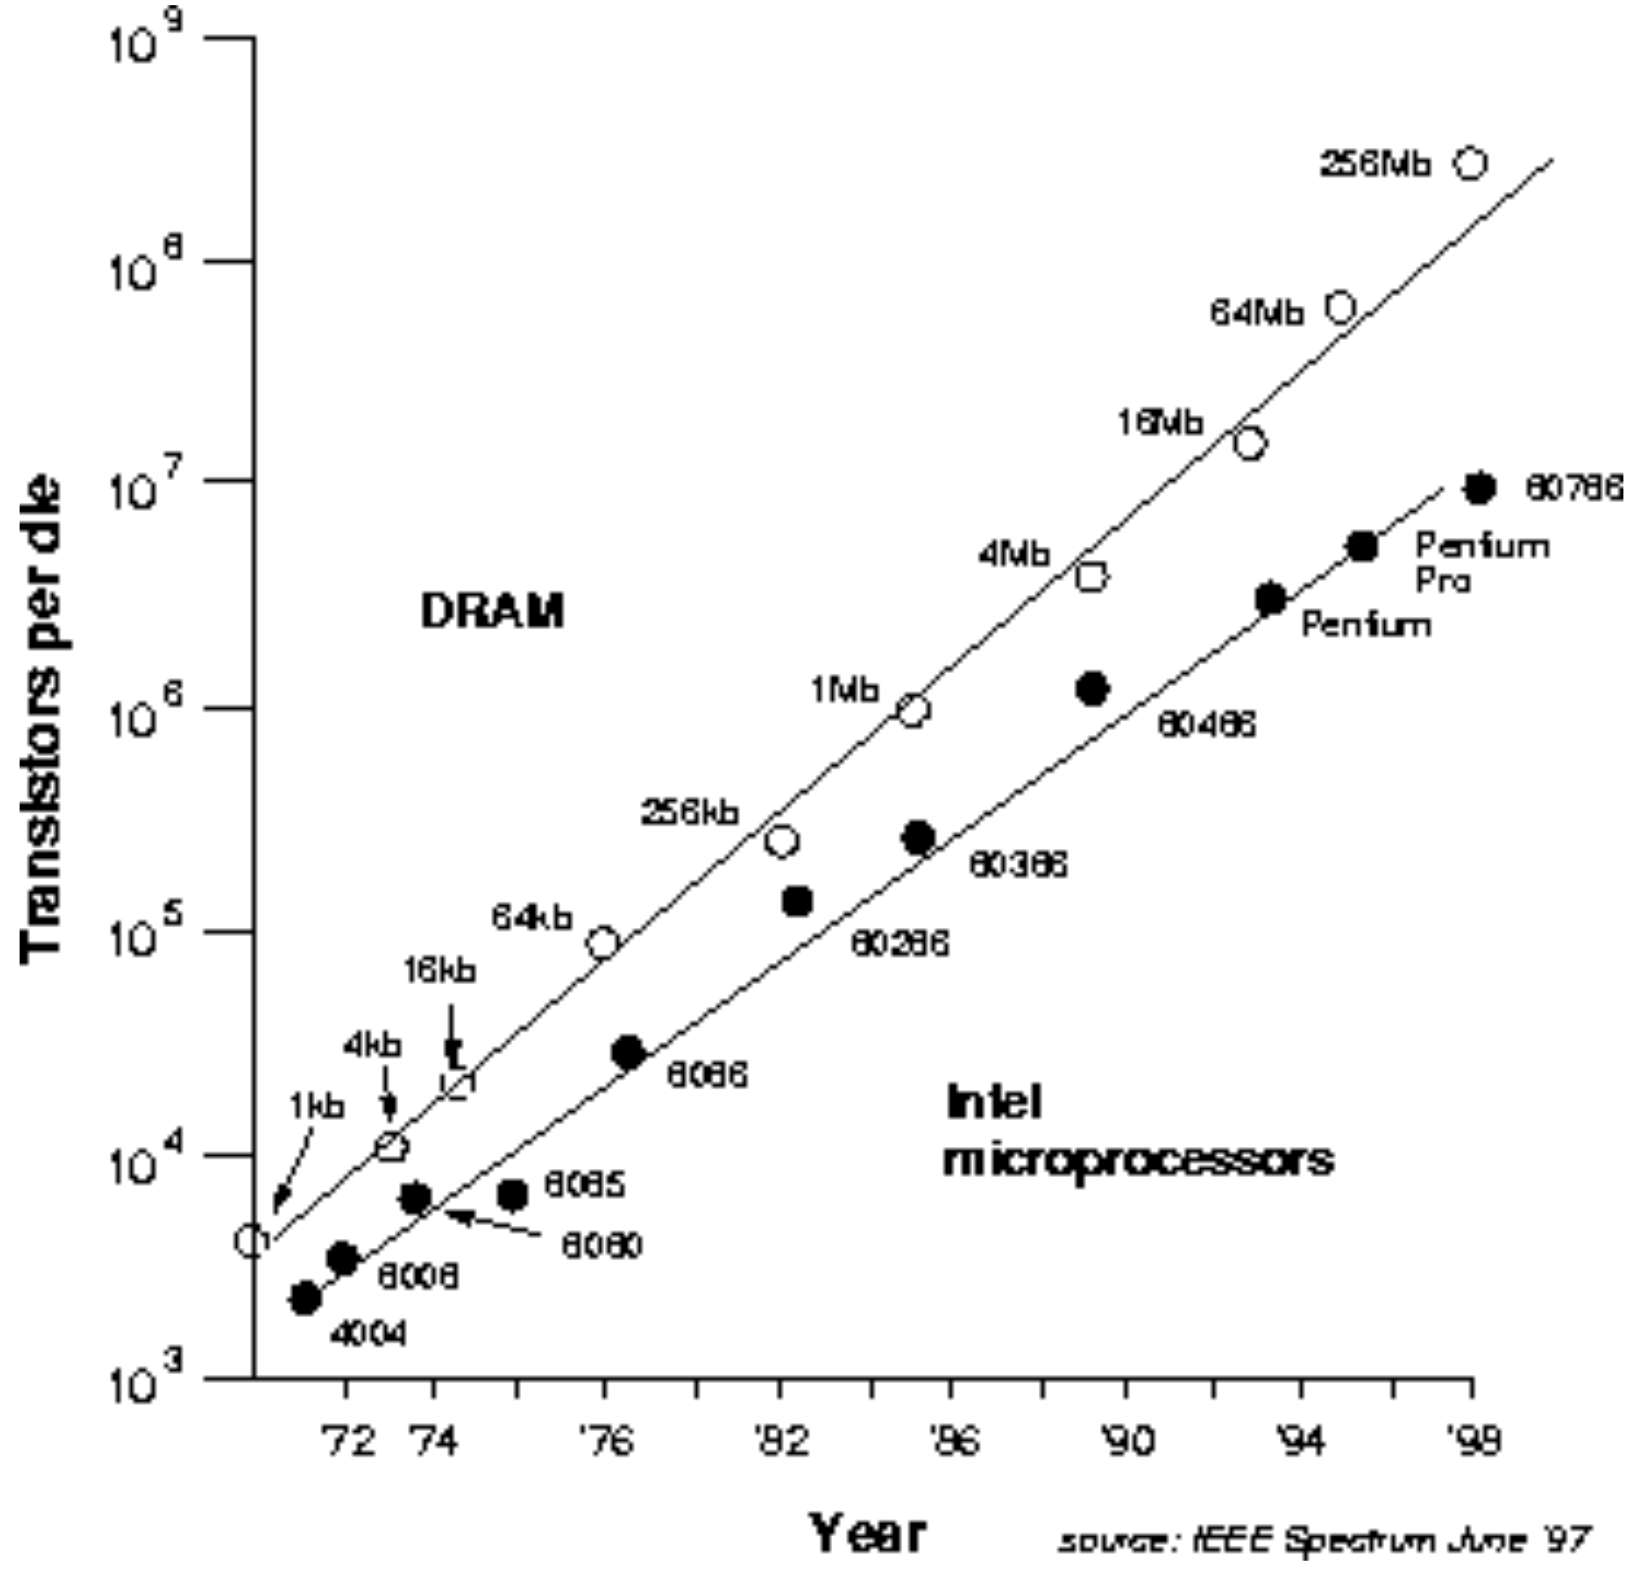
\includegraphics[width=0.9\linewidth]{images/processeurs_porte_moore_dram.png}
                \caption{La loi de Moore s'applique aux processeurs comme aux mémoires DRAM.}
                \label{processeurs_porte_moore_dram}
            \end{subfigure}
            \caption{La loi de Moore décrit l'évolution de la densité de transistors qui double tous les deux ans pour un prix constant.}
            \label{fig_processeurs_moore}
        \end{figure}
        
        
    
    
    
    \subsubsection{Coût de la gravure.}
    
        Depuis plus de cinquante ans, les fondeurs (les industriels responsables de la gravure des processeurs) tels que Samsung Electronics, TSMC, Intel et GlobalFoundries ont développé de nombreuses techniques et technologies pour réduire la taille des transistors (voir \autoref{processeurs_porte_fondeurs}). Aujourd'hui, de nombreuses étapes sont nécessaires pour transformer une plaque de silicium (la plus pure possible) en processeurs: dopage, déposition d'une couche de résine, gravure, traitement thermique, revêtement par couche mince, découpe, encapsulation... \cite{AnthonyNelzinSantos2018}.
        
        Les procédés de fabrication étant plus complexes, les usines de fabrication coûtent elles aussi de plus en plus cher. L'augmentation du coût des fonderies a elle aussi été prédite par la seconde loi de Gordon Moore (ou \textit{loi de Rock}), qui estime que leur prix double tous les 4 ans \cite{schaller1997moore}. 
        
        Bien que les coûts de fabrication augmentent, la taille de gravure s’affine et permet de mettre plus de transistors sur une même surface, permettant ainsi à l’industrie de suivre la cadence dictée par la loi de Moore (\autoref{pic_Moore_explique}). Cependant, les finesses de gravures utilisées aujourd'hui sont tellement faibles qu'elles atteignent une limite physique, celle de la taille des atomes. À des tailles proches de quelques atomes, les courants électriques ne sont plus stables et la course à la réduction des finesses de gravure n'a jamais été aussi difficile. Voilà plusieurs années, qu'Intel ne parvient plus à descendre sous les 10 nm. Les procédés à mettre en oeuvre pour y parvenir sont si complexes, qu'il est courant de parler de la fin de la loi de Moore \cite{theis2017end}. En 2019, Samsung annonce qu'il a mis au point une technologie permettant la gravure des premiers processeurs en 3 nm dès 2021 \cite{AdrianBRANCO2019}. 
        
        
        \begin{figure}[htbp]
            \centering
            \begin{subfigure}[b]{0.40\linewidth}\centering
                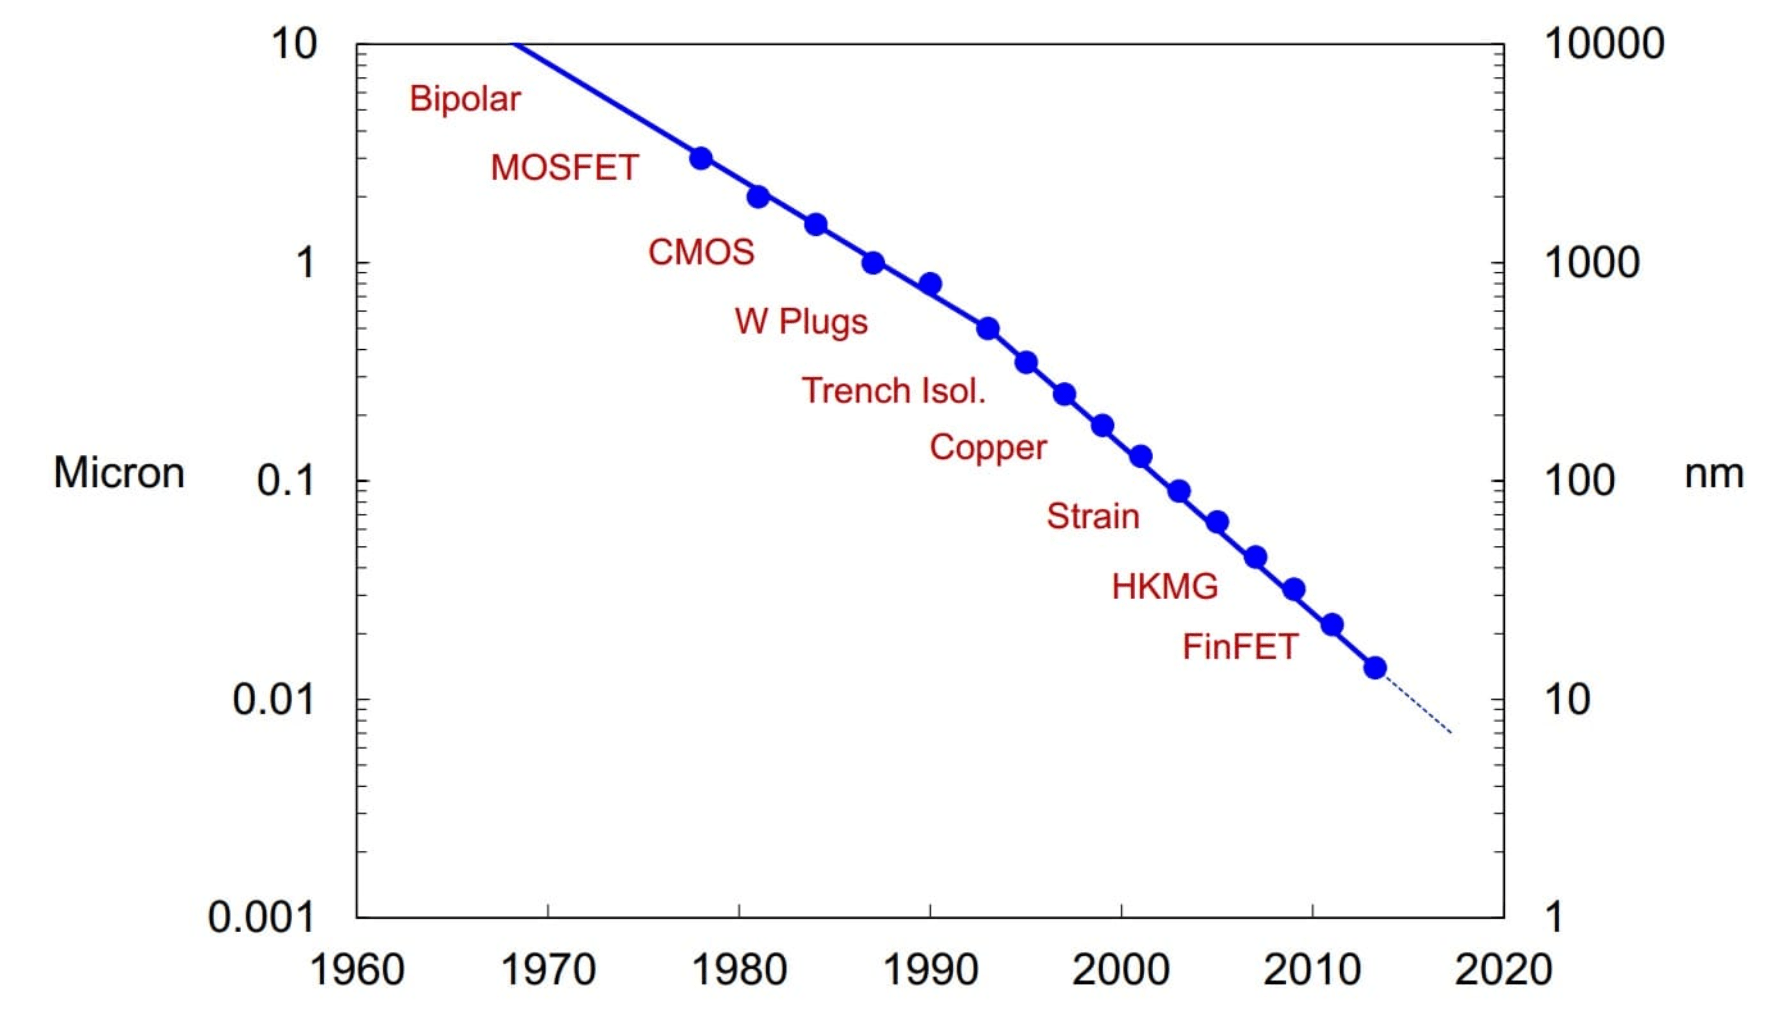
\includegraphics[width=\linewidth]{images/processeurs_porte_fondeurs.png}
                \caption{\label{processeurs_porte_fondeurs} Les technologies utilisées pour la gravure ont évoluées, rendant les fonderies plus performantes mais aussi plus chères (source Intel).}.
            \end{subfigure}
            ~ %add desired spacing between images, e. g. ~, \quad, \qquad, \hfill etc.
              %(or a blank line to force the subfigure onto a new line)
            \begin{subfigure}[b]{0.50\linewidth}\centering
                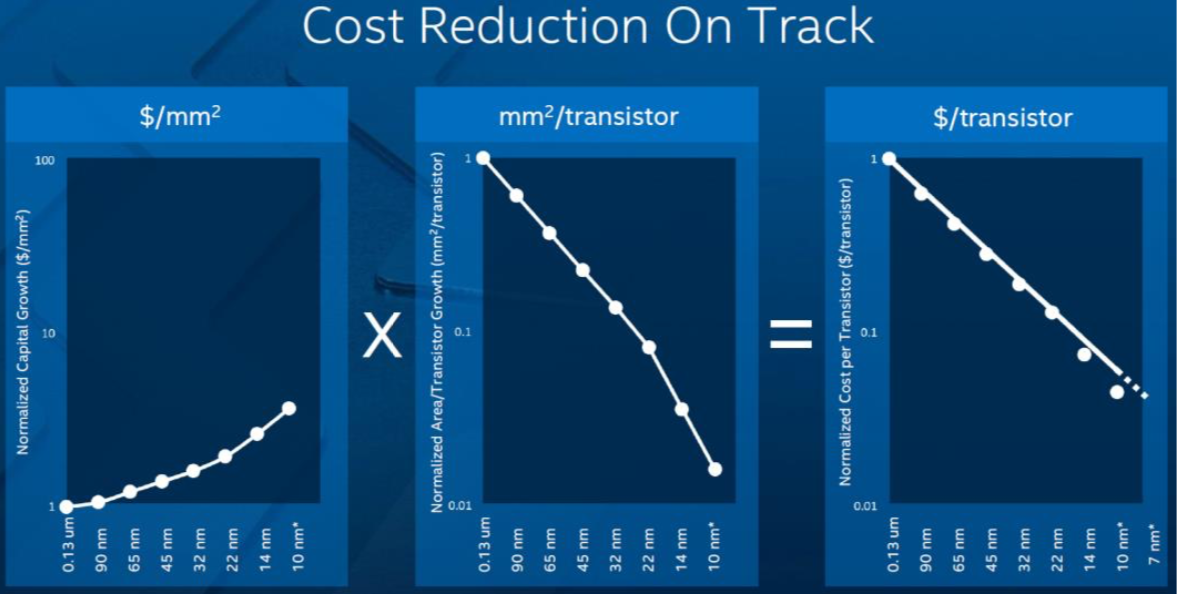
\includegraphics[width=\linewidth]{images/processeurs_porte_moore.png}
                \caption{\label{pic_Moore_explique} Bien que le prix des fonderie augmente, le nombre de transistors gravable sur une puce augmente plus rapidement. Conséquence de la loi de Moore: le prix par transistor diminue exponentiellement.}
            \end{subfigure}
            \caption{Les nouvelles technologies utilisées dans les fonderies permettent de graver des transistors toujours plus petits.}\label{pic_fonderie}
        \end{figure}
 
        \section{L'architecture} \label{sec:micro}
%%%%%%%%%%%%%%%%%%%%%%%%%%%%%%%%%%%%%%%%%%%%%%%%%%%%%%%%%%%%%%%%%%%
%%%%%%%%%%%%%%%%%%%%%%%%%%%%%%%%%%%%%%%%%%%%%%%%%%%%%%%%%%%%%%%%%%%

Dans la section précédente nous avons présenté les transistors, les éléments de bases des ordinateurs. Ces transistors sont groupés en portes logiques pour construire des circuits électroniques. Cette section présente comment ces circuits sont utilisés pour construire la microarchitecture d'un ordinateur capable d'exécuter les instructions. L'objectif n'est pas de présenter la totalité de l'architecture, mais seulement les éléments importants nécessaires à notre travail de thèse. Nous commençons dans la \autoref{sec:archi_origine} par définir une architecture et présenter les principaux modèles utilisés aujourd'hui. Dans les sections suivantes, nous nous intéressons aux évolution technologiques des processeurs qui ont permis d'améliorer l'efficacité d'exécution des instructions (\autoref{sec:efficacite}), d'accélérer leur exécution (\autoref{sec:accelerer}) et enfin de rendre leur exécution en parallèle possible (\autoref{sec:para}).



\subsection{Architecture de processeur: origine et évolutions majeures} \label{sec:archi_origine}

    
Afin d'éviter toutes confusions, nous rappelons la définition de la microarchitecture et de l'ISA car ces termes sont souvent confondus dans la littérature:

\begin{itemize}
    \item  \textbf{La couche ISA} (\textit{Instruction Set Architecture}) regroupe les instructions, leur mode (système ou utilisateur), les registres utilisables, l'organisation du système mémoire (alignement, espace d'adressage) ... 
    C'est une spécification formelle établie, qui peut être utilisée par plusieurs fabricants de microarchitectures \cite{tanenbaum2016structured}. Intel publie fréquemment la documentation de l'ISA x86 \cite{Intel2018}. Elle forme l'interface entre le matériel et le logiciel et permet la compatibilité de programme sur des microarchitectures de différents constructeurs. 
    Grâce à la couche ISA, différents langages de programmation peuvent être utilisés pour écrire les applications. Le compilateur s'occupe alors de les traduire dans un langage de bas niveau pouvant utiliser l'ISA (langage assembleur). Ce langage est tellement proche de la couche ISA que les deux termes sont souvent mélangés. Les ISA existantes sont listées dans la \autoref{sec:isa}. 

    \item \textbf{La microarchitecture} correspond à l'implémentation matérielle de l'ISA. Ce sont deux couches distinctes, la seconde n'ayant pas forcément besoin d'avoir connaissance de la première (bien que pour des raisons de performances cela soit préférable). En ayant connaissance de la microarchitecture, le compilateur pourra réordonner ou modifier des instructions pour tirer parti du pipeline ou d'un processeur vectoriel. La conception d'une nouvelle microarchitecture doit commencer par choisir l'ISA à implémenter (si possible existante pour permettre la compatibilité des programmes). Les différences principales entre deux microarchitectures implémentant la même ISA sont leur différence de performances et de coût. Les processeurs Intel et AMD implémentent la même ISA \verb|x86|. La performance et le nombre d'instructions supportés par les deux architectures sont cependant différents.
    
    \item Il arrive que le terme d'\textbf{architecture} soit employé à la place du terme ISA, par exemple par IBM en 1964 \cite{amdahl1964architecture}.  Aujourd'hui, ce terme est souvent utilisé pour faire référence à la fois à l'ISA et à la \textit{microarchitecture}. Il est courant d'entendre parler d'\textit{architecture x86} pour faire référence à une microarchitecture implémentant l'ISA \verb|x86|.\\ 
\end{itemize}

    
    \subsubsection{Les premiers processeurs}

        L'origine des premiers calculateurs remonte bien avant l'invention des systèmes électroniques. Les premières machines à calculer sont apparues à la fin du 16e siècle, conçues par Blaise Pascal et Gottfried Wilhelm Leibnitz \cite{Vie1996}. Les opérations en base 10 étaient à réaliser par l'utilisateur au moyen de roues dentées. 
        Pour automatiser le recensement des 62 millions d'Américains vivant aux États Unis en 1890, le gouvernement lança un appel d'offres pour construire un système de traitement automatique. Herman Hollerith proposa alors d'utiliser un système de cartes perforées utilisé par des sociétés ferroviaires produit par la société Computing-Tabulating-Recording.  C'est en 1924 que la société fut renommée  International Business Machines (IBM). De 1937 à 1943, IBM construit pour l'Université de Harvard un calculateur géant capable de multiplier deux nombres de 23 chiffres en six secondes appelé  Automatic Sequence Controlled Calculator (ASCC) \cite{cortada2016computer}. Cet ordinateur fonctionnait à partir de dispositifs mécaniques et électromécaniques issus des machines à cartes perforées.
        
        Un autre projet de recherche à l'origine de l'ordinateur est celui mené par Allan Turing durant la Seconde Guerre mondiale. Utilisés pour décoder les messages chiffrés d'Enigma utilisée par l'armée allemande. Le câblage de ces premiers automates devait être refait lorsqu'on voulait appliquer un changement dans le traitement des opérations. On parlait alors de programmes extérieurs. Le calculateur d'Allan Turing avait une seule utilité, non des moindres, celle de déchiffrer des messages. Il ne pouvait cependant pas être utilisé pour réaliser d'autres calculs.
        

    \subsubsection{L'architecture Von Neumann}\label{sec:vonneumann}
        
        Bien que la microarchitecture des processeurs ait beaucoup évolué depuis leur création, l'organisation globale n'a pas changé. Aujourd'hui la majorité d'entre eux sont basés sur une architecture qui porte le nom  du scientifique à l'origine des premiers schémas : l'architecture \textit{Von Neumann}.

        C'est en 1945 que cette architecture a été présentée pour la première fois par John von Neumann dans un papier qu'il n'aura pas le temps de finir \textit{First Draft of a Report on the EDVAC}. Cependant, sur ce papier ne sont pas mentionnés les deux autres contributeurs que sont J. Presper Eckert et John Mauchly. Malheureusement pour eux, l'histoire ne retiendra que le nom du premier. Leur papier décrit les 3 premiers principes qui sont à l'origine des ordinateurs actuels. Le premier voulait que ces machines soient universelles, c'est-à-dire qu'elles puissent exécuter différents types de calculs. Le deuxième concernait leur programmation à l'aide d'instructions organisées dans des programmes qui, comme les résultats intermédiaires, peuvent être sauvés en mémoire. On parle alors de programmes enregistrés. Le troisième principe est l'implémentation de la rupture de séquence. Lors de l'exécution d'un programme, l'automate décide des instructions à exécuter, réalise des tests et des comparaisons pour faire des sauts dans le programme. La principale idée de cette architecture est la présence de trois modules principaux (voir \autoref{pic_cpu_von}):
         \begin{itemize}
            \item Une unité de traitement (CPU) qui contient une unité arithmétique et logique (ALU) qui s'occupe d'exécuter les opérations de bases (addition, multiplication, etc.) ainsi que de registres pour mémoriser les données utilisés pour leur exécution.
            \item L'unité de contrôle qui lit les instructions et organise leur exécution en s'occupant de demander les données nécessaires à la mémoire.
            \item Une mémoire qui contient toutes les données, mais aussi le code à exécuter contrairement aux anciennes architectures qui lisaient les programmes sur des cartes perforées, rubans, ou tableaux de connexion.
         \end{itemize}
          
        
        
        \begin{figure}
            \centering
            \begin{subfigure}[b]{0.45\linewidth}
                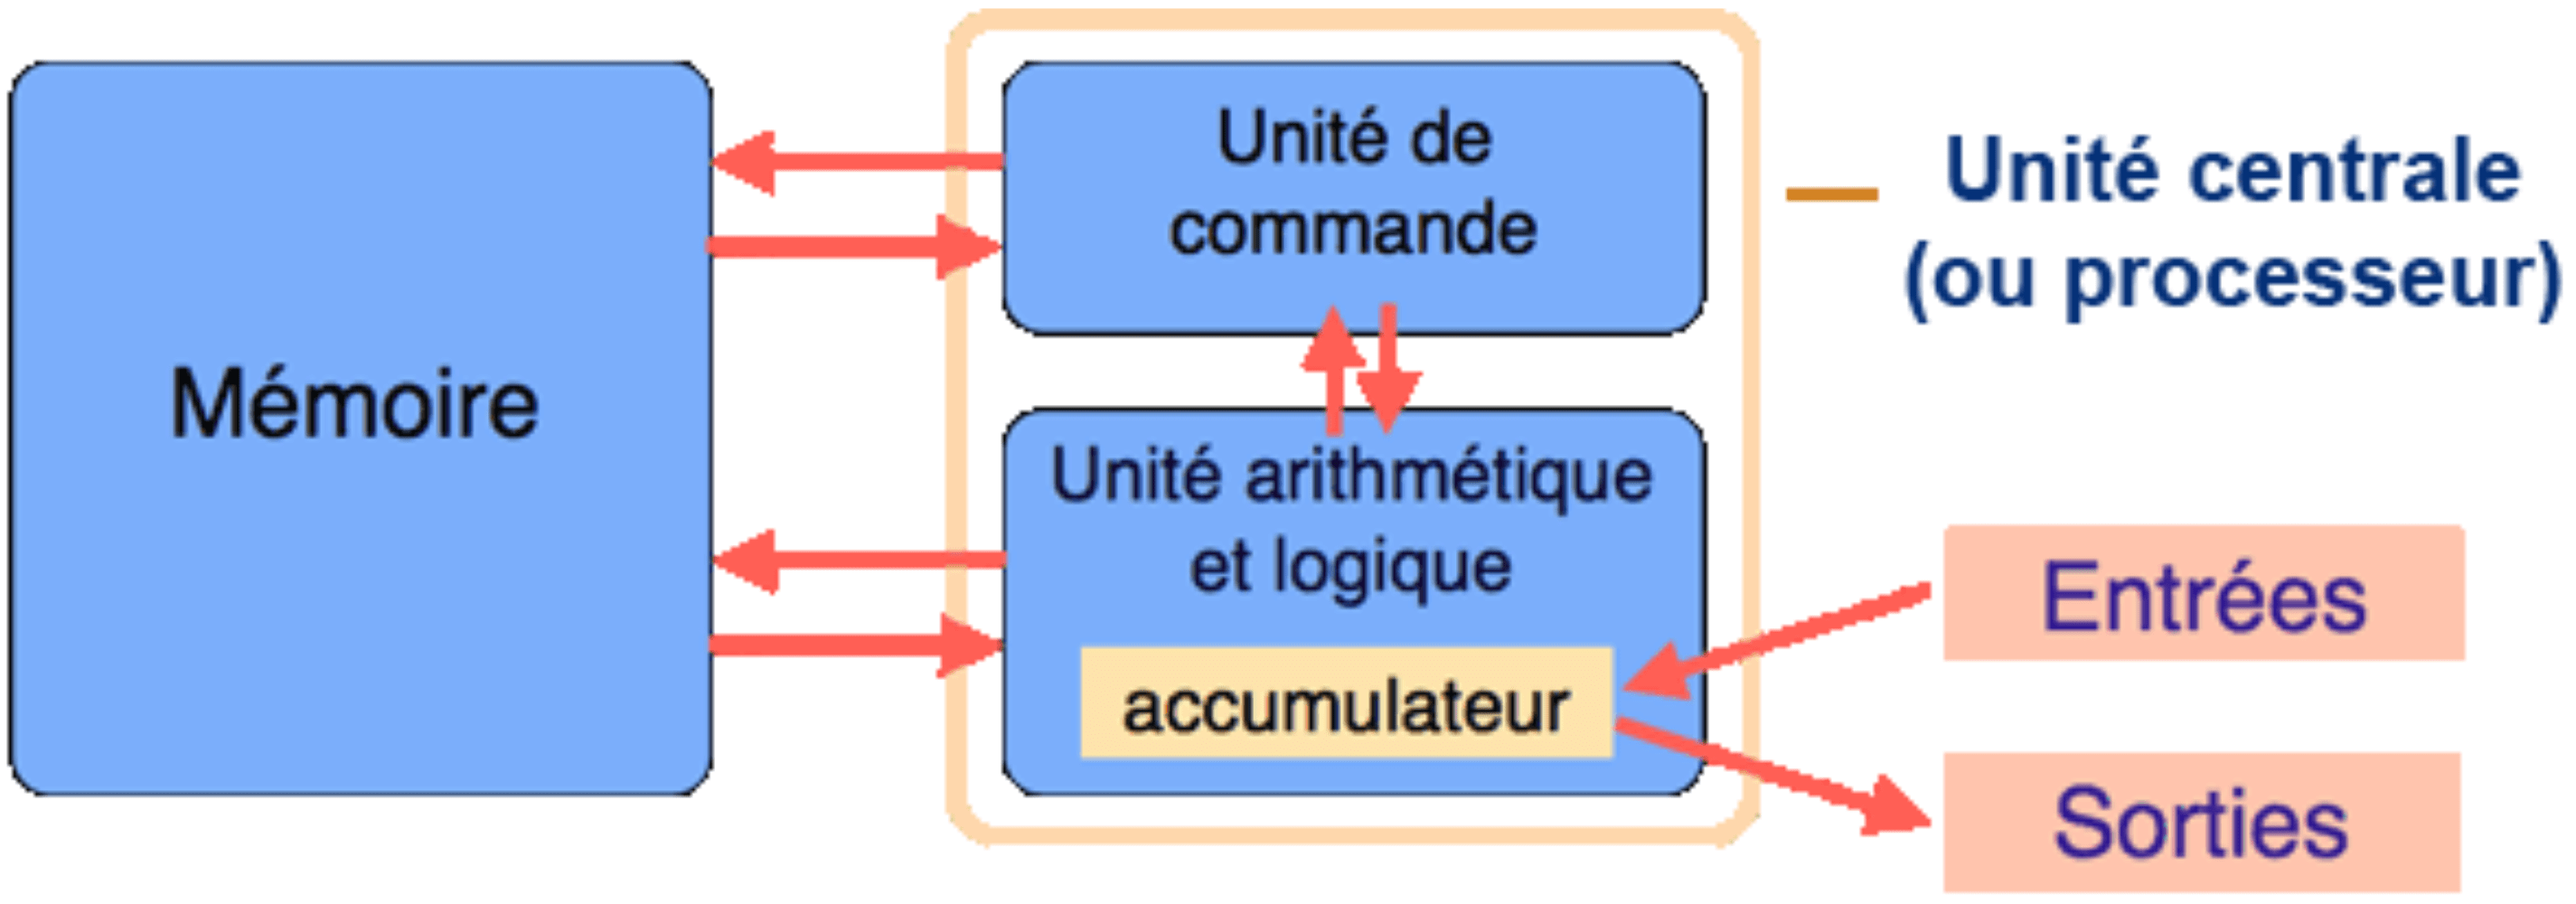
\includegraphics[width=\linewidth]{images/cpu_von1.png}
                \caption{Architecture Von Neuman initiale}
                \label{pic_cpu_von}
            \end{subfigure}
            ~ %add desired spacing between images, e. g. ~, \quad, \qquad, \hfill etc. 
              %(or a blank line to force the subfigure onto a new line)
            \begin{subfigure}[b]{0.45\linewidth}
                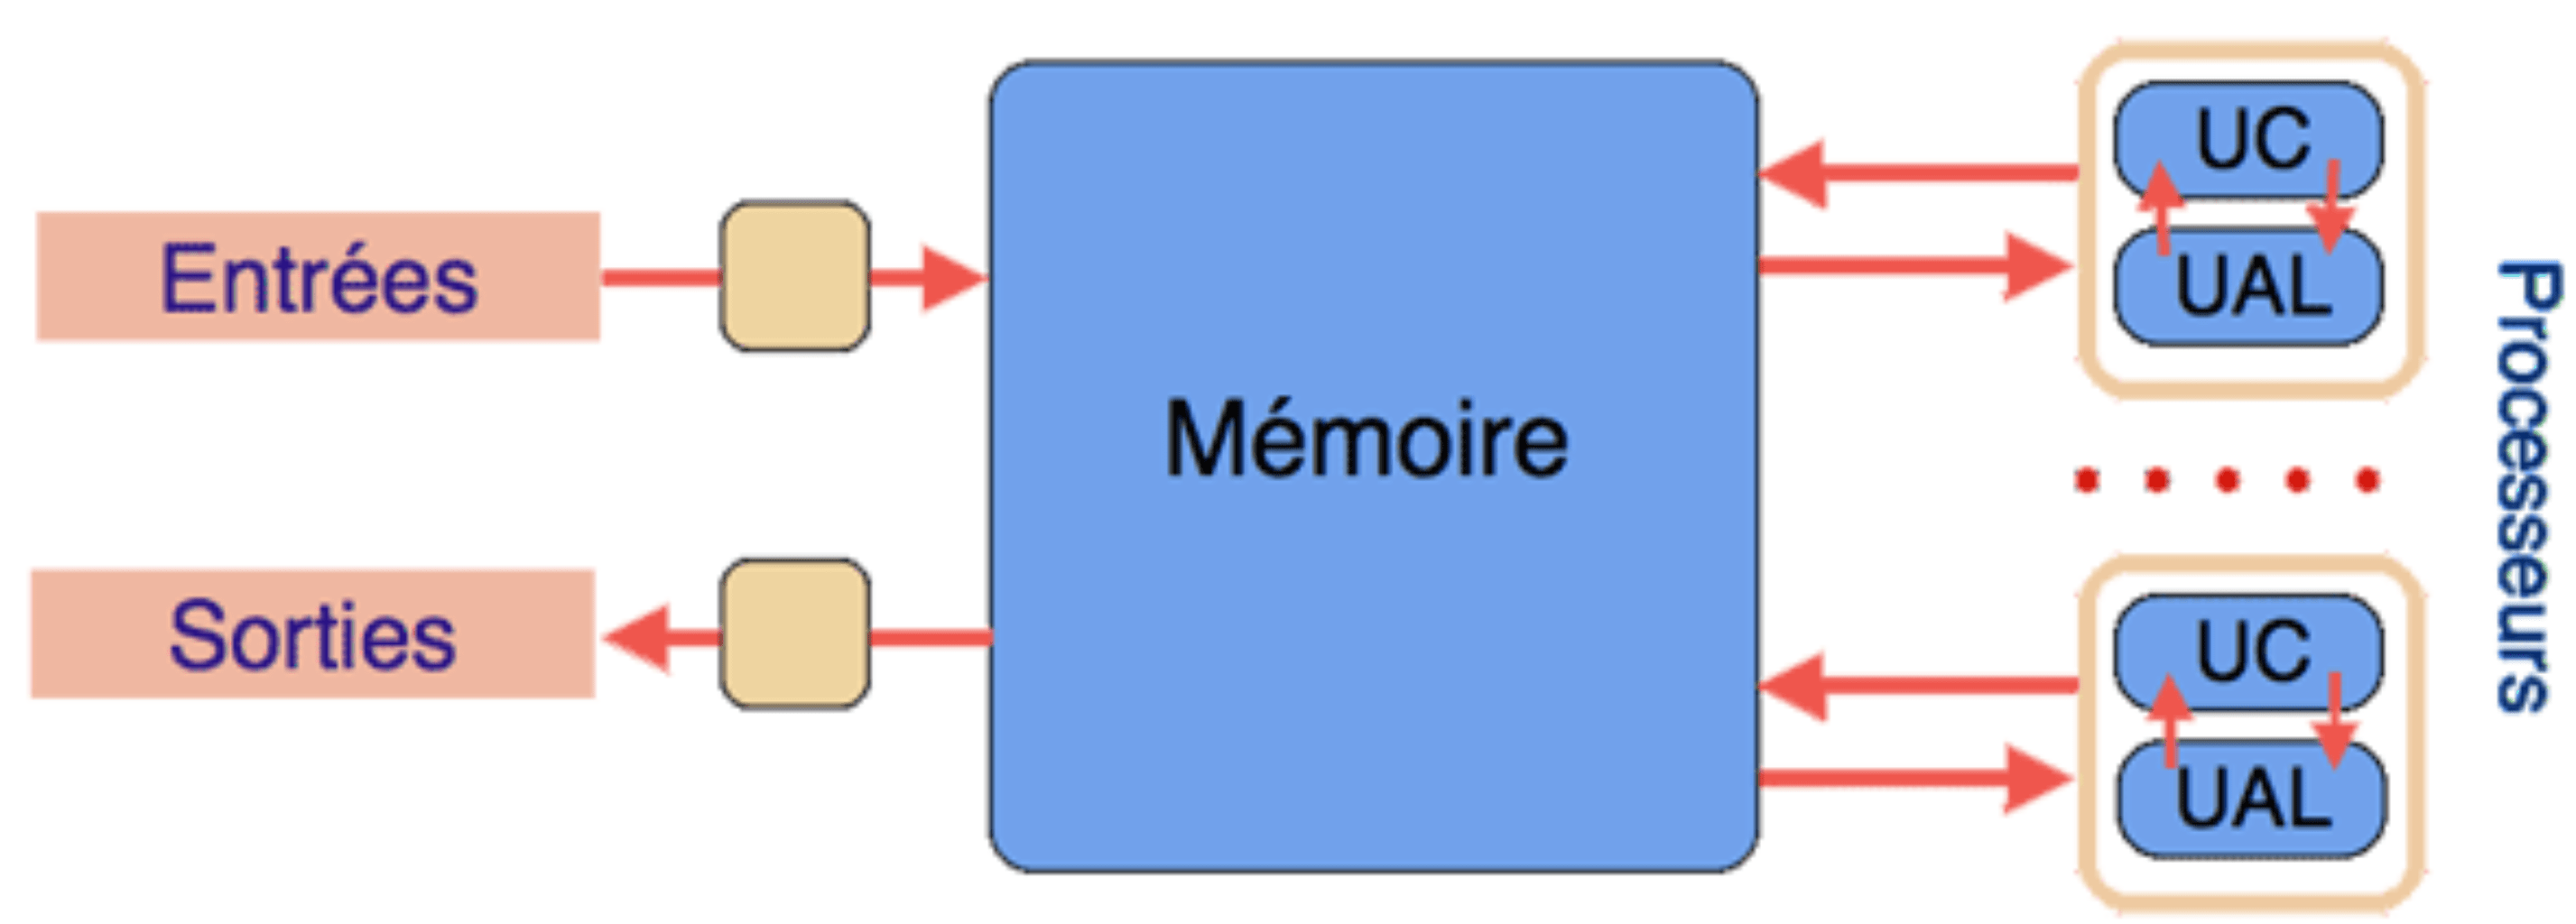
\includegraphics[width=\linewidth]{images/cpu_von_new.png}
                \caption{Quelques évolutions de l'architecture}
                \label{pic_cpu_von2}
            \end{subfigure}
            \caption{Architecture Von Neumann\protect\footnotemark }\label{fig:cpu_archi_von}
        \end{figure}
        
        \footnotetext{source: https://interstices.info/le-modele-darchitecture-de-von-neumann}
        
        Bien que l'implémentation de cette architecture ait évolué avec l'apparition de nouveaux matériaux, les architectures modernes des processeurs sont toujours construites sur ce modèle. Deux évolutions de l'architecture initiale ont cependant été appliquées (\autoref{pic_cpu_von2}). Les entrées et sorties ne sont plus gérées directement par l'unité centrale, mais par des microprocesseurs dédiés. L'unité centrale de traitement n'est plus unique depuis l'apparition des processeurs multicoeurs. Ces évolutions ne remettent pas en cause les principes de bases énoncés par Von Neumann. 


    \subsubsection{Architecture Harvard}\label{sec:harvard}

        Dans leur papier \cite{238389}, Von Neuman et al. précisent que la façon dont sont stockées les instructions et les données en mémoires doit être la même. Cette configuration la différencie de sa principale concurrente, l'architecture  Harvard (figure \ref{pic_neumannHarvard}) qui utilise deux bus pour accéder à deux mémoires réservées: l'une pour les instructions, l'autre pour les données. 
        Cette configuration permet à l'architecture Harvard d'accéder en parallèle aux données et aux instructions. De plus, comme les instructions et les données sont séparées, elles peuvent être stockées sur des supports de différentes performances. On peut ainsi utiliser un support plus cher pour stocker les données avec des mémoires très rapides (SRAM) et stocker les instructions sur des mémoires moins chers de type ROM. De plus, l'architecture Harvard apporte une sécurité en empêchant les processeurs d'exécuter des instructions provenant du stockage réservé aux données. Cependant, la nécessité d'avoir deux bus rend les puces Harvard plus chères et les performances sont souvent moins bonnes. Un code qui aurait beaucoup d'accès mémoire ne pourrait pas profiter de la disponibilité du canal allant à la mémoire des instructions. Dans une architecture Von Neumann à deux canaux, les bus peuvent être utilisés aussi bien pour des instructions que pour les données. Cependant la performance de ce bus mémoire est à l'origine du déséquilibre de performance des architectures modernes. Ainsi, il est courant d'utiliser le terme de \textit{goulot de Von Neumann} pour désigner ce point faible des architectures modernes.
        
        \begin{figure}
            \center
            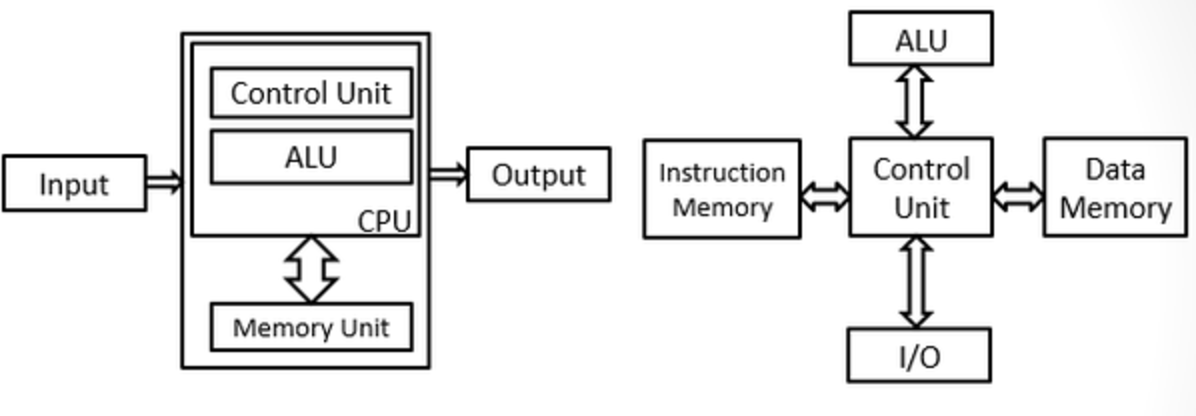
\includegraphics[width=10cm]{images/Chapitre1/neumannHarvard.png}
            \caption{\label{pic_neumannHarvard} Les deux principales architectures de processeurs: Von Neumann et Harvard. }
        \end{figure}


    \subsubsection{Performance d'une architecture}
    
    
        Le développement d'une nouvelle microarchitecture doit prendre en compte plusieurs facteurs qui peuvent impacter son implémentation (vitesse de traitement des instructions, le coût de fabrication, la fiabilité, consommation électrique, taille). Ces différents facteurs font pression sur les architectes de processeurs qui doivent redoubler d'inventivité pour les satisfaire en implémentant des optimisations matérielles.
        
        Les améliorations ont pour but d'améliorer la performance de l'architecture, la plupart du temps de façon transparente pour l'utilisateur. Cependant, un programmeur n'étant pas averti de ces optimisations, pourraient écrire des applications inefficaces, voire contre-productives. Les développeurs d'applications de \gls{HPC} étant généralement des scientifiques experts dans leur domaine (physique, chimie, mécanique…), il est fréquent de voir des codes peu efficaces. Cette section liste les principales améliorations des microarchitectures qu'il faut connaître et utiliser pour exploiter le maximum des performances disponibles. Différentes techniques ont été implémentés dans les processeurs au fil des années, rendant ces architectures très complexes. Dans le reste de cette section nous nous intéressons aux trois principaux moyens d'améliorer leur performance:
        \begin{itemize}
            \item Améliorer l'efficacité des instructions (\autoref{sec:efficacite}) 
            \item Accélérer l'exécution des instructions: (\autoref{sec:accelerer})
            \item Exécuter les instructions en parallèle: (\autoref{sec:para})
        \end{itemize}
        
        %Quand elles ne sont pas matérielles, ces différentes améliorations peuvent être réalisées par deux techniques: dynamique ou statique. Les méthodes statiques interviennent avant que le code soit exécuté. Généralement, c'est le compilateur qui les implémente lors de la génération du code. Les techniques dynamiques sont mis en oeuvre au fil des exécutions d'instructions. Elles nécessitent donc du matériel spécialisé supplémentaire et sont donc très coûteuses. La section présente les principales techniques et matériels utilisés pour l'amélioration des performances (dynamique et statique). Deux améliorations majeures sont présentées dans deux sections distinctes: la hiérarchie mémoire (\autoref{sec:hierarchie}) et la mémoire virtuelle (\autoref{sec:memoire_virtuelle}).
        
    





%%%%%%%%%%%%%%%%%%%%%%%%%%%%%%%%%%%%%%%%%%%%%%%%%%%%%%%%%%%%%%%%%%%


\subsection{Améliorer l'efficacité de l'exécution} \label{sec:efficacite}
%%%%%%%%%%%%%%%%%%%%%%%%%%%%%%%%%%%%%%%%%%%%%%%%%%%%%%%%%%%%%%%%%%%



        
    \subsubsection{Jeu d'instructions ISA } \label{sec:isa}
    %%%%%%%%%%%%%%%%%%%%%%%%%%%%%%%%%%%%%%%%%%%%%%%%%%%%%%%%%%%%%%%%%%%
    
        Le choix de l'ISA à implémenter est le premier choix à réaliser lors du développement d'une nouvelle microarchitecture. L'ISA utilisé à un impact sur la performance, la facilité de programmation et sur la compatibilité des applications existantes. Les jeux d'instructions couramment utilisés sont séparés en deux grandes familles d'ISA: les jeux d'instructions CICS pour \textit{Complex Instruction Set Computing} et les instructions RISC pour \textit{Reduced Instruction Set Computing}. La principale différence entre les deux est la complexité de leurs instructions. 
        
            \paragraph{CISC} est la première famille d'instructions à avoir été utilisée massivement. Ces instructions sont dites complexes, car une seule instruction peut à elle seule demander plusieurs opérations à réaliser. Par exemple, une addition CISC s'occuperait de charger les données depuis la mémoire, d'exécuter l'addition pour ensuite sauver le résultat. À l'origine, beaucoup de codes étaient écrits en assembleur, et ce genre d'instructions permettaient au programmeur d'éviter d'écrire de nombreuses lignes de codes souvent redondantes. De plus, les codes générés en CISC sont plus petits et nécessitent donc moins de mémoire, qui à l'origine manquait énormément.
        
            \paragraph{RISC} regroupe les ISA dites \textit{simple}. En 1970, John Cocke, alors ingénieur chez IBM, proposa de réduire le nombre d'instructions CISC \cite{cocke1990evolution}. Le terme \textit{réduit} fait référence au nombre d'instructions plus petit que celles de CISC, mais aussi pour signifier que le travail à réaliser par une instruction était moindre que pour une instruction CISC. Pour réaliser une multiplication entre deux données, on devra alors explicitement charger la première donnée, puis la deuxième et enfin écrire l'instruction qui correspond à la multiplication. Les instructions étant plus nombreuses, le travail des compilateurs est augmenté, mais souvent l'exécution des codes résultante en est réduite. Le RISC fut une réponse apportée à la lenteur de décodage du CISC.  Toutes les instructions font la même taille, les architectures nécessitent donc moins de transistors pour les analyser. Les microarchitectures sont donc moins coûteuses et peuvent atteindre des fréquences plus élevées. 
        
        
        Ces deux familles d'instructions ont toutes deux leurs avantages et leurs inconvénients et les puces actuelles comportent des parties qui exécutent des instructions RISC et d'autres en CISC. L'ISA la plus répandue est le \verb|x86| qui se veut être un jeu d'instruction CISC. Les ISA RISC les plus connus sont les ISA ARM, MIPS (utilisé dans le domaine universitaire pour apprendre le langage assembleur), PA-RISC (Hewlett-Packard) et RISC-V. L'ISA CISC la plus utilisée dans les supercalculateurs aujourd'hui est \verb|x86| (processeurs Intel et AMD).
        
        
        
        \paragraph{Extensions vectorielles.}
        
            Pour tirer partie de la puissance de calculs des processeurs et des unités de calculs vectorielles, les ISA ont reçu de nombreuses extensions (\autoref{tab_simd}).
            C'est en 1995 que Sun Microsystem introduit son premier jeu d'instruction vectoriel, le Visual Instruction Set auquel Intel répondra en 1997 avec son processeur Pentium MMX et le jeu d'instructions du même nom. Ainsi ces instructions pouvaient réaliser des opérations sur les jeux de données tels que les images ou vidéos de façon très performante. En 1997 AMD viendra améliorer le jeu d'instruction MMX avec l'implémentions des instructions 3DNow ! qui rendait alors possible les opérations vectorielles sur les nombres flottants. La possibilité de faire une opération sur deux nombres flottant par cycle doublait alors la performance des processeurs. Intel répondit alors à cette avancée avec le jeu d'instructions Streaming SIMD Extensions (SSE) en 1999. Il est alors facile d'augmenter la puissance des processeurs : il suffit d'augmenter la taille des vecteurs.
            L'ISA \verb|x86| a reçu plus de dix extensions dans les vingt dernières années pour s'adapter à l'agrandissement des unités vectorielles. Les principales sont \textit{MMX} (1996), \textit{3DNOW!} (1998), 6 versions de \textit{SSE} de 1999 2008 et enfin \textit{AVX-2} et \textit{AVX-512} en 2013 et 2015. Évidemment, les codes ne peuvent pas profiter de ces instructions sans une microarchitecture capable de les exécuter. Ces microarchitectures sont présentes dans la sous-section suivante. 
        
                % Please add the following required packages to your document preamble:
                % \usepackage{graphicx}
                \begin{table}[]
                \centering
                %\resizebox{\textwidth}{!}{%
                \begin{tabular}{|l|l|l|l|l|l|}
                \hline
                \multicolumn{1}{|c|}{Année} & \multicolumn{1}{c|}{Nom} & \multicolumn{1}{c|}{Nb registres} & \multicolumn{1}{c|}{Taille (bit)} & \multicolumn{1}{c|}{Registres} & \multicolumn{1}{c|}{Commentaires} \\ \hline
                1996 & MMX & 8 & 64 & MM0 & Nombre entiers \\ \hline
                1999 & SSE & 8 & 128 & XMM0 & 120 instr., simple precisions \\ \hline
                2006 & SSSE3 & 8 & 128 & XMM0 & 300 instr., double précisions \\ \hline
                2008 & AVX & 16 & 128 & XMM0 & FMA4, op. a 3 opérandes \\ \hline
                2011 & AVX2 & 16 & 256 & YMM0 &  \\ \hline
                2013 & AVX512 & 32 & 512 & ZMM & FMA3 \\ \hline
                \end{tabular}%
                %}
                \caption{Évolutions principales des instructions SIMD \texttt{x86}}
                \label{tab_simd}
                \end{table}

        
            \begin{figure}
                \center
                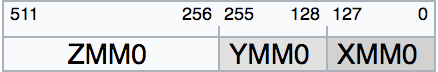
\includegraphics[width=7cm]{images/Chapitre1/simd_registres.png}
                \caption{\label{pic_simd_registres} Découpage d'un registre de 512 bits}
            \end{figure}

    \subsubsection{Les processeurs vectoriels } \label{sec:cpu_vectoriel}
    %%%%%%%%%%%%%%%%%%%%%%%%%%%%%%%%%%%%%%%%%%%%%%%%%%%%%%%%%%%%%%%%%%%

        Dans les années 90, les ordinateurs personnels commençaient à être utilisés pour le multimédia (film, image, musique). Dans le but d'augmenter la performance des applications, les architectes ont voulu améliorer l'efficacité des instructions en implémentant des architectures SIMD (Single Instruction Multiple Data de la taxonomie de Flynn présentée dans la \autoref{sec:prog_parallele}). 
        
        L'architecture vectorielle repose sur les mêmes fondements que l'architecture superscalaire (voir \autoref{sec:superscalar}): réduire le temps d'exécution d'un code en utilisant le parallélisme et diminuer le coût en transistors de la microarchitecture par la mise en commun du matériel entre plusieurs unités de calculs (\autoref{pic_cpu_simd}). La pression que subit l'unité responsable du \textit{fetch} et du \textit{decode} est donc réduite, car avec une seule instruction vectorielle, le processeur réalise le travaille de plusieurs instructions scalaires.  Contrairement au processeur scalaire qui exécute une instruction sur une seule donnée, les processeurs vectoriels sont capables d'exécuter une instruction sur plusieurs données simultanément (\autoref{pic_simd2}).
        
        \begin{figure}[ht!]
        \centering
        \begin{subfigure}[t]{0.48\textwidth}
            \centering
            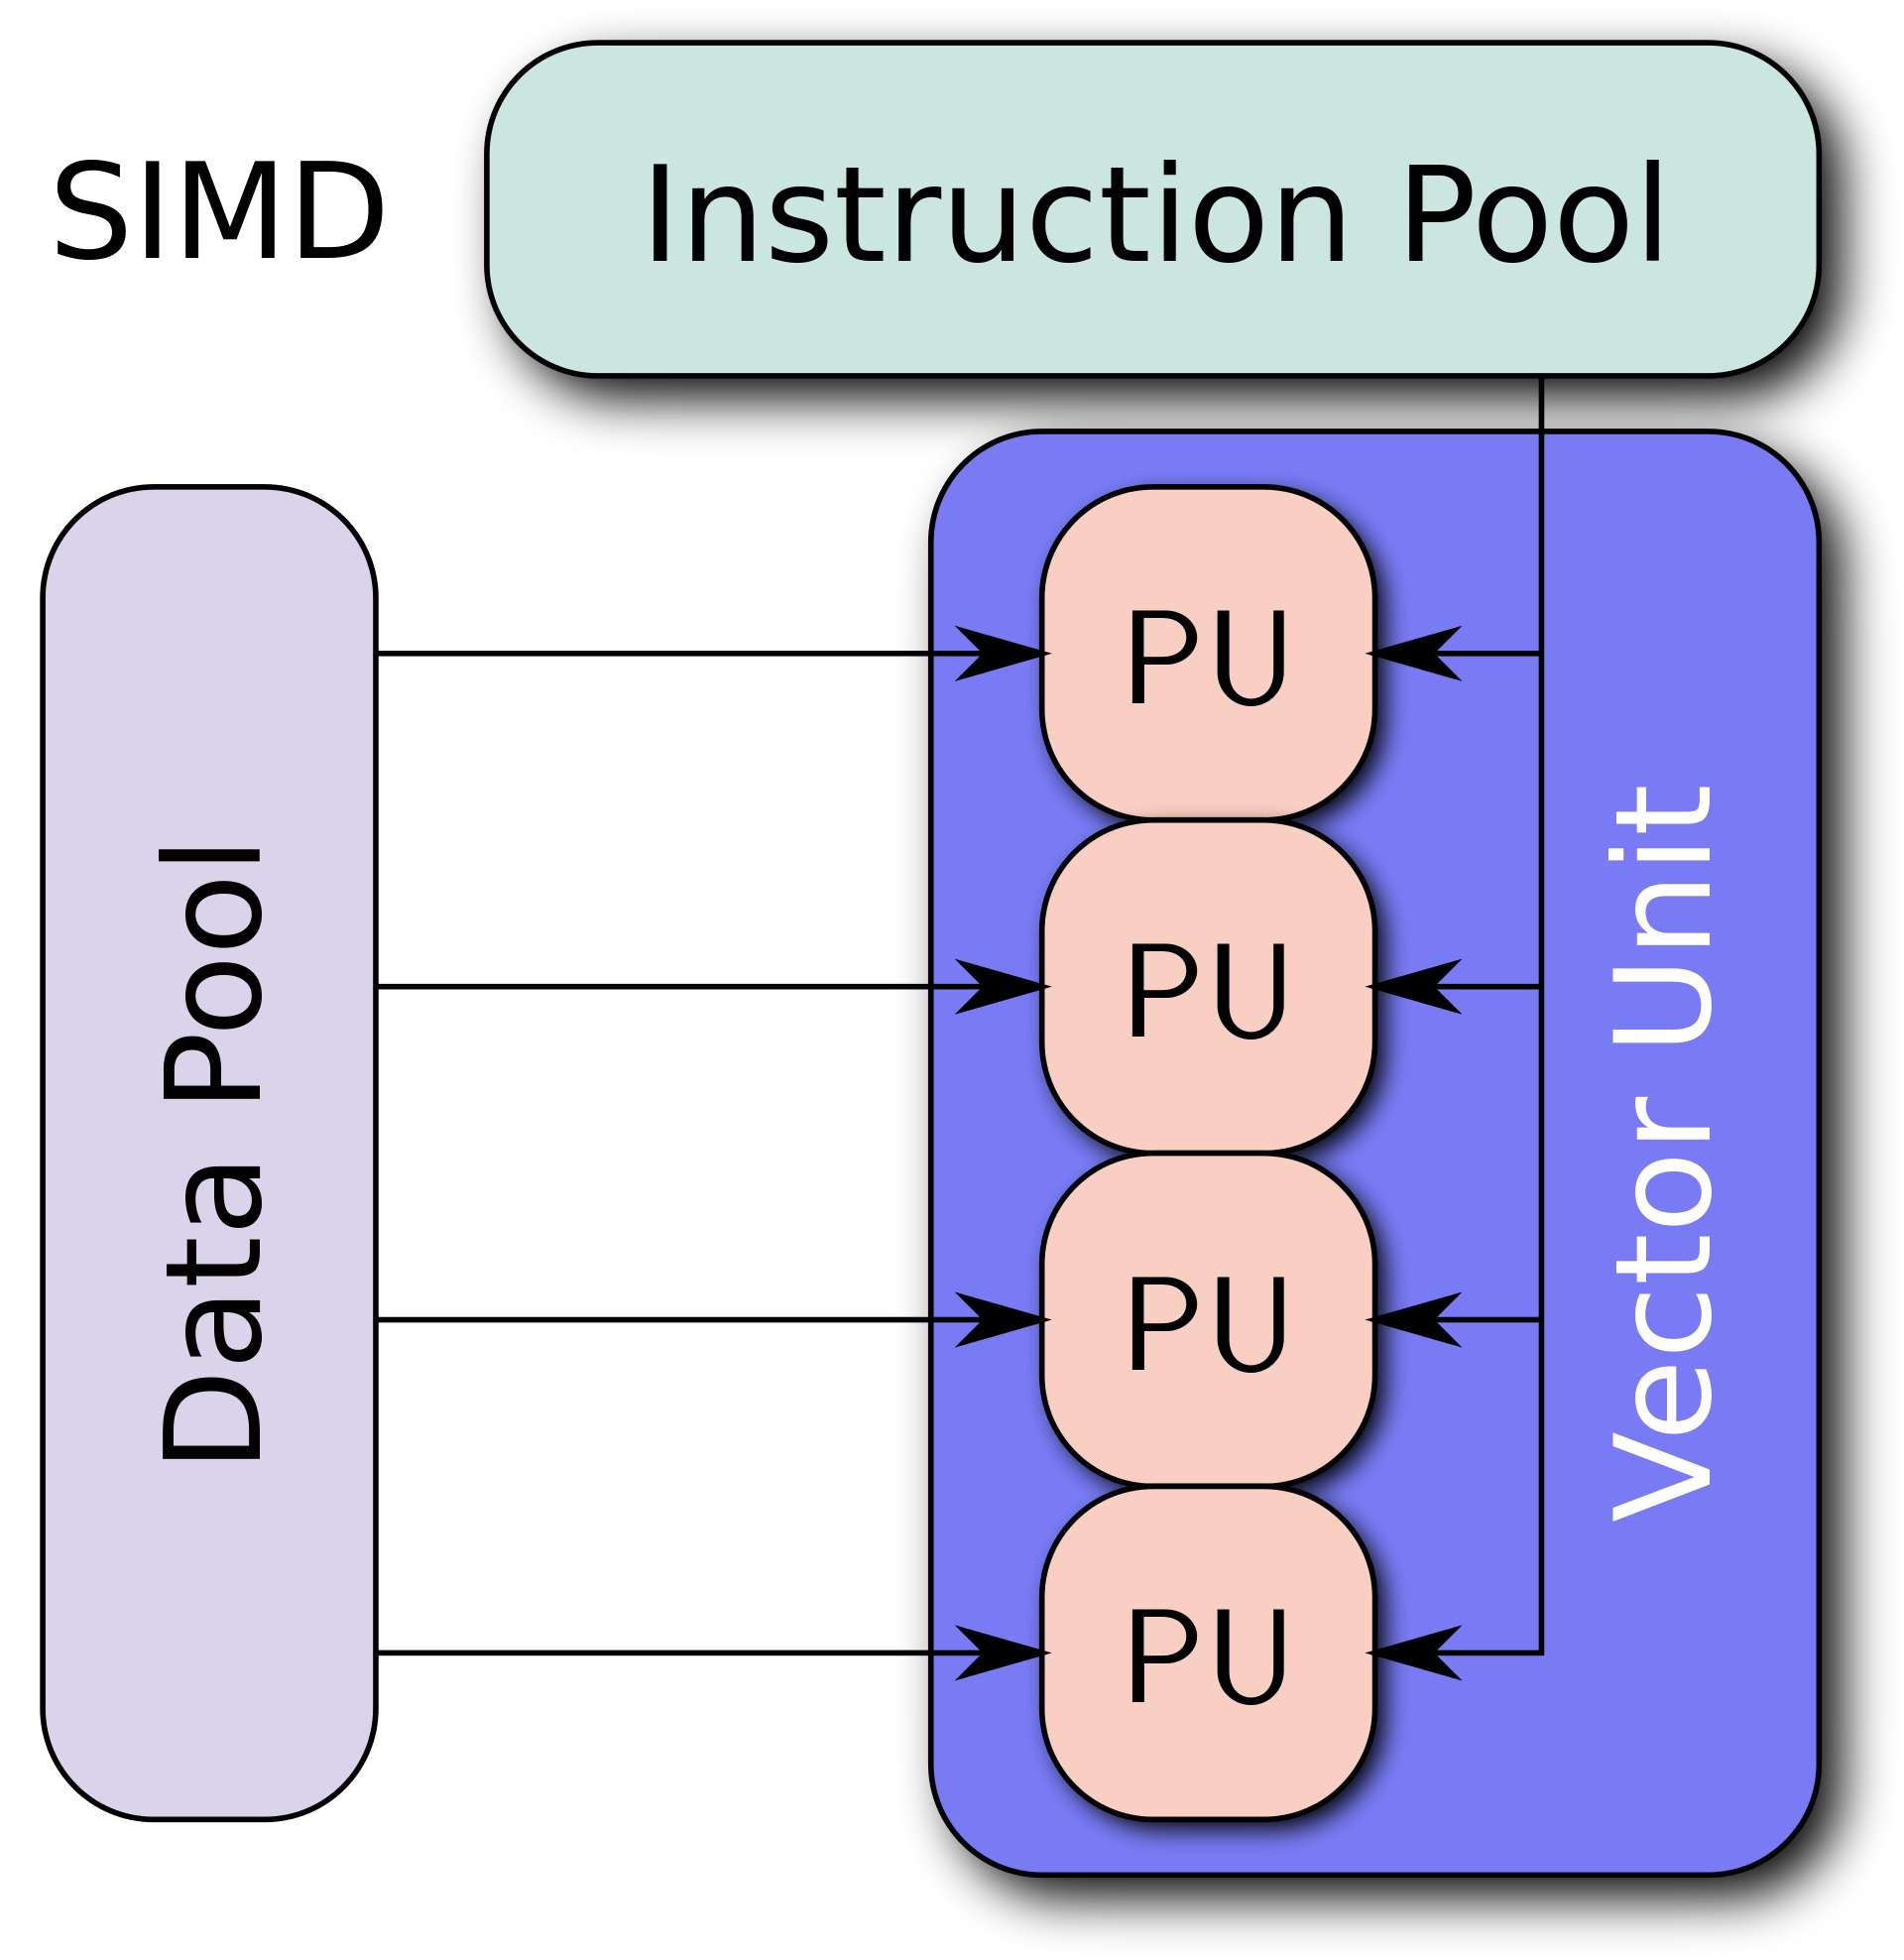
\includegraphics[width=.45\linewidth]{images/cpu_simd.png}
            \caption{Un processeur vectoriel exécute une même instruction sur différentes données
                \label{pic_cpu_simd}}
        \end{subfigure}\hfill
        \begin{subfigure}[t]{0.48\textwidth}
            \centering
            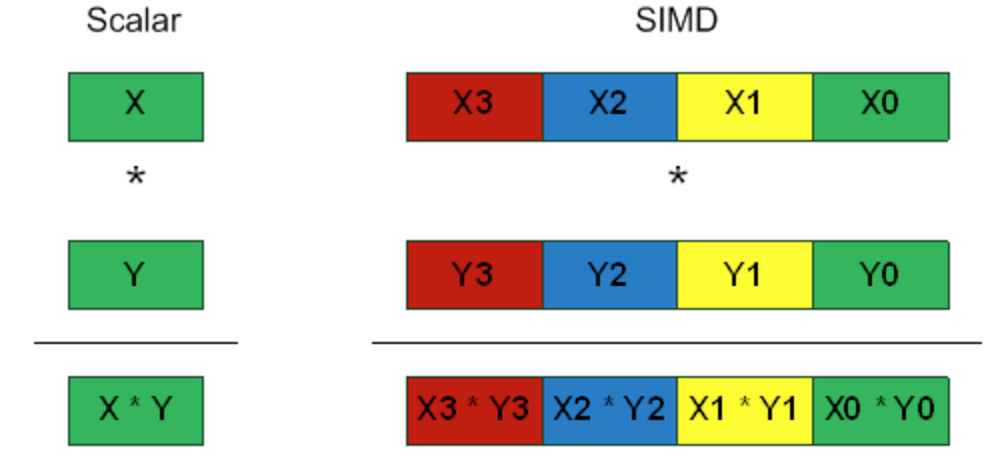
\includegraphics[width=\linewidth]{images/Chapitre1/simd.png}
            \caption{Schéma de fonctionnement d'une multiplication vectorielle\protect\footnotemark}
                \label{pic_simd2}
        \end{subfigure}
        \caption{Un processeur vectoriel travaille sur un groupe de données indépendantes. Les opérandes sont alors stockées dans des registres vectoriels capable de charger un vecteur pour y appliquer une même opération.}
                    \label{pic_simd}
        \end{figure}
        \footnotetext{source:\url{https://software.intel.com/en-us/articles/ticker-tape-part-2}}


        
        Ainsi, doubler la largeur des instructions revient à doubler le nombre de \gls{FLOP} réalisables par le processeur alors que la consommation électrique augmentera d'un facteur inférieur à 2. Beaucoup d'efforts ont donc été réalisés pour être capables d'utiliser cette technologie. Par exemple la majorité des compilateurs est capable de détecter les zones de codes parallélisable pouvant bénéficier d'instructions SIMD.
        Cependant, dans la pratique les codes ne sont pas aussi parallèles que nous le souhaiterions et certains aspects du code empêchent de tirer la totalité de la performance disponible. En effet, si les instructions sont dépendantes les unes des autres, il est alors impossible de les calculer simultanément rendant la partie vectorielle inutilisable. Aussi, les performances peuvent être réduites si les données accédées ne sont pas continues en mémoire. Cela demande donc un travail supplémentaire pour repenser les structures de données et s'assurer que les donnes transférées sur le bus mémoire sont des données utiles (voir le concept de ligne de cache dans la \autoref{sec:cache}).



\subsection{Accélérer l'exécution des instructions} \label{sec:accelerer}
%%%%%%%%%%%%%%%%%%%%%%%%%%%%%%%%%%%%%%%%%%%%%%%%%%%%%%%%%%%%%%%%%%%

    Utiliser des instructions plus efficaces telles que les instructions vectorielles ou les FMA est un premier moyen d'améliorer la puissance de calcul d'un processeur. Un deuxième moyen est de les exécuter plus rapidement. Cela peut être réalisé en accélérant la fréquence d'un processeur, ou en utilisant des matériels spécialisés pour l'exécution de ces instructions.

    \subsubsection{Lien entre fréquence et performance} \label{sec:frequency}

        Les processeurs sont des circuits électroniques dits \textit{synchrones}. Leur fonctionnement est cadencé par une horloge donnant des impulsions régulières aux composants du circuit pour organiser leur synchronisation. Lorsqu'une instruction est exécutée par le processeur les passages dans les différentes étapes de la microarchitecture, notamment du pipeline (voir \autoref{sec:pipeline}), sont régis par cette horloge. Au plus l'horloge est rapide, au plus l'exécution du programme l'est aussi. Cependant, la durée séparant deux signaux (un cycle) ne peut pas être réduite à l'infini. En effet, les vitesses d'horloges sont si rapides, qu'il est nécessaire de laisser suffisamment de temps au signal électrique de se propager dans le circuit. La taille du processeur et sa fréquence sont donc liées, c'est notamment pour cette raison qu'il n'existe pas de processeur mesurant plusieurs dizaines de centimètres. À une fréquence de 3 GHz, le signal électrique, qui se déplace à la vitesse de la lumière, ne peut parcourir que quinze centimètres entre deux cycles. En plus du temps de propagation, il faut aussi prévoir le temps de préparer et recevoir la communication. L'augmentation de la fréquence des processeurs a donc une première limite physique infranchissable bien que d'autres limites présentées dans cette partie soient encore plus contraignantes.
        
        La fréquence des processeurs a beaucoup évolué depuis les premiers processeurs (\autoref{pic_cpu_frequency}). Les premiers processeurs \textit{Pentium} d'Intel utilisaient des fréquences de 60 MHz en 1993. Pendant plus de dix ans, les fréquences ont évolué chaque année d'un facteur de 40\%  tous les ans pour atteindre des vitesses de plusieurs Gigahertz. En 2000, Intel annonçait la fabrication de processeurs cadencés à 10 GHz\footnote{source \url{https://www.clubic.com/actualite-1791-des-processeurs-intel-10-ghz-pour-2005.html}} pour les années 2005. Pourtant, en 2019, nous sommes encore loin d'utiliser des processeurs avec de telles cadences. Mis à part les systèmes surcadencés, utilisant des systèmes de refroidissement liquide, il est rare de voir des systèmes utiliser des processeurs récents à plus de 5 GHz.
        .
        \begin{figure}
            \center
            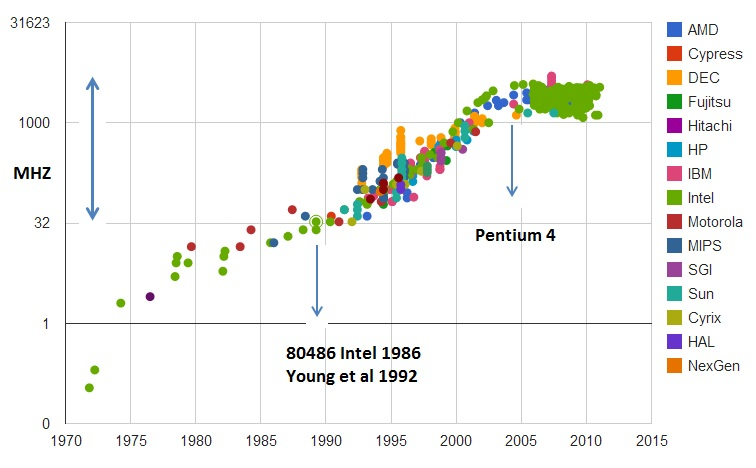
\includegraphics[width=14cm]{images/cpu_frequency.jpg}
            \caption{\label{pic_cpu_frequency} Évolution de la fréquence des processeurs\protect\footnotemark.}
        \end{figure}
        \footnotetext{source: \url{https://en.wikipedia.org/wiki/Beyond_CMOS}}
        
        Le but de cette section est de comprendre pourquoi l'évolution de la fréquence des processeurs s'est arrêtée brusquement autour des 4 GHz. Pour cela, nous expliquons comment la loi de Moore a permis d'en arriver là, et quelles sont les limites physiques qui empêchent de poursuivre cette évolution.


    \subsubsection{Loi de Dennard}\label{sec:denard}

        Comme constaté dans la section précédente, la fréquence de l'horloge d'un processeur est limitée par le temps nécessaire au signal de se propager entre deux éléments d'un circuit. Plus les transistors seront proches, plus la vitesse de propagation sera faible. La loi de Moore prévoit que le nombre de transistors double tout les deux ans pour une surface donnée. Cela est rendu possible par l'affinement de la gravure permettant de réaliser des transistors toujours plus petits et donc plus proches. Avec plus de transistors, les processeurs peuvent utiliser des pipelines plus complexes, entre divisant les étapes les plus longues permettant aussi l'utilisation de fréquence plus élevée. Nous expliquons comment l'évolution de la fréquence des processeurs est intimement liée avec la loi de Moore en utilisant la formule de la consommation électrique d'un circuit CMOS \cite{martin2014post}:
        \begin{equation}
        P = QfCV^{2} +  VI_{leakage}
        \label{eq:power}
        \end{equation}
        
        
        L'intérêt de cette formule est d'apprécier comment la puissance et la fréquence d'un processeur est impactée par la loi de Moore. Pour cela, nous étudions sa variation entre deux générations de processeurs, c'est-à-dire une période de deux ans
        \begin{itemize}
        
            \item \textbf{Le nombre de transistors $Q$ : } D'après la loi de Moore, le nombre de transistors double tous les deux ans pour deux circuits de mêmes surfaces. Ainsi la surface des transistors est divisée par deux. Leur longueur et  leur largeur est ainsi réduite d'un facteur $\sqrt{2}$. Cette valeur est appelée facteur de \textit{scaling} et a une valeur de $1.44$.
            
            \item \textbf{La capacité du circuit $C$ : } La capacité d'un transistor peut être calculée par la formule suivante $C = \frac{S \times e}{d}$. Avec $S$ la surface du transistor, $e$ la permittivité électrique du matériau utilisé (pouvant être considéré comme fixe entre deux générations), et $d$ la distance séparant la grille et le semi-conducteur (isolant). Comme vu précédemment, la surface $S$ d'un transistor est divisé par $2$ entre deux générations. La distance $d$ est-elle réduite par un facteur $\sqrt{2}$. Tous les deux ans, la capacité d'un transistor est donc réduite d'un facteur $\sqrt{2}$. 
            
            \item \textbf{La fréquence du circuit $f$ : } La fréquence d'utilisation d'un transistor dépend essentiellement de la vitesse à laquelle la grille peut être chargée ou déchargée. Diminuer sa capacité diminue du même facteur ce temps de remplissage. Entre deux générations, la fréquence est supposée augmenter d'un facteur $\sqrt{2}$. Cette valeur correspond bien à l'augmentation de $40\%$ constatée dans l'introduction de cette section. 
            
            \item \textbf{La tension de fonctionnement $V$ : } La tension est proportionnelle à la finesse de grave utilisée. Diviser la finesse de gravure par un coefficient de $\sqrt{2}$ revient à diviser la tension de fonctionnement par le même facteur. 
            
            \item \textbf{Les courants de fuites $I_{leakage}$ : } Les courants de fuites sont considérés comme négligeables (pour le moment). 
        
        
        \end{itemize}
        
        
        \paragraph{Variation de $P$.} À une tension de fonctionnement $V$ égale entre deux générations de processeurs et en reprenant les variations des différentes valeurs, nous constatons que $P$ ne varie pas entre deux générations. Le \autoref{tab:dennard} résume les différents impacts que la diminution de la finesse de gravure à sur les différentes propriétés d'un circuit. On remarque deux choses concernant l'évolution de $P$ entre deux générations de circuit. La première est que l'augmentation de la fréquence est compensée par la baisse de la capacité du circuit. La deuxième est que la baisse de tension compense le nombre de transistors. Ainsi, la consommation électrique d'un processeur ne varie pas entre deux générations, bien que la fréquence augmente de $40\%$ et que le nombre de transistors soit doublé. Cette propriété est connue sous le nom de Loi de Dennard \cite{Dennard1974} qui assurait en 1974 que la densité énergétique resterait constante entre deux générations de processeurs. Cette propriété est restée vraie durant 30 ans, permettant l'augmentation de la performance des processeurs sans augmenter drastiquement leur consommation électrique. 
        
        % Please add the following required packages to your document preamble:
        % \usepackage{graphicx}
        % \usepackage[table,xcdraw]{xcolor}
        % If you use beamer only pass "xcolor=table" option, i.e. \documentclass[xcolor=table]{beamer}
        \begin{table}[]
        \centering
        \resizebox{\textwidth}{!}{%
        \begin{tabular}{lc}
        \hline
        \rowcolor[HTML]{EFEFEF} 
        {\color[HTML]{000000} Paramètre} & {\color[HTML]{000000} Coefficient multiplicateur (tous les deux ans)} \\ \hline
        Finesse de gravure & $\frac{1}{\sqrt{2}}$ \\
        Nombre de transistors par unité de surface & $2$ \\
        Tension d'alimentation & $\frac{1}{\sqrt{2}}$ \\
        Capacité d'un transistor & $\frac{1}{\sqrt{2}}$ \\
        Fréquence & $\sqrt{2}$ \\ \hline
        \end{tabular}%
        }
        \caption{ Résumé des impacts de la diminution de la finesse de gravure d'un facteur $\sqrt{2}$\protect\footnotemark.}
        \label{tab:dennard}
        \end{table}
        
        \footnotetext{source: \url{https://fr.wikibooks.org/wiki/Fonctionnement_d\%27un_ordinateur/La_consommation_d\%27\%C3\%A9nergie_d\%27un_ordinateur}}
        
        




    \subsubsection{Fin de Dennard}

        Les équations de Dennard se sont appliquées pendant plus de 30 ans, voyant la fréquence des processeurs augmenter de 40\% tous les 2 ans (voir \autoref{pic_cpu_evolution}). Cependant, l'\autoref{eq:power} ignorait les courants de fuite $I_{leakage}$ alors peu significatifs. Avec la miniaturisation des transistors, ces fuites augmentent exponentiellement pour des tailles de gravure inférieures à 65nm \cite{martin2014post}. Alors que la loi de Dennard prévoyait une consommation électrique constante entre deux générations de processeur, ces fuites de courant vont faire augmenter la consommation des puces d'un facteur 2. Ceci entraîne une forte évolution de la densité électrique à chaque nouvelle génération (voir \autoref{pic_cpu_leakage}) impactant la consommation électrique des processeurs (voir \autoref{pic_cpu_evolution}). Au plus la fréquence des processeurs est élevée, au plus les transistors sont activés augmentant d'autant les courants de fuite. La chaleur dégagée par les puces n'est alors plus soutenable et l'évolution de la fréquence des processeurs s'arrête ainsi autour des années 2005.
        
        \begin{figure}
            \center
            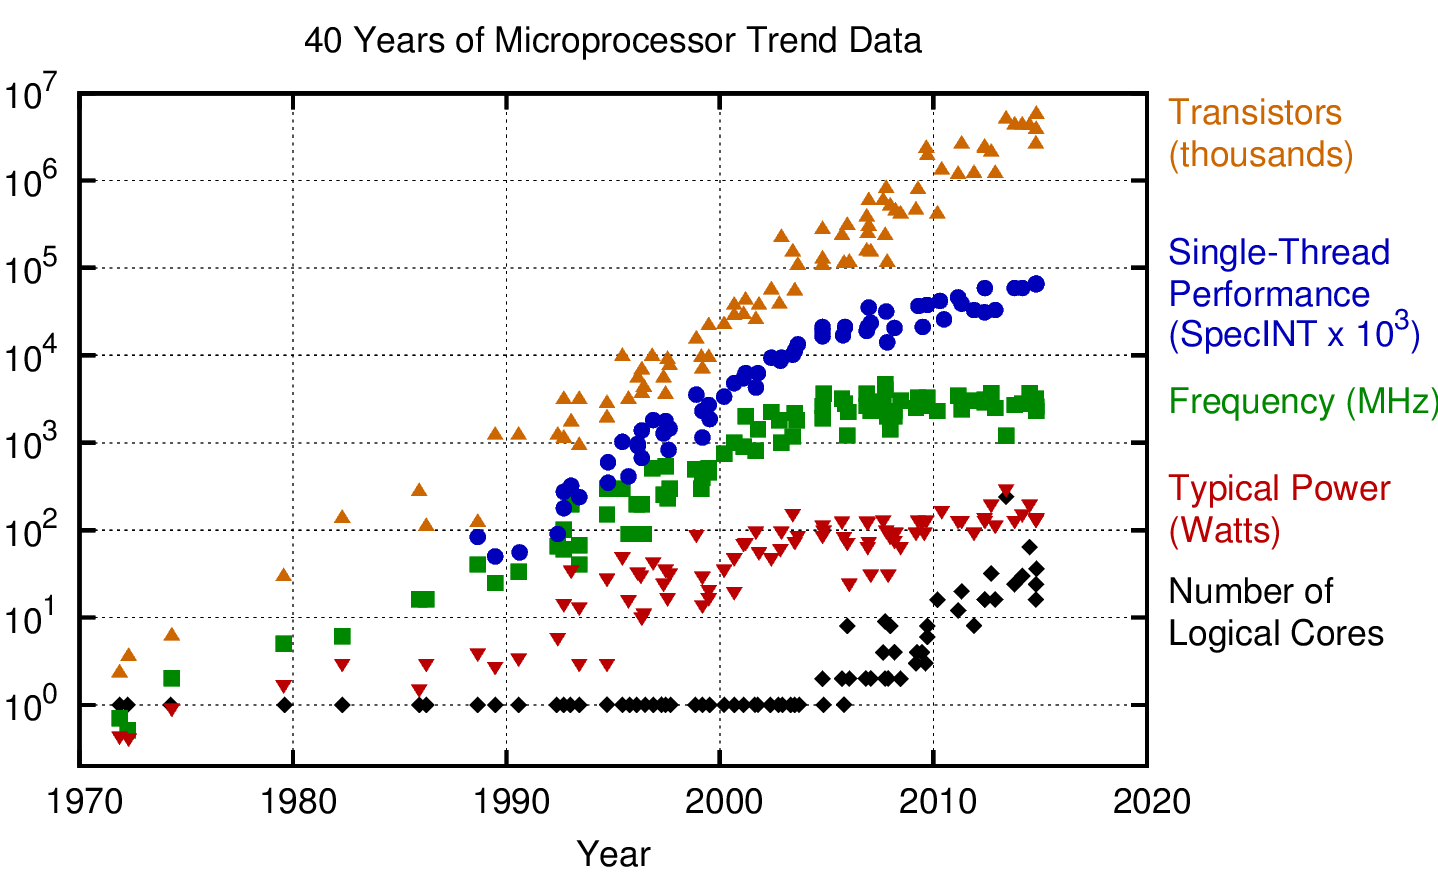
\includegraphics[width=10cm]{images/cpu_evolution.png}
            \caption{\label{pic_cpu_evolution} Évolution des caractéristiques des processeurs \cite{rupp40years}.}
        \end{figure}
        
        \begin{figure}
            \center
            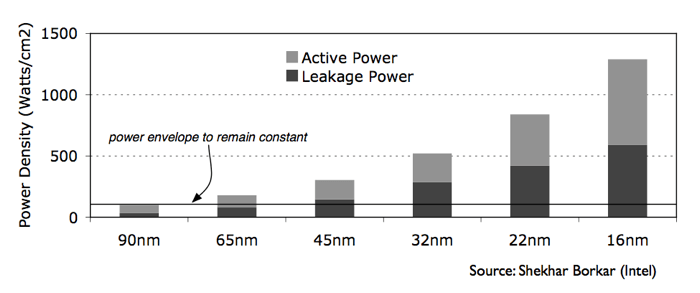
\includegraphics[width=10cm]{images/cpu_leakage.png}
            \caption{\label{pic_cpu_leakage} La miniaturisation de l'isolant nécessaire au fonctionnement des transistors permet le passage de courant de \textit{fuites}.}
        \end{figure}
        
        Bien que la fréquence des processeurs n'augmente plus depuis plus de 10 ans, la \autoref{pic_cpu_evolution} montre que la performance des processeurs continue bien d'augmenter. En effet, si la loi de Dennard n'est plus valide, la loi de Moore l'est encore après 2005. Les processeurs reçoivent toujours plus de transistors permettant d'augmenter la complexité des pipelines. Ces transistors sont alors utilisés pour construire des processeurs avec plusieurs coeurs. Présentés dans la \autoref{sec:multicore}, il est intéressant de remarquer que l'augmentation du nombre de coeurs commence exactement quand la fréquence n'augmente plus. Les processeurs sont alors capables de réguler la chaleur d'un processeur en plaçant les processus peu actifs sur les points chauds de la puce.
        Pour limiter la consommation électrique, des techniques de management d'alimentation sont alors mises en place pour éteindre certaines parties du processeur inutilisées.
        L'utilisation de différentes fréquences est aussi largement utilisée. Les processeurs possèdent des fréquences dites \textit{turbo}, leur permettant d'atteindre des fréquences très élevées pendant un court laps de temps ou lorsque le processeur n'est pas pleinement utilisé (coeurs et calculs vectoriels inutilisés).



    \subsubsection{FPU}\label{sec:fpu}
        
        Le second moyen d'accélérer l'exécution des instructions est d'utiliser des matériels spécialisés pour leur exécution. L'unité de calcul en virgule flottante (\gls{FPU}) est un composant du processeur permettant de réaliser les opérations sur les nombres à virgule flottante. À l'origine ce module était séparé du processeur et il convenait à l'utilisateur de choisir s'il voulait ou non en brancher une sur la carte mère dans l'emplacement qui lui était alors dédié. Pour des questions de coûts d'intégration et de performance, la FPU est depuis 1989, avec la sortie du processeur Intel 80486,  intégrée au processeur. 
        
        Au fil des années, la complexité de la FPU a augmenté. Quand elle n'était capable d'exécuter que de simples opérations à l'origine, elle peut désormais réaliser des opérations complexes (division, racine carrée, exponentielles ou des fonctions trigonométriques).  De plus, des instructions fusionnées ont fait leur apparition en 2013 dans les processeurs \textit{Haswell} de Intel et Piledriver pour AMD. Elles ont la particularité de réaliser 2 opérations en un seul cycle d'horloge du processeur. Connues sous le nom de FMA pour \textit{fused multiply-add} elles sont capables d'exécuter l'instruction $a \leftarrow b * c + d$ en un seul cycle. 
        
        Enfin, les unités de calcul modernes sont capables d'exécuter une opération sur plusieurs données à la fois. Ce type d'instructions est dit \textit{vectoriel}. Ces instructions sont performantes pour les algorithmes qui doivent exécuter une même opération sur plusieurs données (un vecteur par exemple).
        Les différentes évolutions de la FPU sont responsables de la forte augmentation de la puissance de processeur. En effet, usuellement la puissance d'un processeur est donnée par le nombre de calculs flottant qu'il peut exécuter par cycle. Le tableau \ref{tab_FPU} montre comment le nombre de FLOP par cycle évolue: pour Intel, cette performance a été multipliée par deux à chaque nouvelle version de l'architecture et les FPU modernes exécutent 8 fois plus de calculs qu'en 2008.
        
        \begin{table}[]
        \centering
        \label{my-label}
        \begin{tabular}{|l|l|l|l|l|l|}
        \hline
        \multicolumn{1}{|c|}{\textbf{Année}} & \multicolumn{2}{c|}{\textbf{Architecture Intel / AMD}}     & \multicolumn{1}{c|}{\textbf{Simpe p.}} & \multicolumn{1}{c|}{\textbf{Double p.}} & \multicolumn{1}{c|}{\textbf{Opérations}} \\ \hline
        2008                                 & Nehalem                          & K10                     & 8                                      & 4                                       & 4 add. et 4 mul.         \\ \hline
        2011                                 & Sandy Bridge                     & Bulldozer               & 16                                     & 8                                       & 8 add. et 8 mul.         \\ \hline
        2013                                 & Haswell \& Skylake               &                         & 32                                     & 16                                      & 8 FMA (mult. + add.)        \\ \hline
        2016                                 & Xeon Phi KNL &                         & 64                                     & 32                                      & 8 FMA (mult. + add.)        \\ \hline
        \end{tabular}
        \caption{Evolution de la performance des FPU}

        \label{tab_FPU}
        \end{table}
        
        %\textbf{TODO} latence des differentes instructions; skylake FMA 4 cycles %http://agner.org/optimize/blog/read.php?i=415 (calc_fma() combien de FMA en parallele)
        
        





    \subsubsection{Optimisations}

        Dans les sous-parties précédentes nous avons présenté comment l'évolution de la fréquence et l'utilisation de matériel spécialisé comme une FPU permet d'accélérer l'exécution d'une instruction. Pour différentes raisons (dépendance, manque d'un opérande), les instructions ne peuvent pas être exécutées à la vitesse maximale théorique prévue par le processeur. Pour maximiser le nombre d'instructions exécutées chaque cycle, les processeurs ont reçu de nombreuses optimisations. 

        \paragraph{Exécution dans le désordre.}\label{sec:out_of_order}
         
        
            Le but de cet optimisation est de cacher l'attente de donnée du processeur de la mémoire. Cette avancée est apparue sur les processeurs Intel en 1995 avec le \textit{Pentium P6}. Le principe de l'exécution dans le désordre est d'exécuter les instructions dans un ordre différent que celui donné par le code source.  Ainsi lorsqu'une instruction doit attendre une donnée, au lieu de perdre plusieurs cycles à attendre ces données, le processeur va exécuter les instructions qui suivent et finira d'exécuter la première quand la donnée sera chargée dans un registre. 
            Cependant, ne pas exécuter le programme dans l'ordre initial peut fausser les résultats. C'est alors au processeur de s'assurer que les instructions permutées ne sont pas dépendantes. Il existe trois types de dépendances. 
            \begin{itemize}
                \item La première est une \textit{lecture après écriture} (Read After Write ou RAW): une instruction lit une donnée écrite par une instruction la précédent. 
                \item La deuxième est une \textit{écriture après lecture} (WAR): une première instruction lit une donnée qui est modifiée par une instruction la suivant. 
                \item La dernière dépendance est une \textit{écriture après écriture} (WAW): deux instructions écrivent sur la même donnée.  
            \end{itemize}
            Pour éliminer ces deux dernières dépendances, les processeurs possèdent plus de registres que ceux adressables par le programme. Il les utilise pour éliminer les dépendances WAR et WAW grâce à des techniques de renommage de registres \cite{903248}. L'\autoref{code_dependances} donne un exemple pour chaque type de dépendances. Dans chaque cas, la valeur de B n'est pas la même si les deux assignations ne sont pas exécutées dans le même ordre, suivant cet ordre, B peut valoir 10 ou 15. Pour ce faire, le processeur possède une fenêtre de plusieurs instructions, aussi appelée (à tord) l'\textit{execution queue}. En effet, cette liste n'a pas vocation à être exécutée dans l'ordre, c'est un rassemblement d'instructions qui ont des dépendances entre elles. Le processeur vient mettre à jour cette liste pour essayer d'exécuter des instructions qui n'ont plus de dépendances avec une donnée ou une autre instruction.
            Pour pouvoir bénéficier de l'exécution dans le désordre, le processeur doit donc détecter si les instructions sont dépendantes pour pouvoir les réordonner. Aussi, le programmeur peut aider le processeur dans son travail en évitant au maximum les dépendances entre les instructions. 
            La complexité apportée par le système d'exécution dans le désordre, peut être la source d'attaque comme la récente faille \textit{Meltdown} des processeurs Intel \cite{DBLP:journals/corr/abs-1801-01207}.
            
            
            
            \begin{lstlisting}[language=C, caption=Exemples de dépendances entre deux instructions., float,floatplacement=H, label=code_dependances]
            //----------- Read after Write -----------
            int A, B = 0
            A = 5;
            B = A + 10;
            //Result: B == 10 ou B == 15
            
            //----------- Write after Read -----------
            int A, B = 0
            B = A + 10;
            A = 5;
            //Result: B == 10 ou B == 15 
             
            //----------- Write after Write -----------
            int B = 0
            B = 10;
            B = 15;
            //Result: B == 10 ou B == 15
            \end{lstlisting}






        \paragraph{Prédiction de branchement}\label{sec:branch_predictor}

            L'exécution dans le désordre fonctionne tant que suffisamment d'instructions sont disponibles pour être exécutées. Cependant, lorsqu'un programme contient un branchement conditionnel, le processeur doit attendre que sa condition soit testée. Si cette condition utilise une variable modifiée dans les instructions précédentes, le processeur doit attendre d'avoir le résultat du test pour connaître les futures instructions à exécuter. Pour maximiser l'utilisation du pipeline, le processeur peut essayer de prédire le résultat du test et ainsi continuer l'exécution. S'il s'est trompé sur la prédiction, il doit alors annuler les instructions déjà exécutées et reprendre l'exécution des autres instructions. Le temps nécessaire pour la reprise de l'exécution après une mauvaise prédiction dépend donc de la taille du \textit{pipeline} utilisé (plusieurs dizaines de cycles).
            La prédiction de branchement peut être implémentée par deux méthodes.
            Le processeur peut posséder un matériel spécifique, appelé prédicteur de branchement (\textit{branch predictor}), qui utilise des méthodes de statistiques. Lorsqu'un branchement est faux plusieurs fois de suite, il peut estimer qu'il y a une grande probabilité qu'il le soit aussi à l'itération suivante et éviter d'attendre le résultat du test pour continuer l'exécution. Le processeur peut aussi, à partir de l'adresse de destination, comprendre si la condition et le saut sont utilisés dans une boucle ou si c'est un retour de fonction. Une mauvaise prédiction pouvant fortement impacter l'exécution, les processeurs implémentent des prédicteurs de branchement toujours plus complexes. Ce matériel représente une part non négligeable du processeur, et des travaux ont pour objectif d'en comprendre leur fonctionnement \cite{Milenkovic2002}.
            La deuxième façon d'implémenter la prédiction est réalisée statiquement, par le compilateur. À la lecture du code, le compilateur peut deviner qu'une boucle ne verra son branchement vrai qu'a la fin de son parcours. Il peut alors calculer le nombre d'itérations à réaliser et éviter le test à chaque itération.
            Comme pour le mécanisme d'exécution dans le désordre, la complexité apportée par le prédicteur de branchement a donné lieu à une importante faille de sécurité découverte en 2018 par les chercheurs de Google appelée Spectre \cite{kocher2018spectre}.



\subsection{Exécuter les instructions en parallèles} \label{sec:para}
%%%%%%%%%%%%%%%%%%%%%%%%%%%%%%%%%%%%%%%%%%%%%%%%%%%%%%%%%%%%%%%%%%%
    
    La loi de Moore a assuré aux processeurs un gain constant de transistors chaque année. Ils peuvent être utilisés pour implémenter de nouvelles fonctionnalités matérielles permettant d'exécuter les instructions en parallèle pour accélérer les applications. Les processeurs ont reçu de nombreuses améliorations dont les principales sont présentées dans cette section: 
    \begin{itemize}
        \item Le pipeline
        \item Les processeurs superscalaire
        \item Les coeurs
    \end{itemize}


    \subsubsection{Le pipeline} \label{sec:pipeline}
    %%%%%%%%%%%%%%%%%%%%%%
        
        
        L'utilisation d'instructions CISC toujours plus complexes a pour effet d'allonger le temps nécessaire à leur exécution qui dure alors plusieurs cycles. Les instructions complexes nécessitent plusieurs opérations: le chargement depuis la mémoire (\textit{fetch}), le décodage (\textit{decode}), le chargement des données nécessaires (\textit{memory}), l'exécution (\textit{execute}) et l'enregistrement du résultat (\textit{write-back}). Pendant ces différentes étapes, la totalité de l'unité d'exécution n'est pas disponible pour les instructions suivantes. 
        
        La chaîne de traitement du processeur, ou \textit{pipeline}, est une implémentation matérielle d'un module qui permet de découper l'exécution d'une instruction en plusieurs étapes (\autoref{pic_pipeline_simple}). Cette technique peut être vu comme une analogie à l'utilisation de chaîne de montage. Datant de plus d'un siècle, la technique de la chaîne de montage a été abondamment utilisée par des industriels tels que Louis Renault et Henry Ford \cite{wolff1957entrepreneurs}.
        
        
        
        \begin{figure}
            \center
            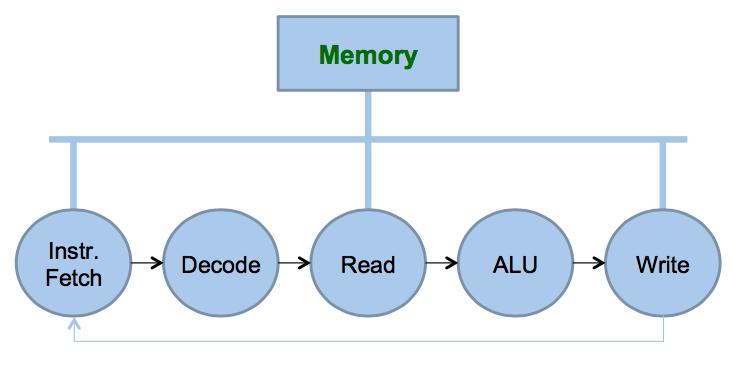
\includegraphics[width=10cm]{images/Chapitre1/Neumann.png}
            \caption{\label{pic_pipeline_simple} Représentation simplifié d'un pipeline de 5 étapes.}
        \end{figure}

        
        \paragraph{Implémentation}
            
            En informatique, la technique de \textit{pipeline} est utilisée pour exploiter le parallélisme d'instructions (ILP) (\autoref{pic_pipeline}). Il est commun de présenter la notion de pipeline avec un pipeline de 5 niveaux:
            
            \begin{itemize}
                \item \textbf{Recherche de l'instruction} ou \textit{fetch}: cette première étape charge l'instruction à exécuter depuis la mémoire principale dans un registre du processeur. Grâce à un compteur interne, le registre \textit{Program Counter}, le processeur connaît l'adresse mémoire de la prochaine instruction à charger. Pour améliorer le temps d'accès aux instructions, le processeur possède un tampon (\textit{instruction buffer}) contenant plusieurs instructions d'avance.
                \item \textbf{Décodage} ou \textit{décode}: une fois que l'instruction est chargée, elle est décodée pour déterminer l'action à exécuter et les données nécessaires.
                \item \textbf{Execution} ou \textit{execute}: en fonction du décodage réalisé, l'instruction est exécutée: utiliser l'ALU pour faire une opération ou calculer une adresse.
                \item \textbf{Accès mémoire} ou \textit{memory}: réalise un accès mémoire (\textit{load} ou \textit{store}) lorsqu'une instruction le nécessite.
                \item \textbf{Ecriture du résultat} ou \textit{write back}: enfin le processeur doit enregistrer le résultat produit par l'étape \textit{execute}. Si c'est un branchement, il modifie le registre \textit{Program Counter} (\textit{branch}). Si c'est une opération arithmétique, il sauvegarde le résultat dans l'adresse destinataire décodé par la deuxième étape.
            \end{itemize}
            
            Le fait de partager l'exécution d'une instruction en sous-étapes permet de commencer l'exécution de la suivante pendant que l'instruction actuelle est encore dans la chaîne d'exécution (voir \autoref{pic_pipeline}). Son utilisation ne réduit pas le temps d'exécution d'une instruction (5 cycles sur la \autoref{pic_pip_no}). Celles-ci doivent tout de même passer une à une par chaque étape de la chaîne. Le \textit{pipeline} permet d'améliorer la cadence d'exécution en maximisant l'utilisation de chaque ressource à un même moment (\autoref{pic_pip_yes}). On peut par exemple commencer à charger la prochaine instruction (étape \textit{fetch}), alors que l'instruction actuelle est en train d'être exécutée (étape \textit{execute}). Sur la \autoref{pic_pip_yes} on assiste à l'exécution de 5 instructions, au premier temps une seule instruction est exécutée, à l'étape $IF$ pour \textit{instruction fetch}. Ensuite, une nouvelle instruction est chargée (opération $IF$) pendant que la première est passée à l'étape suivante (opération $ID$). Ainsi au bout de 5 cycles, chaque étape du pipeline est utilisée (partie en verte). 
            
            
            \begin{figure}
                \begin{subfigure}[]{0.5\linewidth}\centering
                    \vspace{1.6cm}
                    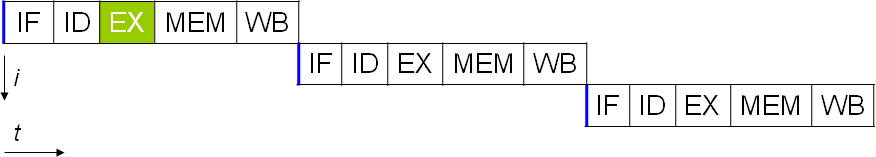
\includegraphics[width=\linewidth]{images/Chapitre1/pipelineNo.png}
                    \caption{Processeur sans pipeline \label{pic_pip_no}}
                \end{subfigure}%
                ~ %space
                \begin{subfigure}[]{0.5\linewidth}\centering
                    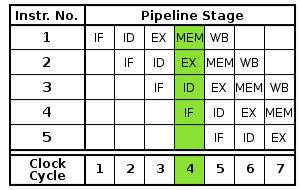
\includegraphics[width=.7\linewidth]{images/Chapitre1/pipelineYes.png}
                    \caption{Processeur avec un pipeline à 5 étages \label{pic_pip_yes}}
                \end{subfigure}
                
                \caption{Pipeline\protect\footnotemark: en séquençant les instructions, le processeur est capable d'exécuter des étapes différentes en parallèle (\textit{IF: instruction fetch, ID: instruction decode, EX: execution, MEM: memory, WB: write back}). Le nombre de cycles nécessaires pour l'exécution de 3 instructions passe alors de 15 à 9 cycles}
                \label{pic_pipeline}
            \end{figure}
            \footnotetext{source - \url{https://fr.wikipedia.org/wiki/Pipeline_(architecture_des_processeurs)}}
            
            
        
        
        \paragraph{Taille du pipeline.}
        
            En 1939 IBM conçoit le premier processeur avec pipeline. Ce n'est qu'en 1989 qu'Intel produira le sien (Intel 80486). Le nombre d'étapes (ou profondeur du pipeline) était de deux à l'origine. Cette taille a augmenté au fil du temps atteignant 31 étapes pour l'architecture du Pentium 4 Prescott d'Intel en 2004. 
        
        \paragraph{Complexité de la gestion du pipeline.}
            
            L'utilisation d'un \textit{pipeline} n'est pas toujours optimale et plusieurs facteurs peuvent affecter sa performance. Le principe du pipeline repose sur le concept de commencer à exécuter des instructions avant que la précédente ne soit terminée. Cela peut être rendu impossible par la dépendance entre deux instructions et par l'utilisation de branchements conditionnels \cite{emma1987characterization}. Lors de l'évaluation d'un tel branchement, le pipeline ne peut pas commencer à exécuter les instructions suivantes sans connaître son résultat. Le processeur doit alors attendre (\textit{stall}) plusieurs cycles avant de continuer. Une optimisation de prédiction de branchement a été implémentée pour éviter ces états de \textit{stall} (voir \autoref{sec:branch_predictor}). De plus, pour permettre la bonne utilisation du pipeline, des mémoires tampons doivent être disposées entre chaque étape pour mémoriser les différents résultats intermédiaires. Lorsque le processeur exécute plusieurs processus, il doit veiller à terminer l'exécution des instructions avant de commencer celles du processus suivant. La complexité de sa gestion le rend vulnérable aux attaques informatiques (voir \autoref{sec:out_of_order}). 
        










    
    
    \subsubsection{Processeur superscalaire} \label{sec:superscalar}
    %%%%%%%%%%%%%%%%%%%%%%
        
        Le pipeline apporte un niveau de parallélisation horizontale. Les processeurs ont reçu une autre amélioration apportant au pipeline une parallélisation verticale. 
        
        \paragraph{Principe}
        
            Un processeur est dit \textit{superscalaire} s'il est capable d'exécuter plus d'une instruction simultanément. Le nombre d'instructions par cycle d'horlge (IPC) peut alors être supérieur à 1. Le principe est d'implémenter un second pipeline (ou plus) capable d'exécuter les instructions telles que sur la \autoref{pic_pip_yes}. Intel proposa son premier processeur superscalaire en 1989 avec le processeur Intel 80486. Il possédait un pipeline à cinq étages proche de celui présenté dans la section précédente. 
            Pour pouvoir l'utiliser, le processeur doit déterminer si deux instructions peuvent être exécutées en parallèle (sans dépendance et utilisant des ressources matérielles différentes). La \autoref{pic_superscalar} montre comment une implémentation superscalaire du pipeline fonctionne. 
            
            \begin{figure}
                \center
                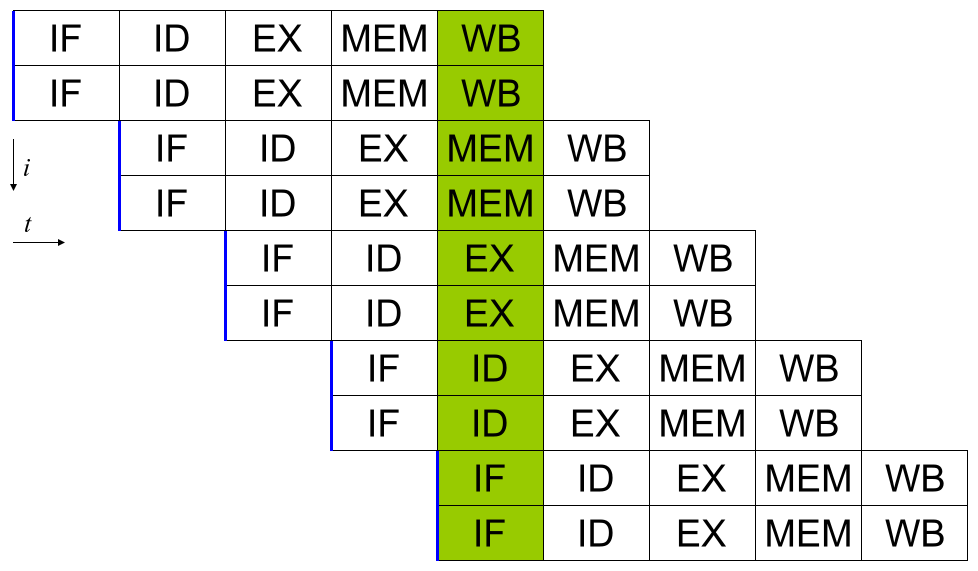
\includegraphics[width=8cm]{images/Chapitre1/superscalar.png}
                \caption[Processeur superscalaire]{Fonctionnement d'un processeur superscalaire possédant deux pipelines.\protect\footnotemark. \label{pic_superscalar} }
            \end{figure}
            \footnotetext{source: \url{https://fr.wikipedia.org/wiki/Processeur_superscalaire}}
        
        
        \paragraph{Implémentation}
        
            Il existe deux façons de transformer un processeur scalaire en superscalaire. La première est de dupliquer matériellement chaque étape pour obtenir deux pipelines distincts (processeurs \textit{superpipeline}). On peut citer le processeur Intel Pentium dont la totalité du pipeline n'est pas dupliquée. Le processeur à une fenêtre de plusieurs instructions prêtes à être exécutées. Seule la phase d'exécution est dupliquée.  Il possédait deux unités d'exécution \textit{u} et \textit{v} qui pouvait exécuter des instructions de types différents (opérations flottantes ou entières) en parallèle. 
            Le deuxième moyen d'implémenter le parallélisme d'instruction d'un processeur superscalaire repose sur le fait qu'une étape peut nécessiter moins d'un demi-cycle d'horloge pour être exécutée. Une étape (ou micro-instruction) du pipeline peut donc s'occuper de deux instructions différentes pendant un cycle d'horloge, en utilisant sa propre horloge interne. Cette méthode a le bénéfice de ne pas avoir a dupliquer le pipeline matériellement. 
            
            Les principales limitations à l'implémentation d'un pipeline sont les dépendances et les conflits. Cela peut être une dépendance entre les données de plusieurs instructions ou un conflit d'accès à une même ressource (ALU, FPU). Le processeur est alors en charge d'orchestrer les différentes instructions pour rendre possible le parallélisme en utilisant des stratégies \textit{d'émission} \cite{johnson1989super} des instructions. Cette stratégie doit veiller à conserver la validité du programme en veillant aux ordres: de lecture des instructions, de leur exécution et de leur actualisation des registres (ou de la mémoire). 
        
        
        \paragraph{Exemple du Pentium 4}\label{sec:alu_pentium}
        
            Pour bien comprendre le déroulement de l'exécution du pipeline d'un processeur superscalaire, nous choisissons de détailler le fonctionnement de processeur Intel Pentium 4 \cite{stallings2003organisation} donc le schéma de la microarchitecture est présenté sur la \autoref{cpu_superscalar_pentium}. Le processeur exécute les \textit{micro-ops} en utilisant un pipeline d'au moins 20 étages en veillant à respecter les dépendances, dont les principales étapes sont décrites ici: 
            
            \begin{enumerate}     
            \item Le processeur lit les instructions (CISC) depuis le cache L2 par groupe de 64 octets dans l'ordre du programme pour profiter de l'effet de localité. Bien que la prédiction de branchement puisse modifier cet ordre. 
            \item Chaque instruction (pouvant être de taille différente) est décodée et traduite en une à quatre instructions RISC de 118 bits (\textit{micro-ops}). 
            \item Ces micro-ops sont ensuite stockés dans un buffer (\textit{Trace Cache}) permettant l'utilisation de l'exécution dans le désordre (voir \autoref{sec:out_of_order}).
            \item Ensuite, le processeur procède au renommage des registres. Il existe 16 registres architecturaux (utilisable par le code) mais 128 registres physiques sont réellement implémentés. Les \textit{micro-ops} peuvent ensuite être stockée dans deux listes d'attente distinctes utilisant une discipline \textit{FIFO}.
            \item L'ordonnanceur choisi ensuite dans les deux files les instructions qui possèdent leurs opérandes et dont l'exécution peut être réalisée. Suivant le type d'instruction, elles sont envoyées (jusqu'à 6 à la fois) vers l'unité d'exécution correspondante (calcul entier ou flottant) en utilisant les différents ports. 
            \end{enumerate}
                 
            
            \begin{figure}
                \center
                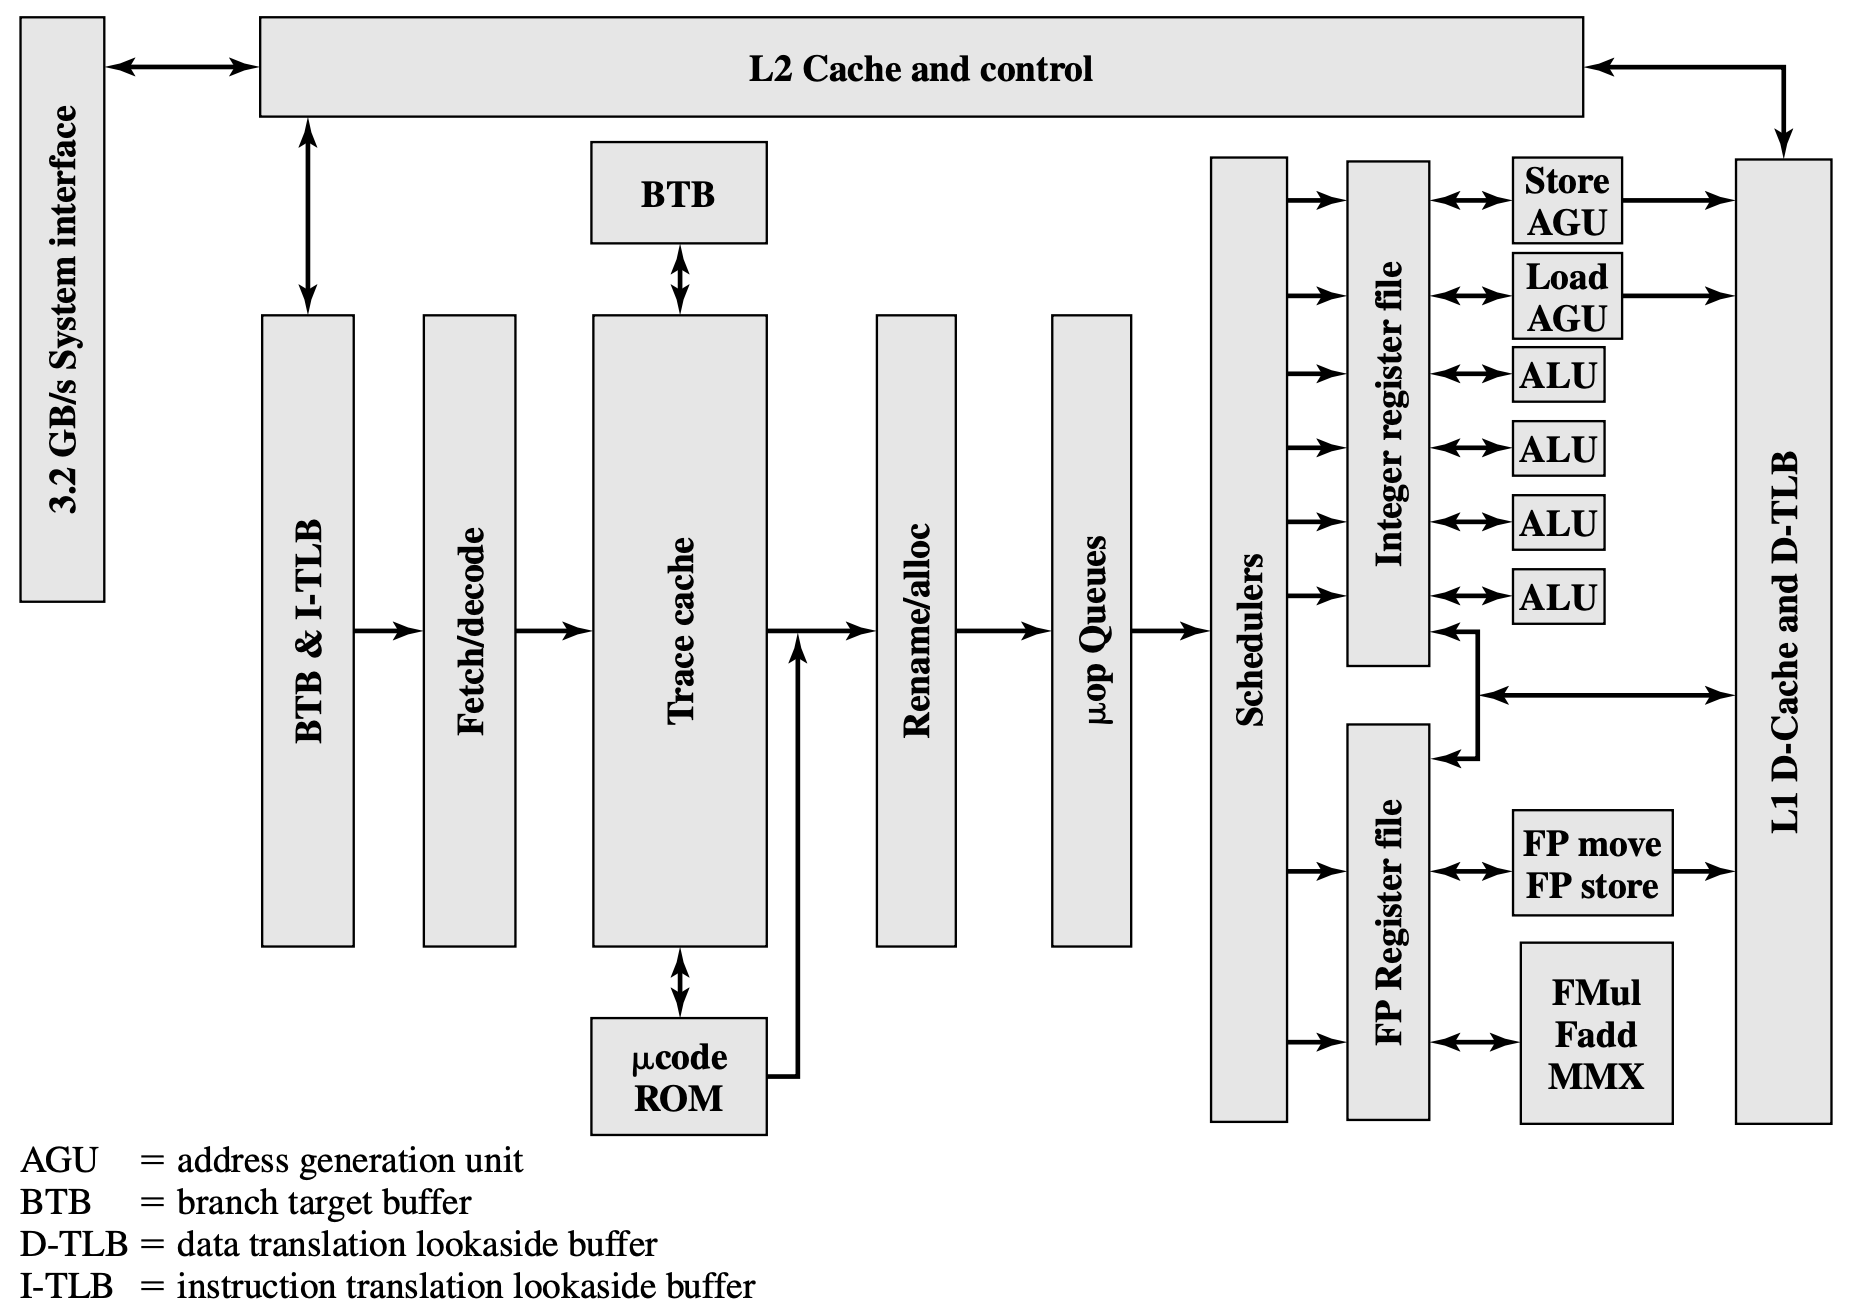
\includegraphics[width=13cm]{images/cpu_superscalar_pentium.png}
                \caption[Diagramme en bloc du Pentium 4]{Diagramme en bloc du Pentium 4 \cite{stallings2003organisation}
                \label{cpu_superscalar_pentium}}
            \end{figure}
            
            
            
            Les architectures actuelles ont beaucoup évolué depuis le premier pentium. Le détail de la microarchitecture Skylake d'Intel peut être consultée sur la \autoref{pic_cpu_skylake_architecture}. L'unité d'exécution peut être utilisée par 8 \textit{ports} différents. Chaque port est relié à des composants différents de l'ALU qui peut exécuter jusqu'à 4 instructions par cycles (ou 2 opérations flottantes).
            
            
            \begin{figure}[hbtp]
                \center
                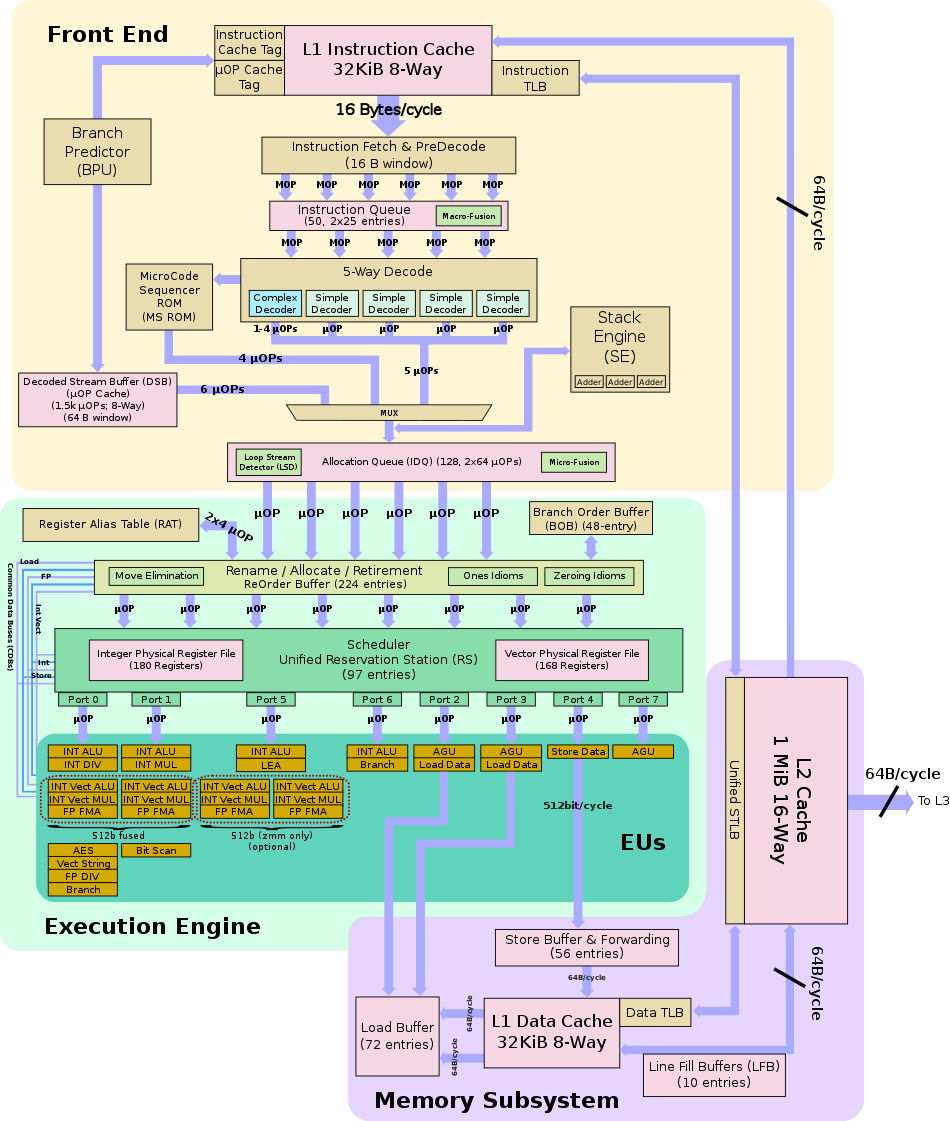
\includegraphics[width=14cm]{images/cpu_skylake_architecture.png}
                \caption{\label{pic_cpu_skylake_architecture}Micro-architecture des processeurs Skylake.}
            \end{figure}
            
            

    
    
    \subsubsection{Processeur multi-coeurs} \label{sec:multicore}
    %%%%%%%%%%%%%%%%%%%%%%
    
           La vitesse de calcul des processeurs est liée à sa fréquence. Cette dernière a largement contribué à l'évolution de leur performance. Cependant, certaines limites physiques empêchent l'augmentation infinie des fréquences (discuté dans la partie \ref{sec:frequency}). Il a donc fallu trouver d'autres moyens d'améliorer la performance des processeurs, sans pouvoir accélérer leur fréquence. L'apparition des processeurs multi-coeurs est une réponse à ce défis. Pour comprendre leur intérêt l'analogie suivante peut être utilisée \cite{tanenbaum2016structured}: la construction d'un processeur avec une fréquence de 1000 GHz est probablement impossible. Par contre, l'utilisation de 1000 processeurs avec une fréquence de 1 Ghz est possible et permet d'obtenir la même performance. Ce gain de performance peut alors être utilisé pour réduire la fréquence des processeurs. En réduisant la fréquence de 30\%, l'énergie nécessaire est réduite de 35\% \cite{mattsson2014haven}. En utilisant deux coeurs à 70\% de la fréquence initiale permet cependant d'obtenir un gain de 140\% de la puissance de calcul totale. C'est ce constat qui motive l'utilisation du parallélisme dans toute l'architecture d'un supercalculateur (voir \autoref{sec:prog_partagee}). Ainsi, avant l'apparition des processeurs multicoeurs, l'utilisation du multitraitement symétrique (SMP) utilisant plusieurs processeurs en parallèle était le principal moyen d'accéder au parallélisme. Cependant, les serveurs devenant toujours plus gros, et avec le désir d'avoir des processeurs plus puissant pour les ordinateurs personnels et les téléphones, les processeurs multi-coeurs ont été inventés.
        
        
        \paragraph{Multi-coeur.}
        
            Le terme de processeur multi-coeur est employé pour désigner tout processeur possédant entre deux et quelques dizaines de coeurs (on parle de processeurs \textit{manycore} au-delà). Les différents coeurs sont disposés sur la même puce d'où l'autre appellation utilisée pour désigner ces processeurs de Chip Multiprocessor (CMP).
            
            Les différents coeurs sont généralement identiques en tout point (processeur homogène) bien qu'ils puissent être différents (processeur hétérogène). Les processeurs homogènes sont plus faciles à utiliser, car tous les coeurs peuvent répondre au même besoin et leur design est plus simple. Les processeurs hétérogènes sont cependant plus performants pour certaines applications. 
            Généralement, chaque coeur du processeur n'est pas relié directement à la mémoire. Un niveau de cache est généralement interposé entre le coeur et la mémoire. La hiérarchie mémoire est présentée dans la \autoref{sec:hierarchie}.
            
            \begin{figure}
                \center
                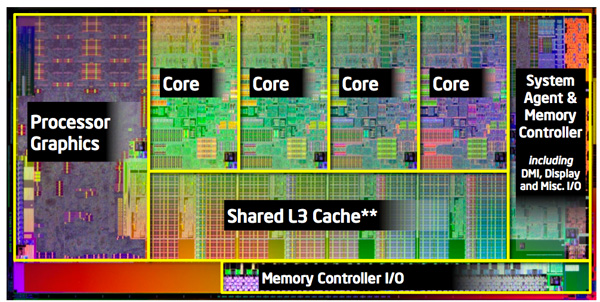
\includegraphics[width=10cm]{images/cpu_multicore.jpg}
                \caption{\label{processeur_archi} Exemple de processeur multi-coeur (Intel Core i7-2600K)  partageant le troisième niveau de cache\protect\footnotemark.}
            \end{figure}
            
            \footnotetext{source: \url{https://www.anandtech.com/show/4083/the-sandy-bridge-review-intel-core-i7-2600k-i5-2500k-core-i3-2100-tested}}
            
            
            
            L'avantage principal de dupliquer un coeur plutôt que de doubler la fréquence d'un seul coeur est la consommation électrique et donc la puissance dégagée par effet Joule. En effet, la puissance dissipée est quadruplée quand la fréquence est doublée alors qu'elle ne fait que doubler lorsque le nombre de coeurs est doublé. On obtient ainsi un processeur utilisant moins d'énergie et nécessitant moins de refroidissement pour une même performance qu'un processeur plus rapide.
            Comme pour le pipeline (voir \autoref{sec:pipeline}), le gain de performance apporté par l'ajout de coeur s'appuie sur l'amélioration du niveau de parallélisme d'instructions (Instruction Level Parallélisme (ILP)).
            
            
            La difficulté d'utilisation de processeurs multi-coeurs vient des programmes qui ne sont pas capables par nature d'utiliser ce niveau de parallélisme. Ils doivent donc être programmés pour pouvoir en profiter. Cette tâche, quoique difficile à ses débuts, est aujourd'hui facilitée par l'utilisation de librairies prévues telles que \textit{Pthread} ou \textit{OpenMP}. 
            
            Les coeurs partagent des niveaux communs de cache (généralement le dernier), la bonne programmation des applications et l'implémentation d'une microarchitecture efficace sont alors des facteurs déterminants de la performance obtenue:
            \begin{itemize}
                \item Pour maximiser l'utilisation des caches, il est primordial de prévoir leurs partages entre les différents coeurs pour minimiser les conflits. Des méthodes de placements plus ou moins efficaces peuvent alors être utilisées \cite{mazouz2011performance}: laisser le système d'exploitation s'en occuper peut donner des performances très variables entre deux exécutions identiques, alors que le placement manuel permet d'obtenir les meilleurs résultats. 
                \item Le choix du réseau utilisé par les coeurs est alors important pour la performance des codes et repose principalement sur quatre paramètres \cite{peh2009chip} : la topologie, les algorithmes de routages, le protocole de contrôle de flux et le routage de la microarchitecture. La topologie indique comment les coeurs sont connectés et quels sont les chemins empruntables par un message pour rejoindre sa destination. Ce choix est réalisé par l'algorithme de routage. Le contrôle de flux s'occupe de l'envoi des messages (ordre et date d'envoi) qui est ensuite réalisé par la microarchitecture. Les choix réalisés pour ces quatre paramètres ont un impact sur la performance du processeur (latence, bande passante) et sur son prix. 
            
            \end{itemize}
            
            Le nombre de coeurs par processeur a beaucoup évolué durant les quinze dernières années. Si les premiers processeurs multi-coeurs n'en possédaient que deux, il n'est pas rare que les supercalculateurs utilisent des processeurs avec plus de vingt coeurs. Intel à même annoncé en 2019 un nouveau processeur doté de 56 coeurs \footnote{\url{https://ark.intel.com/content/www/us/en/ark/products/194146/intel-xeon-platinum-9282-processor-77m-cache-2-60-ghz.html}}. Cependant, l'ajout de coeurs supplémentaires n'est pas forcément bénéfique pour les applications à cause de la vitesse des mémoires qui peinent à évoluer au même rythme. Ce constat est discuté dans la \autoref{sec:memory}.
        \section{Hiérarchie mémoire} \label{sec:hierarchie}
%%%%%%%%%%%%%%%%%%%%%%%%%%%%%%%%%%%%%%%%%%%%%%%%%%%%%%%%%%%%%%%%%%%

Dans la partie précédente sont présentées les principales améliorations dont la microarchitecture a pu  bénéficier. Cette partie s'intéressait principalement à l'exécution des instructions. Pour être exécutées, ces instructions ont besoin de données stockées en mémoire. La performance totale du processeur dépend donc à la fois de la vitesse d'exécution des instructions, mais aussi de la capacité de la microarchitecture à transférer les données nécessaires au processeur. Cette section s'intéresse donc plus précisément à la partie mémoire:
\begin{itemize}
    \item  La \autoref{sec:memory} présente la différence d'évolution entre les processeurs et la mémoire. 
    \item Cette introduction permet de motiver la nécessité de construire une hiérarchie mémoire présentée dans la \autoref{sec:hierarchie_true}. 
    \item Enfin, la \autoref{sec:cache} présente plus précisément les mémoires caches.
\end{itemize}

%%%%%%%%%%%%%%%%%%%%%%%%%%%%%%%%%%%%%%%%%%%%%%%%%%%%%%%%%%%%%%%%%%%
\subsection{Mémoire principale} \label{sec:memory}
%%%%%%%%%%%%%%%%%%%%%%%%%%%%%%%%%%%%%%%%%%%%%%%%%%%%%%%%%%%%%%%%%%%
%%%%%%%%%%%%%%%%%%%%%%%%%%%%%%%%%%%%%%%%%%%%%%%%%%%%%%%%%%%%%%%%%%%

Pour leur exécution, les processeurs doivent accéder aux instructions et aux données stockées en mémoire. Celles-ci sont principalement construites à partir de mémoire RAM (voir \autoref{sec:ram}). Bien que celles-ci est profité de la miniaturisation des transistors les composant (voir \autoref{sec:moore}), l'industrie a constaté depuis plusieurs années un écart de performance entre le système mémoire et la puissance de calcul du processeur.


    \subsubsection{Performance de la mémoire et des processeurs}
    %%%%%%%%%%%%%
    
        Grâce aux nombreuses améliorations apportées aux processeurs (voir \autoref{sec:micro}), l'écart entre leur performance et celle des mémoires s'est creusé au fil des années (voir \autoref{pic:cpuvsmemory}).  Ce graphique montre que l'écart de performance entre les deux s’agrandit exponentiellement au fil des ans (utilisation d'une échelle logarithmique en ordonnée) :
       \begin{itemize}                 
            \item La performance calculatoire des processeurs (\gls{FLOP} exécutable par cycle) a \textbf{augmenté de 50\%} en moyenne par an.
            \item La bande passante entre le processeur et la mémoire a augmenté de 23\% par an                 
            \item La latence des requêtes mémoires a \textbf{diminué de 4\% } par an                 
            \item La bande passante sur le réseau a \textbf{augmenté de 20\%} par an             
        \end{itemize}
        Ainsi l’augmentation du nombre de coeurs, dont la performance augmente (fréquence, pipeline, opérations vectorielles), se partageant le bus mémoire dont les performances évoluent lentement, implique une baisse de bande passante disponible par coeur (voir \autoref{pic_cpu_bw_per_core}). 
         
        \begin{figure}[ht!]
            \centering
            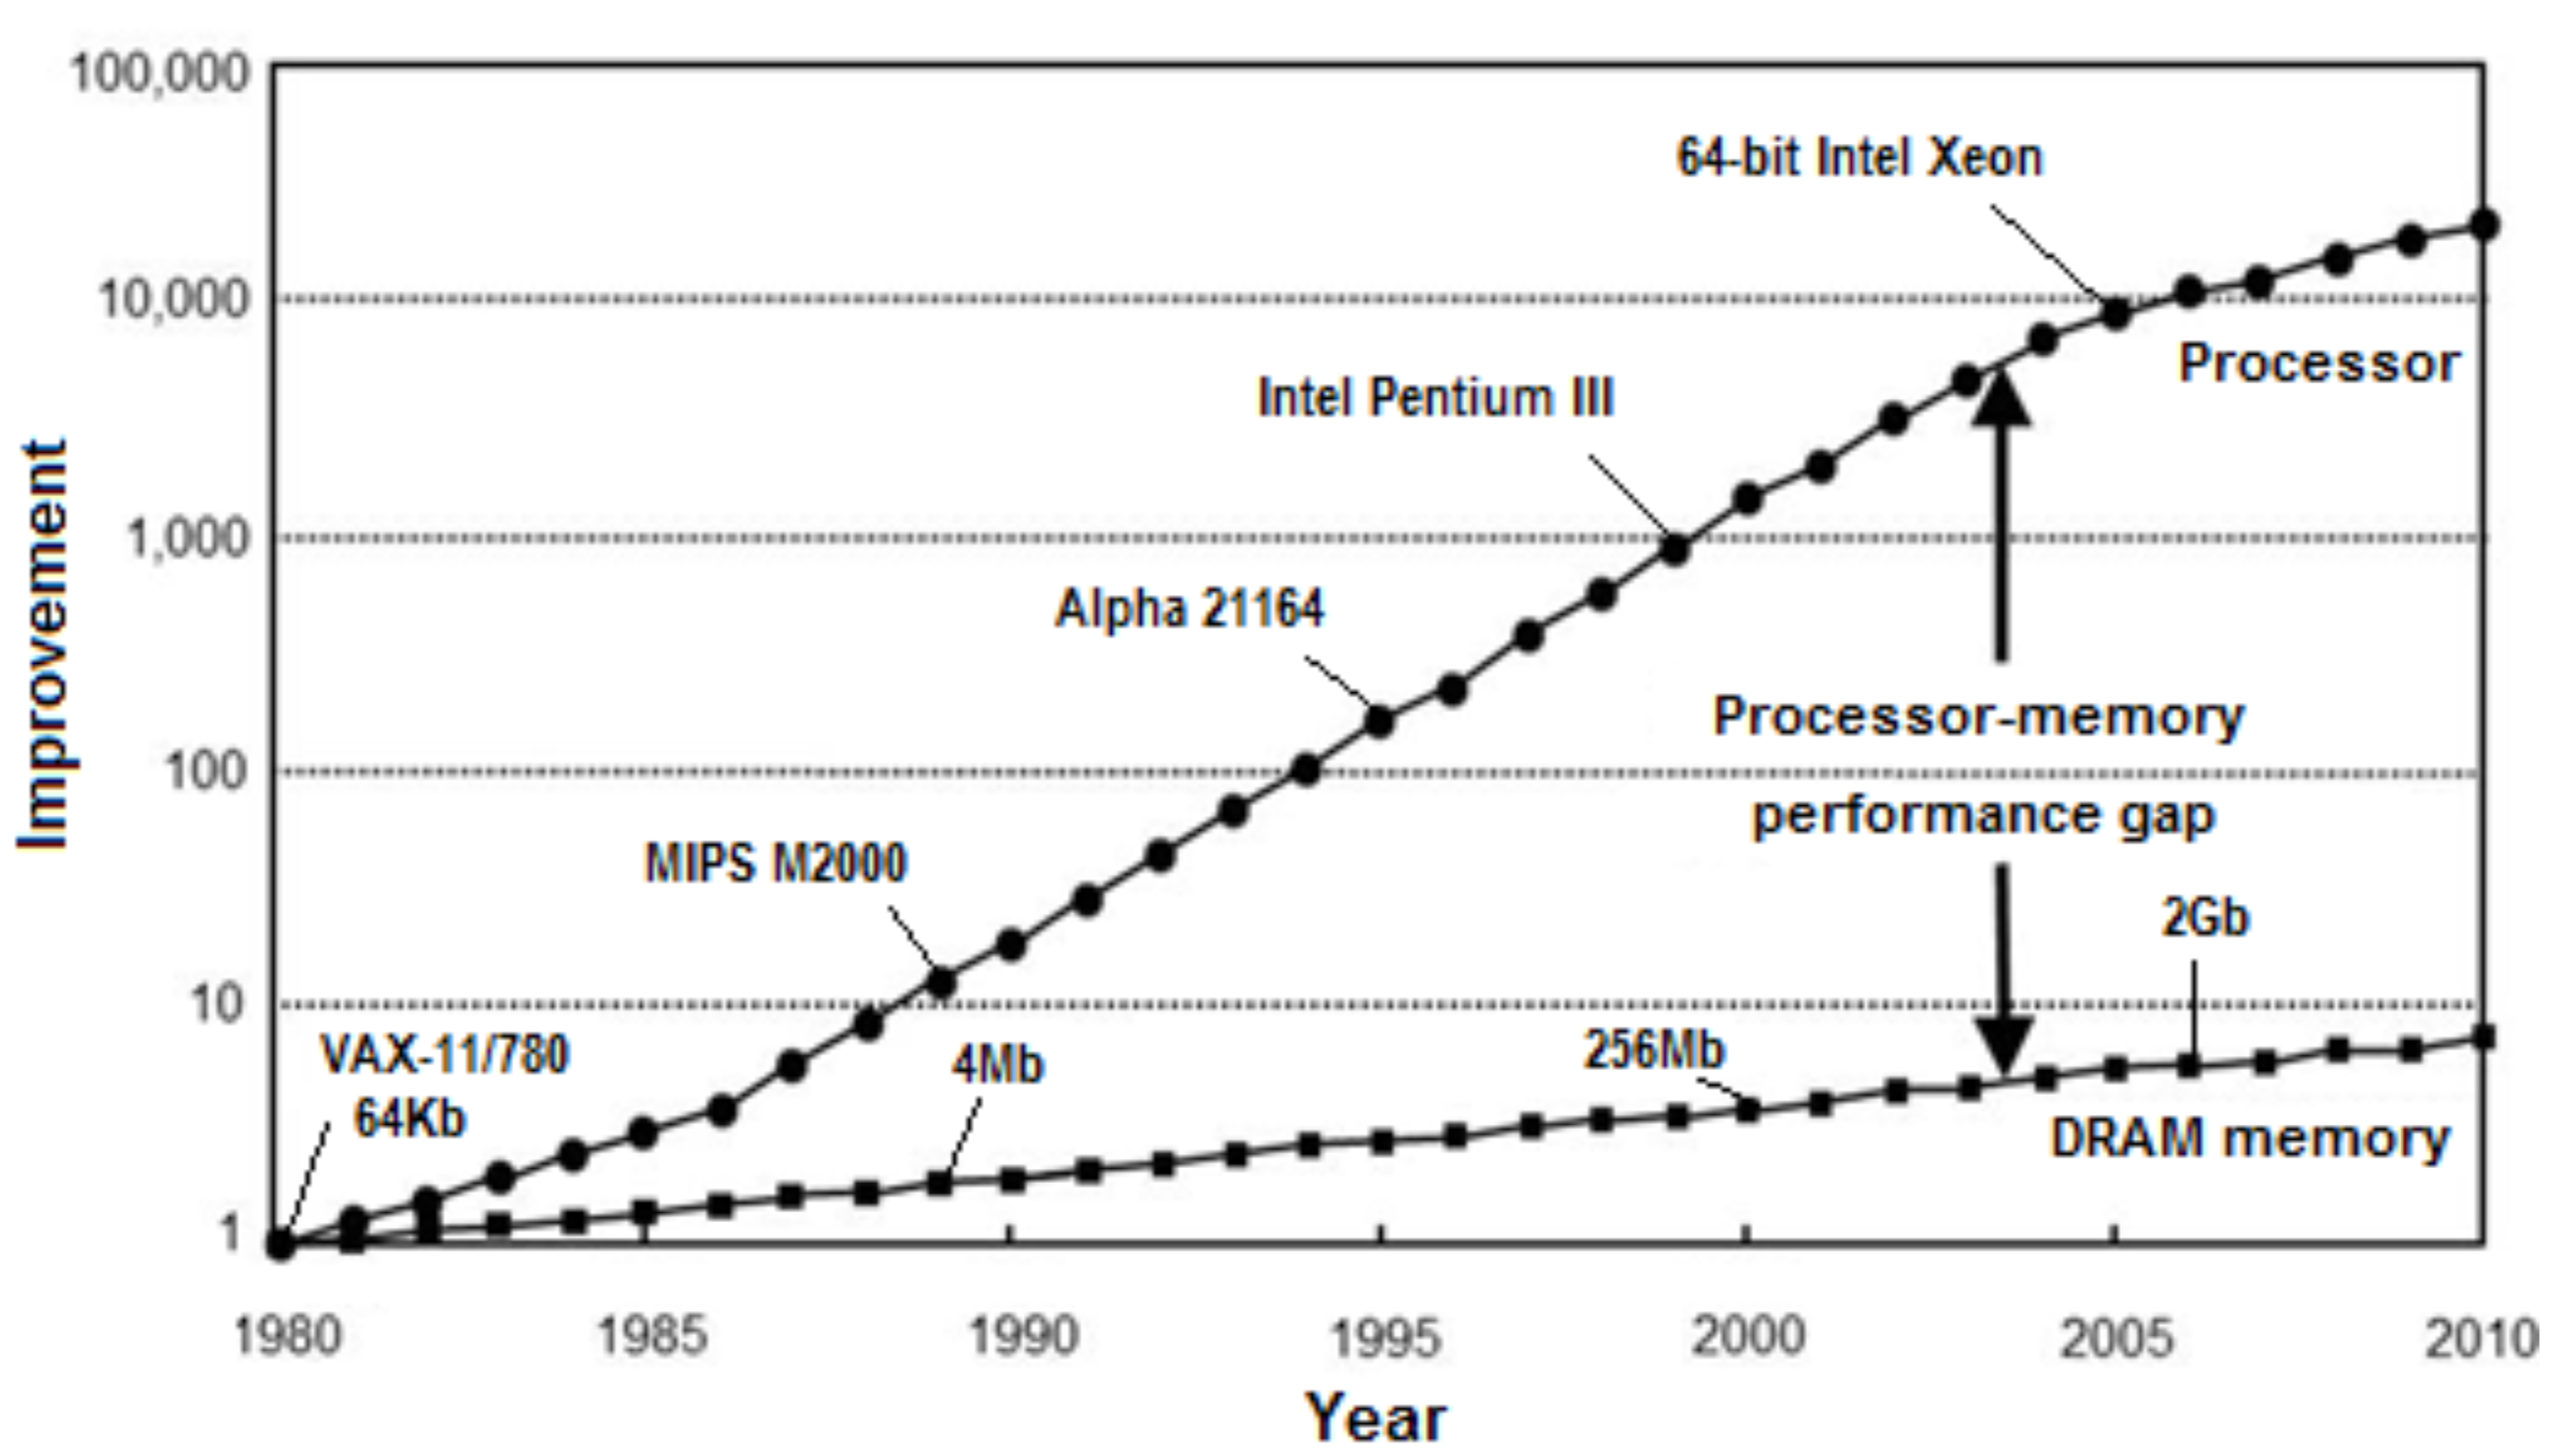
\includegraphics[width=14cm]{images/cpu_cpu_vs_memory.png}            \caption{\label{pic:cpuvsmemory} Progression de la performance des processeurs et des mémoires. La performance de plusieurs générations de processeurs a été mesurée à l'aide du benchmark SPECint \cite{Efnusheva2017ASO}. La performance des mémoires est la mesure des latences d’accès mémoire (CAS et RAS) des mémoires DRAM.}

            \vspace*{\floatsep}% https://tex.stackexchange.com/q/26521/5764

            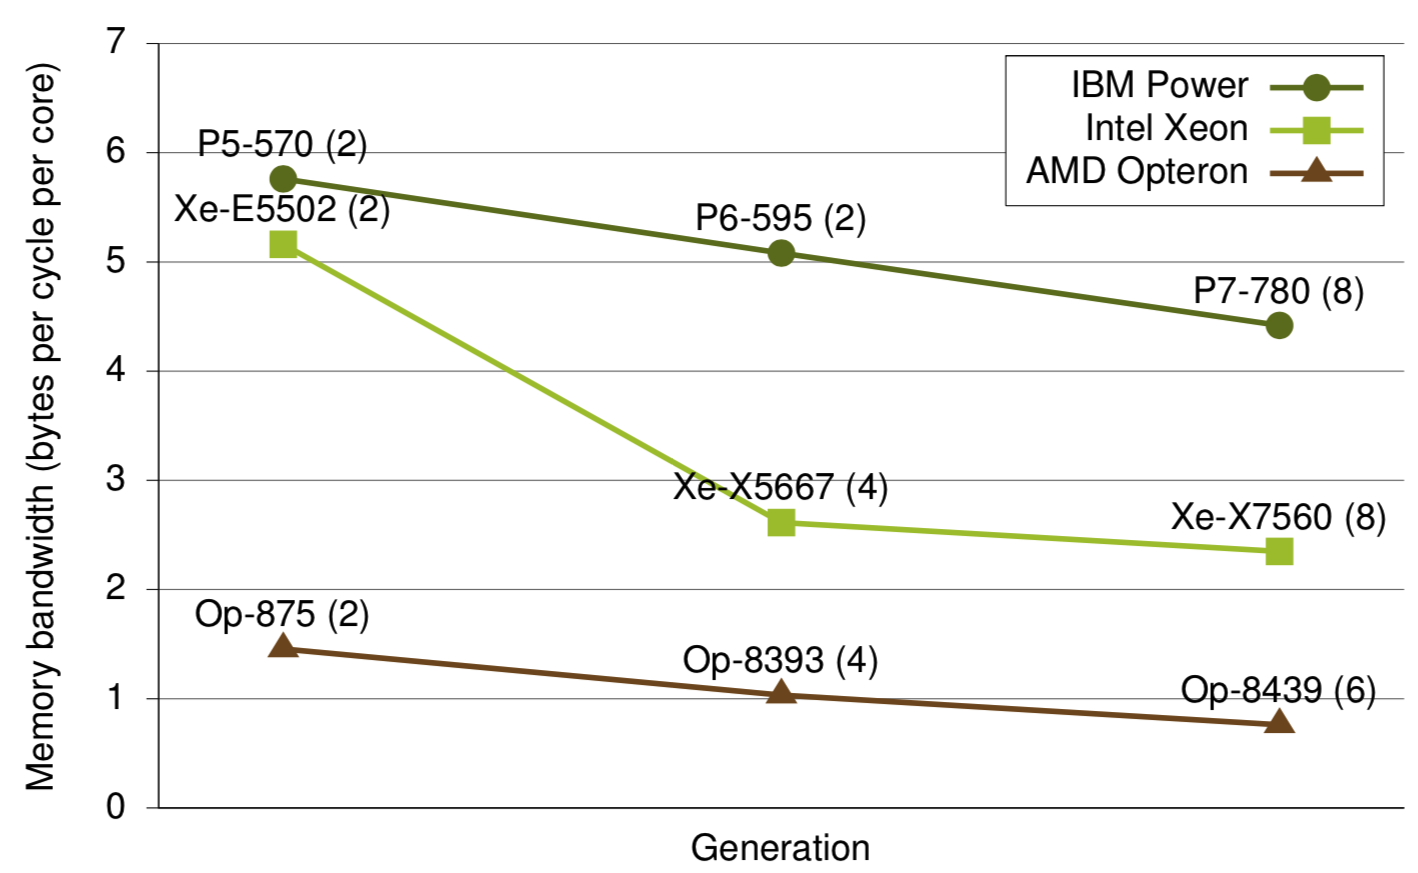
\includegraphics[width=14cm]{images/cpu_bw_per_core.png}
            \caption{Évolution de la bande passante bande passante par cycle d'horloge par coeur. L'évolution du nombre de coeurs et de leur fréquence n'est pas compensée par l'évolution de la performance du système mémoire.
            \label{pic_cpu_bw_per_core}}
        \end{figure}
        

    \subsubsection{Le mur de la mémoire}\label{sec:memory_wall_gap}
    
        L'écart croissant entre les performances de la mémoire et des processeurs est souvent appelé \textit{mur de la mémoire} (\textit{memory wall}). Cette expression été déjà utilisée en 1995 \cite{Wulf1995} dans le papier \textit{Hitting the Memory Wall: Implications of the Obvious}. Plusieurs raisons peuvent expliquer cet écart de performance.
    
        Une première raison pouvant expliquer l'apparition de cet écart de performance est l'économie du marché des mémoires. Le prix par gigaoctet diminue avec la densité des mémoires. Les fabricants d'ordinateurs et de téléphones souhaitent avoir des mémoires de plus grande capacité dans des espaces restreints avec des contraintes énergétiques. La SRAM, moins dense et plus consommatrice est ainsi passée en second plan. Le gain de transistors assuré par la loi de Moore a été utilisé pour construire des mémoires plus denses et donc de plus grande capacité. Cependant, l’industrie des microprocesseurs a profité de ces transistors pour construire des processeurs plus performants tandis que l’industrie des mémoires en a profité pour créer des mémoires de plus grande capacité. 
            
        La seconde raison est technologique. Les différentes évolutions de ces deux technologies mémoire sont résumées dans le \autoref{tab_ddr}.  La mémoire DRAM à vu ses performances évoluer d'un facteur 10 depuis les premières versions de \textit{SDRAM} dans les années 90. Le passage de la SDRAM à la \textit{Double Data Rate} (DRAM) permet d'envoyer deux données par signal d'horloge. Les principales évolutions des performances de ces technologies sont résumées dans le \autoref{tab_ddr}. 
        Aussi, l’architecture Von Neumann (voir \autoref{sec:von}) implémente une microarchitecture qui sépare la partie exécution de la partie mémoire. Le processeur a besoin des instructions et des données stockées dans la mémoire ce qui implique de nombreuses communications entre ces deux parties. Le bus mémoire devient un \gls{bottleneck} pour les performances. Ce goulot a ainsi été nommé d'après l'architecte: le \textit{bottleneck Von Neumann}.
            
             
            \begin{table}[]
            \centering
            \resizebox{\textwidth}{!}{%
            \begin{tabular}{@{}|l|c|c|c|c|c|@{}}
            \toprule
            \rowcolor[HTML]{EFEFEF} 
            \textbf{DDR Standard} & \multicolumn{1}{l|}{\cellcolor[HTML]{EFEFEF}\textbf{Débit (MT/s)}}     & \multicolumn{1}{l|}{\cellcolor[HTML]{EFEFEF}\textbf{Densité (MiB)}} & \multicolumn{1}{l|}{\cellcolor[HTML]{EFEFEF}\textbf{Bande passante (GB/s)}} & \multicolumn{1}{l|}{\cellcolor[HTML]{EFEFEF}\textbf{Latence (ns)}}           & \multicolumn{1}{l|}{\cellcolor[HTML]{EFEFEF}\textbf{Tension (V)}} \\ \midrule
            SDRAM    &      100-166         & 1          & 0.8-1.3        & 90-75            & 3.3       \\ \midrule
            DDR      &      133-200         & 128         & 1-3.1        & 36-30            & 2.5       \\ \midrule
            DDR2     &      400-1066        & 256         & 3.2-8.3        & 37.5-14.06       & 1.8       \\ \midrule
            DDR3     &      1066-3300       & 1024       & 8.3-25.8       & 19.69-11.82      & 1.5       \\ \midrule
            DDR4     &      1600-4800       & 4096       & 12.5-37.5        & 19.38-9.38       & 1.2       \\ \bottomrule
            \end{tabular}%
            }
            \caption[Évolution des technologies de mémoire DRAM]{Les évolutions des technologies mémoire DDR ont permis d'améliorer les vitesses de transferts d'un facteur dix en divisant par trois leur consommation électrique\protect\footnotemark. Pour chaque standard DDR, les débits et la latence sont donnés pour deux fréquences différentes. La latence mesure le temps nécessaire pour transférer  8 mots (soit une ligne de cache). Cette mesure est plus précise, car les versions les plus récentes de DDR lisent plusieurs mots à la fois dans une mémoire tampon, et profite donc de la localité spatiale.}
            \label{tab_ddr}
            \end{table}
            \footnotetext{source: \url{https://www.transcend-info.com/Support/FAQ-296}, \url{https://promotions.newegg.com/crucial/15-2725/index.html?icid=318028}, \url{https://en.wikipedia.org/wiki/CAS_latency} \url{https://www.crucial.com/usa/en/memory-performance-speed-latency}}
        
            
        
        
    % SOLUTION


    \subsubsection{Latence mémoire}
    
        La latence mémoire représente le temps écoulé entre l’initiation d’un transfert par le contrôleur mémoire du processeur et l'arrivée de la donnée sur le processeur. Afin de réduire ce temps, les architectures ont reçues plusieurs améliorations matérielles et logicielles afin de \textit{tolérer} ou \textit{réduire} les latences mémoires \cite{Efnusheva2017ASO}:
        \begin{itemize}
            \item \textbf{Tolérer} les latences \cite{Bakshi2000} consiste à permettre au processeur de continuer d’exécuter des instructions durant l'attente du transfert d'une donnée. Les processeurs ont reçu plusieurs améliorations matérielles permettant de tolérer l'absence d'une donnée: l’exécution dans le désordre (\autoref{sec:out_of_order}) ou la prédiction de branchement (\autoref{sec:branch_predictor}).
            
            \item \textbf{Réduire} la latence mémoire peut être réalisé de manière logicielle ou matérielle grâce aux techniques de prélecture mémoire (\textit{memory prefteching}) \cite{baer1991effective, mowry1991tolerating}. Ces techniques ont pour objectif de prédire les futurs accès mémoire afin de réduire ou supprimer la latence lors d'un accès mémoire. La prélecture peut être réalisée par le système d'exploitation ou par le compilateur en se basant sur des motifs d'accès pour anticiper les prochains appels mémoires. Elle peut aussi être implémentée manuellement dans l'application en utilisant des instructions spécifiques ou en anticipant les accès. 
        \end{itemize}
        
        %Si les latences peuvent être réduites ou tolérer, la bande passante du bus mémoire contraint elle aussi la performance des applications. La principale réponse à ce challenge est l’implémentation d’une hiérarchie de mémoire plus ou moins rapide en fonction de leur proximité avec le processeur. 
       
        
   
\subsection{La hiérarchie mémoire}\label{sec:hierarchie_true}
%%%%%%%%%%%%%%%%%%%%%%%%%%%%%%%


    \subsubsection{Compromis entre coût, performance et capacité } 
    %%%%%%%%%%%%%%%%%%%%%%%%%%%%%%%%%%%%%%%%%%%%%%%%%%%%%%%%%%%%%%%%%%%
        
        La réponse naïve au problème du \textit{memory wall} est de construire de grandes mémoires à partir de SRAM, très performantes et qui consomment peu d'énergie. Cependant, des contraintes économiques et techniques sont à prendre en compte et rendent impossible cette solution. La mémoire SRAM est très chère à produire et nécessite l'utilisation de six transistors pour fonctionner, empêchant la construction de modules denses. Dans le tableau \ref{pic_cpu_memory_comparison}, on remarque que trois caractéristiques d'une mémoire sont liées:
        \begin{enumerate}
            \item Plus sa latence d'accès est rapide, plus son prix est élevé,
            \item Plus sa capacité mémoire est élevée, plus son prix par bit est réduit.
            \item Plus sa capacité est élevée, plus sa latence d'accès est lente.
        \end{enumerate}
        L'objectif des constructeurs d'ordinateur est de proposer une mémoire de grande capacité, très rapide à un prix le plus faible possible, ce qui n'est malheureusement le cas d'aucune des technologies existantes. Pour atteindre cet objectif, la solution imaginée par les architectes est l'utilisation de différents tailles et types de mémoires constituant une \textit{hiérarchie de mémoires}.
        
        
        \begin{figure}
            \center
            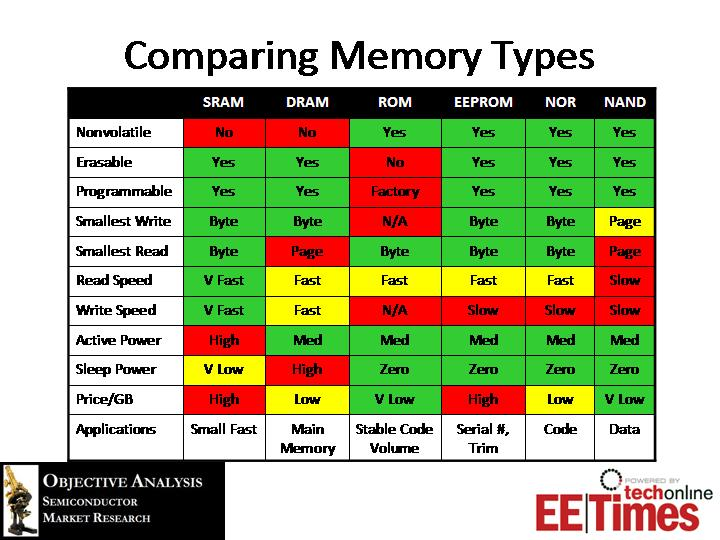
\includegraphics[width=10cm]{images/cpu_memory_comparison.jpg}
            \caption{\label{pic_cpu_memory_comparison} Comparaison des caractéristiques de différents types de mémoires.}
        \end{figure}
        
        
    \subsubsection{Description d'une hiérarchie mémoire} 
    %%%%%%%%%%%%%%%%%%%%%%%%%%%%%%%%%%%%%%%%%%%%%%%%%%%%%%%%%%%%%%%%%%%
    
        
        La hiérarchie mémoire est la réponse d'un compromis entre le coût, la performance et la capacité de stockage pour la construction de la mémoire d'un processeur. Comme aucune des mémoires ne répond à ces trois facteurs à la fois, la solution est de ne pas se restreindre à  une seule technologie et d'utiliser des modules de taille différente (voir \autoref{fig:edl_memory_pyramide2}). Le compromis réalisé par la hiérarchie mémoire permet ainsi de: réduire le coût par bit stocké, augmenter la capacité de la mémoire et améliorer le temps d'accès aux données. 
        
        \begin{figure}
            \center
            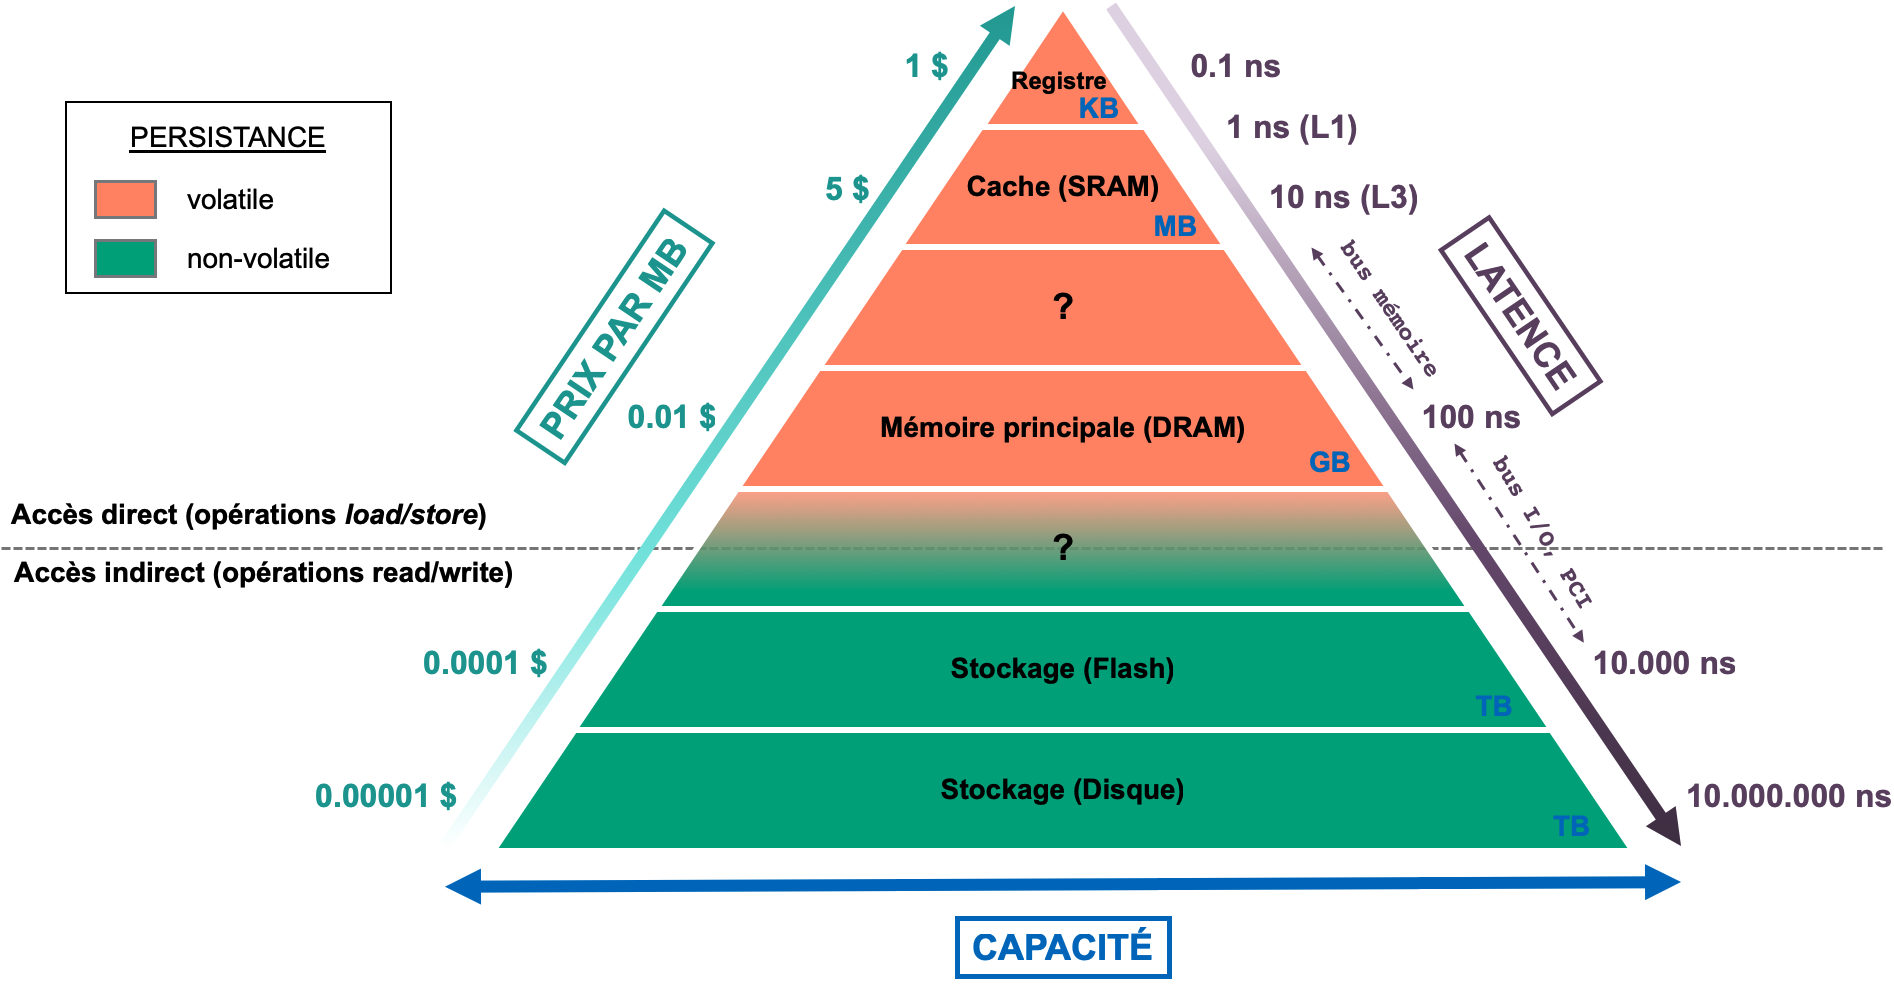
\includegraphics[width=17cm]{images/edl_memory_pyramide.png}
            \caption{\label{fig:edl_memory_pyramide2} Hiérarchisation des différents types de mémoire en fonction du coût, de la latence et de la capacité de stockage habituellement utilisés dans les architectures modernes. Les écarts de performance relevés dans la hiérarchie mémoire sont modélisés par un '?'.}
        \end{figure}
        
        La solution est de placer au plus proche du processeur des mémoires très rapides pouvant répondre instantanément aux accès mémoire. Au plus on s'éloigne des unités de calcul, au plus la latence d'accès aux modules mémoires augmente, mais au plus leur prix diminue rendant possible l'utilisation de module de plus grande capacité. Lorsque le processeur souhaite accéder à une donnée, il vérifie qu'elle se trouve dans son premier niveau de mémoire et, si ce n'est pas le cas, remonte la hiérarchie jusqu'à la trouver. La performance des applications varie fortement si les données nécessaires sont présentes ou non dans les mémoires proches du processeur. L'apport d'un gain de performance de la hiérarchie réside dans le fait que la donnée accédée doit se trouver le plus souvent possible dans les zones mémoires les plus proches du processeur. La \autoref{fig:edl_memory_pyramide2} présente les principaux modules d'une hiérarchie mémoire d'un processeur moderne:
        \begin{enumerate}
            
            \item \textbf{Les registres}: ils sont situés au plus proche des unités de calculs. Pour permettre un accès rapide, inférieurs à 1 cycle, les registres sont réalisés en SRAM. On compte une centaine de registres sur les processeurs récents. Leur taille est variable en fonction des instructions exécutables par les unités logiques arithmétiques. Par exemple, un processeur pouvant exécuter des instructions vectorielles AVX-512, possède des registres de 512 bits (registre \textit{ZMM}). Il existe différents types de registres, certains sont utilisés pour stocker des données et des résultats intermédiaires, tandis que d'autres ont une signification précise. Le registre de pointeurs de piles stocke l'adresse de la première adresse mémoire responsable de l'instruction actuellement exécutée et permet de réaliser des appels et des retours de fonctions. Les registres des drapeaux (Flag Register) stockent des informations nécessaires à l'exécution d'instructions. Par exemple, lorsqu'une retenue est générée par un calcul, ou qu'un branchement conditionnel a été évalué à vrai. Les processeurs récents dupliquent certains registres pour pouvoir utiliser des techniques de renommage \cite{moudgill1993register} et d'exécution spéculative \cite{chou2004efficient}.
        
            \item \textbf{Les caches} ou \textit{antémémoire} sont des modules de mémoire généralement en SRAM à très faible latence d'accès (quelques  cycles). Ces mémoires étant très chères, elles ne peuvent pas être construites en grande quantité. La performance d'une application dépendra fortement de la présence ou non des données nécessaires dans ces mémoires. Ce principe est connu sous le nom de concept de \textit{localité}, présenté dans la \autoref{sec:locality}. Les caches sont présentés plus précisément dans la \autoref{sec:cache}.
            
            \item \textbf{La mémoire} ou mémoire principale, stocke les instructions du programme ainsi que les données nécessaires à leur exécution. Pour des grands jeux de données dépassant la taille de la mémoire, cette dernière agit comme un cache entre le processeur et les modules de stockage.
            
            \item \textbf{Le stockage} est le premier étage de la hiérarchie à utiliser une mémoire non volatile. Ces modules peuvent contenir des téraoctets de données, mais dont les temps d'accès sont extrêmement longs par rapport aux mémoires mentionnées ci-dessus. Leur principal avantage est leur prix.
            
            \item \textbf{La mémoire auxiliaire} est aussi non volatile avec un coût bien plus faible que pour les mémoires de stockage. Sa capacité à stocker les données pendant plusieurs années est utilisée pour stocker et archiver des données de nécessitant pas d'accès immédiat. Les supports sont magnétiques (disques et bandes) ou optiques.
        
        \end{enumerate}
        
        \paragraph{Communication entre les différents niveaux}
        %%%%%%%%%%%%%%%%%%%
            
            Pour communiquer entre les différents niveaux de la hiérarchie, les données sont transmises par bloc de données de tailles différentes (voir \autoref{pic_cpu_memory_hierarchy}). L'avantage de transférer les données par bloc et non une par une est d'améliorer la performance des codes en tirant parti du principe de localité spatiale (voir \autoref{sec:locality}).
            Pour accéder à un mot, le processeur a besoin que celle-ci se trouve dans le niveau de cache L1. Lorsqu'elle s’y trouve, le processeur peut charger un mot directement dans ces registres pour y effectuer les opérations nécessaires. C'est la granularité de transfert la plus petite dans une microarchitecture. Entre les différents niveaux de caches et entre le cache et la mémoire les données sont transférées par blocs appelés \textit{lignes de cache} ou ligne de cache. La ligne de cache contient une copie des données de la mémoire, un tag contenant des informations sur l'adresse mémoire du bloc de données et un \textit{flag} contenant des informations sur la validité de la ligne (voir \autoref{pic:cacheline}). La taille d'une ligne de cache peut varier d'une architecture à l'autre, mais il est courant d'utiliser des tailles de 32, 64 ou 128 octets. Une ligne de cache d'un processeur Intel récent mesure 64 octets. Elle contient ainsi 8 éléments en double précision. Enfin, entre le stockage et la mémoire, les blocs de données transférés sont de la taille d'une page (voir \autoref{sec:page}) qui mesure généralement entre 4 KiB et 2 MiB.
            
            
            
            \begin{figure}
                \center
                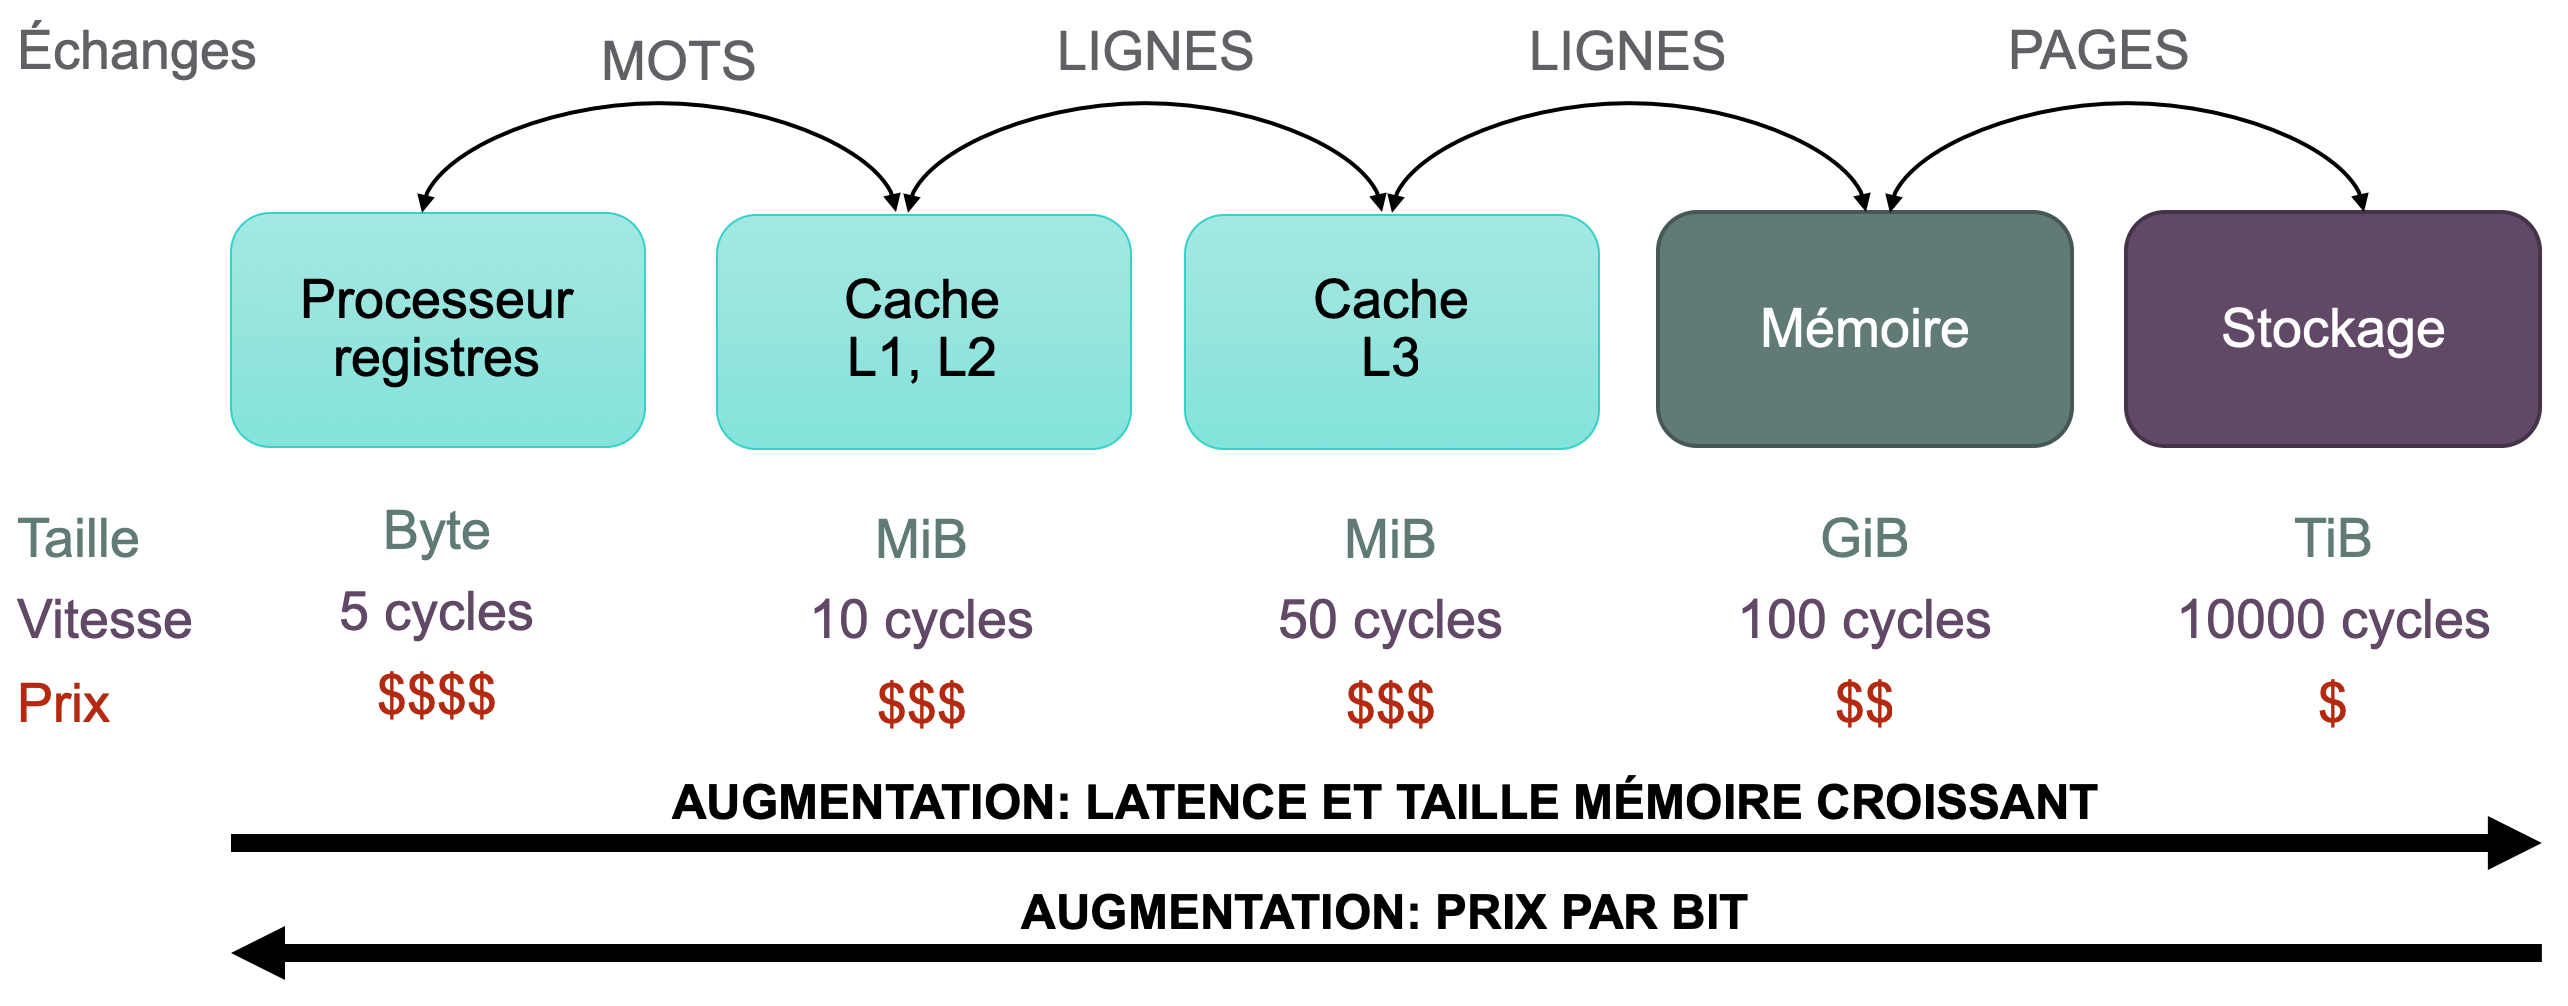
\includegraphics[width=14cm]{images/cpu_memory_hierarchy.png}
                \caption{\label{pic_cpu_memory_hierarchy} Hiérarchie mémoire}
            \end{figure}
            
            \begin{figure}
                \center
                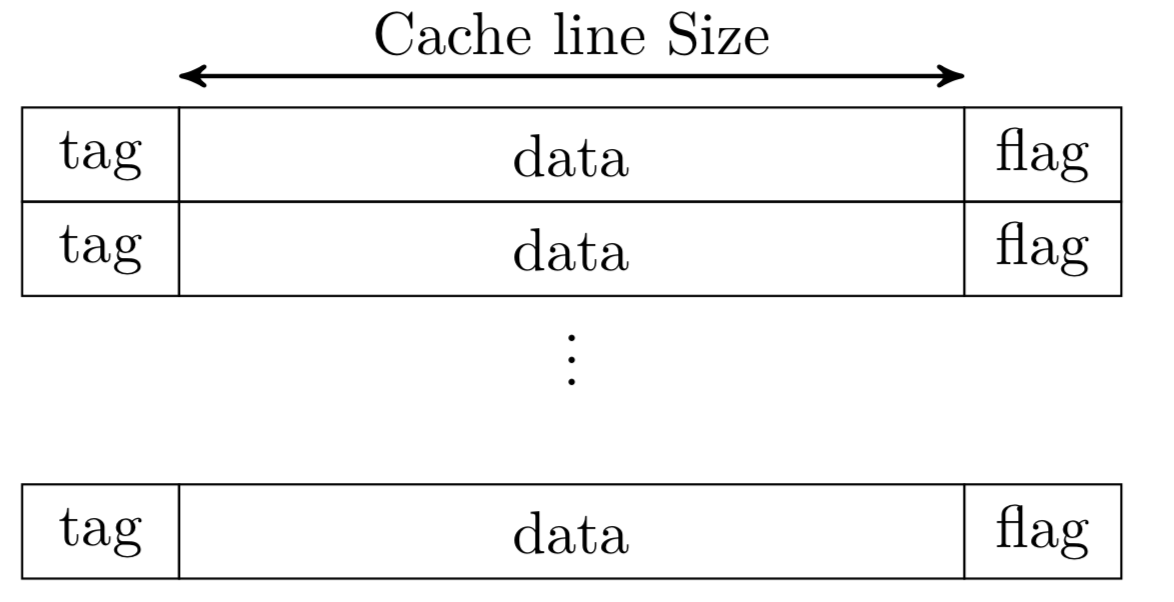
\includegraphics[width=8cm]{images/cacheline_def.png}
                \caption{\label{pic:cacheline} Représentation d'une ligne de cache.}
            \end{figure}
        
        
        %%%%%%%%%%%%%%%%%%%%%%%%%%%%%%%

    
    \subsubsection{Localité}\label{sec:locality}
    

        Mal utilisée, la hiérarchie mémoire n'apporte aucun gain de performance. Son efficacité réside dans la présence des données utilisées dans les niveaux de caches les plus proches de la mémoire. Afin d'améliorer la performance des applications, il est nécessaire de profiter de la localité des données. Le principe de localité exprime la faculté d'un programme à utiliser des données présente dans les premiers niveaux de cache. Elle peut être de deux types:
        \begin{itemize}
            \item \textbf{La localité spatiale} s'appuie sur l'utilisation de données dont les adresses sont consécutives en mémoire (accès encadré en vert sur la \autoref{pic_cpu_locality}). En effet, la taille d'un bloc de données transféré (une ligne de cache), mesure plusieurs octets et contient plusieurs éléments. Un programme utilisant des données consécutives en mémoire, aura la chance de trouver la donnée suivante déjà chargée dans le cache.  Par exemple, les instructions d'un programme se suivent en mémoire et sont accédées consécutivement.
            \item \textbf{La localité temporelle} exprime la réutilisation d'une donnée dans un futur proche, augmentant la probabilité qu'elle soit toujours dans le cache. Ces accès sont encadrés en bleu sur la \autoref{pic_cpu_locality}).
        
        \end{itemize}
        
        Le programmeur doit être conscient de ces deux opportunités lorsqu'il écrit son programme. Pour profiter de la localité spatiale, il doit organiser ses données de telle sorte que l'algorithme les parcourt de façon continue. Si la taille de la mémoire le permet, il peut être avantageux de transformer la structure de données, de façon temporaire, pour placer les données utilisées consécutivement en mémoire. Pour profiter de la localité temporelle, le programmeur doit veiller à que le maximum d'opération soit exécuté sur une ligne de cache lorsqu'elle se trouve dans la mémoire cache. Il peut alors être utile de réorganiser une boucle de traitement. Cependant, des applications ne peuvent pas, par nature, profiter des localités temporelle et spatiale comme en cryptographie ou analyse de signaux. Ces applications accèdent à des jeux de données immenses de façon aléatoire ne pouvant pas tenir dans les caches, rendant ces derniers inutiles.
        
        
        \begin{figure}
            \center
            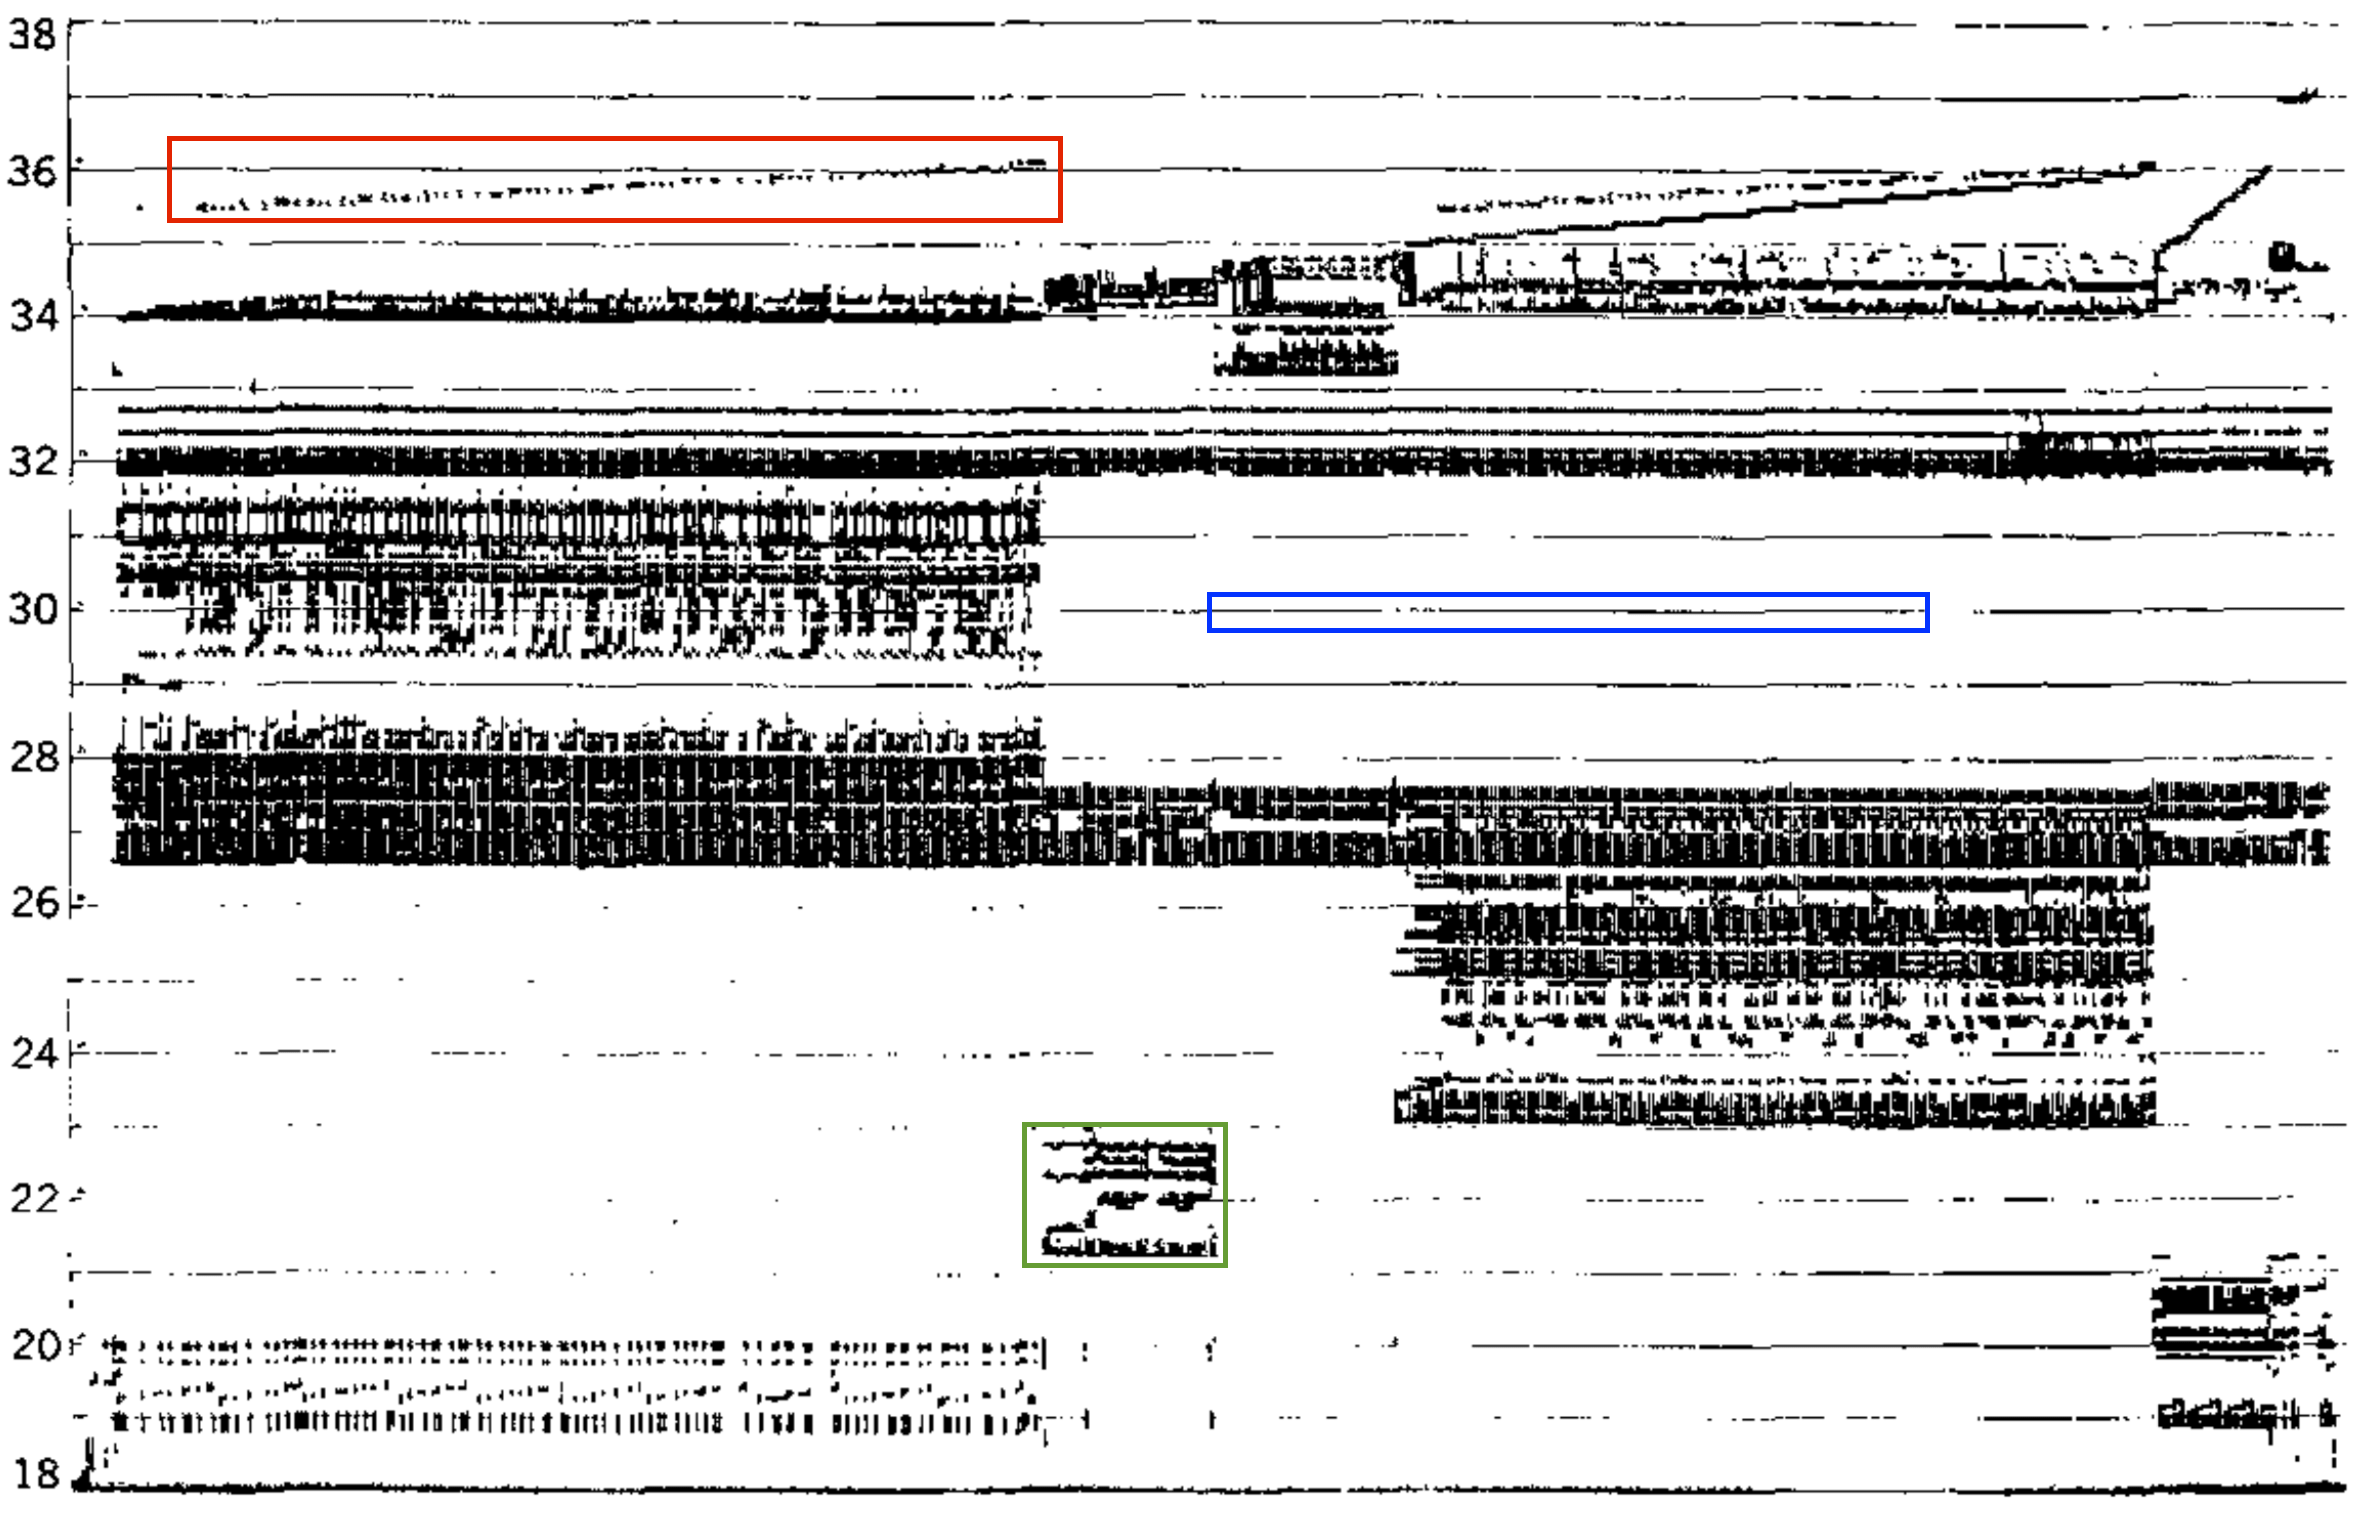
\includegraphics[width=14cm]{images/cpu_locality.png}
            \caption{ Évolution du numéro des pages accédé (axe des ordonnées) en fonction du temps (axe des abscisses) tiré de \cite{Hatfield:1971}. Les accès encadrés en bleu ont une localité temporelle. Les accès encadrés en vert ont une localité spatiale. Les accès encadrés en rouge ne profitent d'aucune localité. 
            \label{pic_cpu_locality}}
        \end{figure}

    
    \subsubsection{Saturation du bus mémoire}
    %%%%%%%%%%%%%%
    
        Les performances des applications étant principalement limitées par le bus mémoire, il est important que ce dernier soit utilisé à son maximum. On parle alors de \textit{saturation} du bus mémoire. Pour comprendre le lien entre la saturation du bus et la latence mémoire nous utilisons la loi de Little .
        
        \paragraph{Loi de Little \cite{Little_1961}.} \label{sec:loidelittle} Cette loi énoncée en 1961, est utilisée dans la théorie des files d'attente. Elle sert à caractériser le nombre de personnes $N$ dans un système stable (comme une file d'attente), en fonction du temps de traitement $L$ et du débit moyen de client $T$. Le nombre de personnes dans la file peut être calculé par la loi de Little (voir \autoref{eq:little}). Ainsi, pour réduire le temps d'attente d'un client dans une file, il faut soit réduire le nombre de personnes présentes simultanément dans la queue, ou augmenter la cadence de traitement.
        
        \begin{equation} \label{eq:little}
            N = L \times T
        \end{equation}
        
        Bien qu'en apparence éloignée du domaine des ordinateurs, cette loi est fondamentale pour comprendre la performance du bus mémoire. Le bus mémoire peut être vu comme une file d'attente dont les clients sont des requêtes mémoires en attente, le temps de traitement est la latence mémoire et le débit représente la bande passante mémoire. La latence et le débit mémoire sont donnés par les caractéristiques de l'architecture. Le but du programmeur est d'utiliser la performance maximale du bus mémoire. Il doit pour cela générer suffisamment de transactions mémoires permettant sa saturation.
        
        Prenons l'exemple d'un bus mémoire ayant une bande passante de 128 GB/s transférant des lignes de cache de 64 bytes et une latence mémoire de 100 ns. Son débit est alors de 2 lignes de cache par nanoseconde. Avec la loi de Little, il est possible de calculer le nombre de requêtes mémoires concurrentes nécessaires pour saturer la bande passante mémoire. Dans notre exemple, il est égal à $100 \times 2 = 200$ transactions (voir \autoref{pic_cpu_littlelaw}). 
        Si le code, ou l’architecture n’est pas capable de générer, au minimum, 200 requêtes mémoires chaque nanoseconde, le bus mémoire ne pourra jamais être saturé. Un autre impact est que si un processeur est capable de les générer, lui ajouter des coeurs, ne permettra pas d’obtenir de meilleures performances du bus. Pour certains codes limités par la bande passante, il peut être intéressant d’éteindre certains coeurs pour limiter la consommation du processeur sans affecter la performance du code.
        
        
        \begin{figure}
            \center
            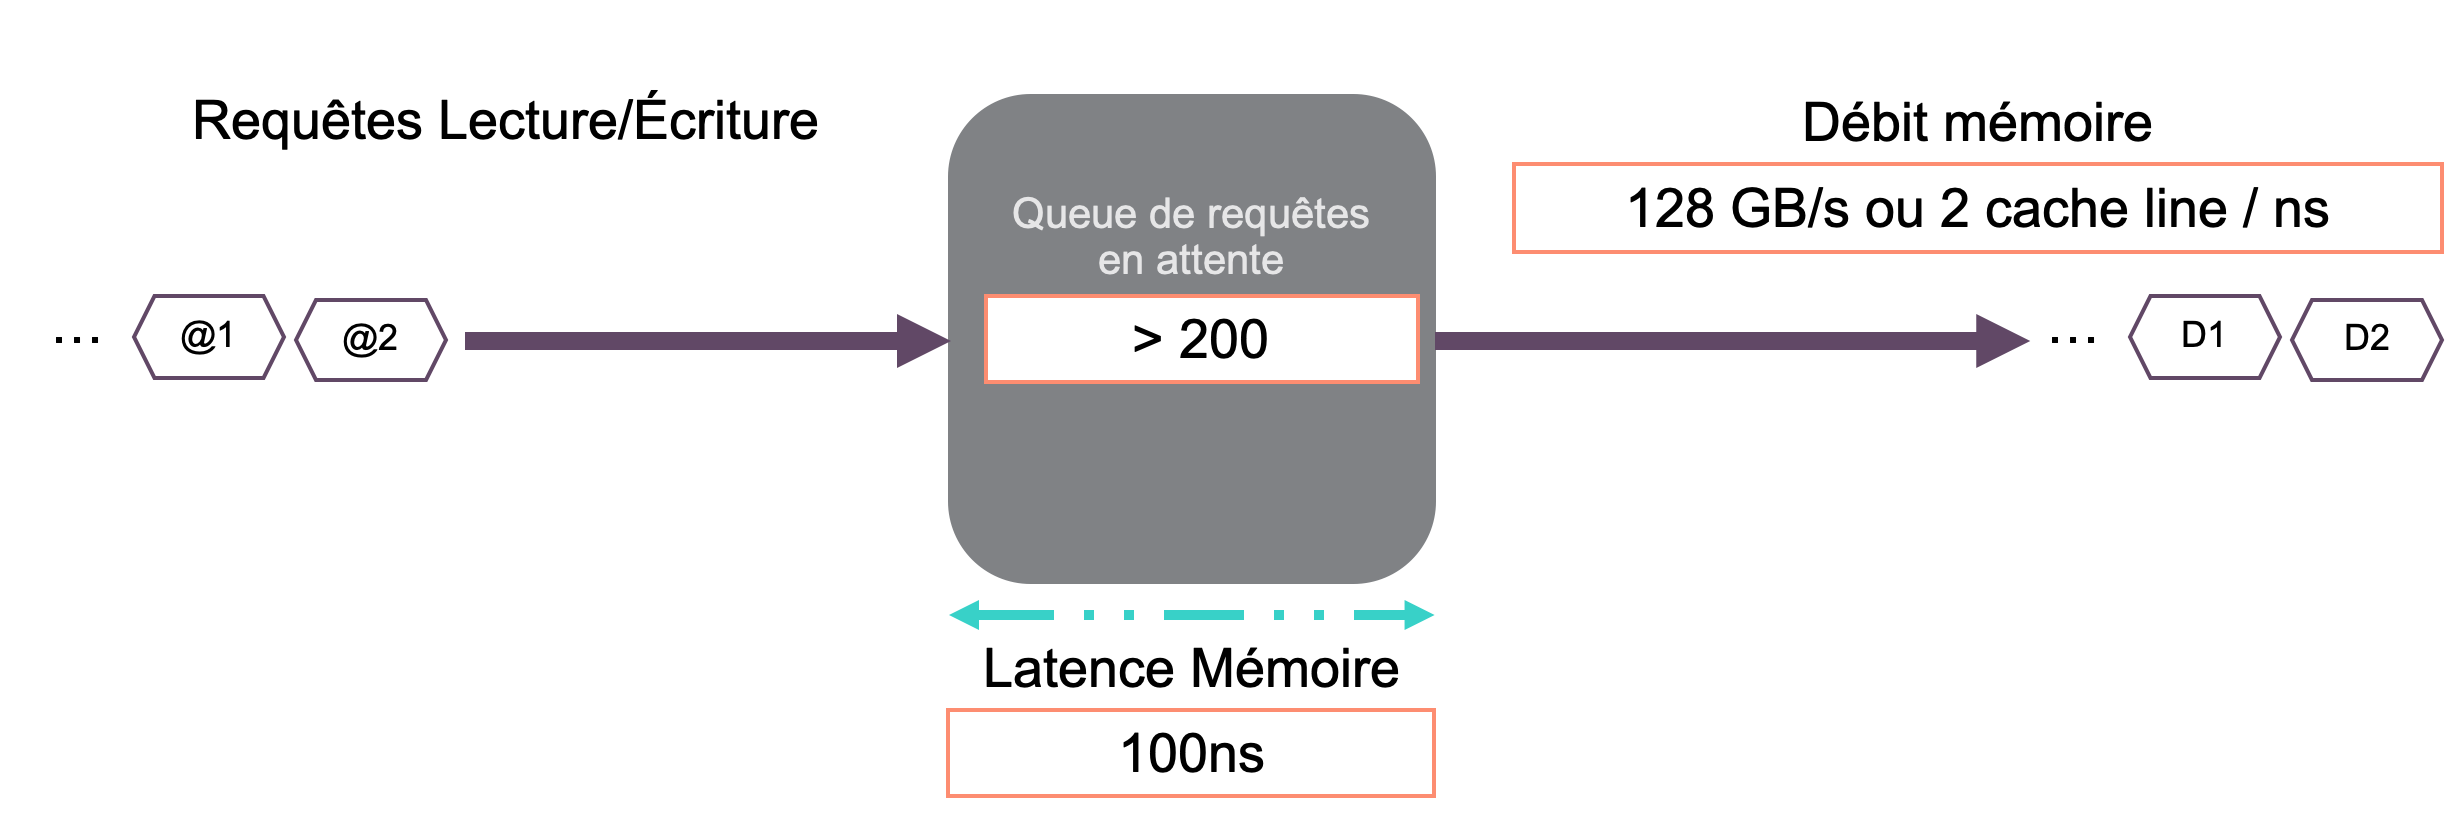
\includegraphics[width=12cm]{images/cpu_littlelaw.png}
            \caption{ La loi de Little permet de calculer le nombre de requêtes mémoires nécessaire pour saturer le bus mémoire. Pour un bus mémoire de 128 GB/s et une latence mémoire de 100 ns, il faut qu'il y ait plus de 200 requêtes mémoires en attente pour que le bus soit saturé.
            \label{pic_cpu_littlelaw}}
        \end{figure}
        
        Cette loi à un impact direct sur les architectures modernes utilisant des mémoires HBM. Ces mémoires ont des latences d’accès un peu plus faible dû à leur proximité du processeur. Les débits mémoires sont eux aussi bien meilleurs. La loi de Little, implique que le nombre d’accès mémoire concurrents nécessaires pour saturer ces bus va fortement augmenter. Malheureusement, la microarchitecture actuelle des processeurs n’est pas forcément adaptée à de telles évolutions. Ainsi, nous avons rencontré des architectures incapables de saturer la bande passante mémoire disponible. 

%%%%%%%%%%%%%%%%%%%%%%%%%%%%%%%%%%%%%%%%%%%%%%%%%%%%%%%%%%%%%%%%%%%



\subsection{Caches} \label{sec:cache}
%%%%%%%%%%%%%%%%%%%%%%%%%%%%%%%%%%%%%%%%%%%%%%%%%%%%%%%%%%%%%%%%%%%
%%%%%%%%%%%%%%%%%%%%%%%%%%%%%%%%%%%%%%%%%%%%%%%%%%%%%%%%%%%%%%%%%%%
    
    %intro
    C'est en 1965 que les premières mémoires caches sont présentées sous le nom de \textit{slave memory} \cite{wilkes1965slave}. Leur temps d'accès est 4 à 20 fois plus rapide que celui de la mémoire principale. Cependant, leur taille est très réduite (quelques MiB) comparée à celle de la mémoire principale (plusieurs GiB). Les caches utilisent généralement de la mémoire SRAM.
    
    %performance
    Ce niveau de mémoire a été implémenté pour réduire, du point de vue du processeur, l'écart de performance entre ses unités de calculs et celles de la mémoire centrale. Leur apport de performance vient de la capacité des programmes à réutiliser des données déjà présentes dans le cache, évitant un accès à la mémoire centrale beaucoup plus long. Lorsque le processeur doit accéder à une donnée, il commence par la chercher dans le premier niveau de cache, si elle s’y trouve, son temps d'accès est très rapide (événement \textit{cache hit}). Si ce n'est pas le cas (événement \textit{cache miss}), il réalise alors une copie de la zone mémoire la contenant dans le cache. La zone mémoire copiée est appelé \textit{ligne de cache}. Si par la suite, cette donnée ou une donnée appartenant à la même ligne de cache devait être à nouveau accédée, leur temps d'accès serait alors drastiquement réduit. Ce mécanisme est transparent pour l'utilisateur, bien que pour des questions de performances il doive être conscient de son existence (voir \autoref{sec:locality}). 
    
    %taille vs performance
    La taille de chaque niveau de cache varie pour les raisons expliquées en introduction de cette partie. À cela vient s'ajouter la notion de performance qui est liée à leur taille. Un cache de grande capacité aura plus de chance de contenir la donnée dont le processeur a besoin, améliorant ainsi la performance moyenne du programme. 
    
    %Un cache est une mémoire associative. Pour accéder à son contenu, il faut utiliser une clef associative. La clef est constituée de l'adresse en mémoire centrale de l'instruction ou de la donnée.
    
    Pour allier les avantages et contourner les inconvénients, les processeurs utilisent non pas un, mais plusieurs niveaux de caches de tailles différentes.
    Le premier niveau de cache est généralement séparé en deux zones mémoire: l'une contenant les instructions et l'autre les données. C'est le seul niveau de la hiérarchie qui stocke différemment les données et les instructions. Sur les processeurs récents, le premier et le deuxième niveau de cache est privé à chaque coeur. Un troisième et parfois un quatrième niveau de cache est partagé entre les différents coeurs du processeur. La \autoref{pic:cache_hierarchy} représente une telle architecture pour un processeur à 4 coeurs. Le partage d'un ou plusieurs niveaux de caches entre différents coeurs à certains bénéfices en programmation parallèle. La communication entre les coeurs est plus rapide, ainsi que la migration d'un thread entre deux coeurs partageant un même niveau de cache. Cependant, cela introduit de la complexité pour la cohérence des caches (voir \autoref{sec:cache_coherence}).
    
    
    \begin{figure}
        \center
        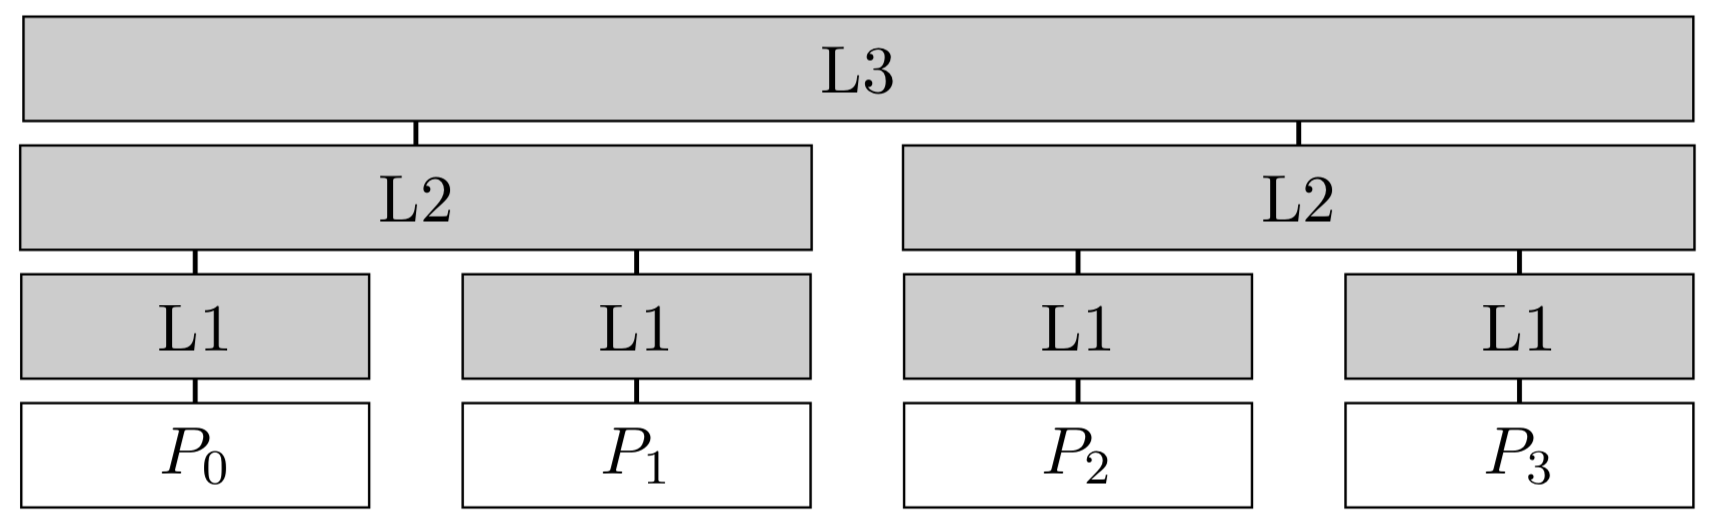
\includegraphics[width=8cm]{images/cache_hierarchy.png}
        \caption{\label{pic:cache_hierarchy} Organisation d'une hiérarchie de caches à trois niveau sur un processeur à 4 coeurs (source \cite{putigny2014benchmark}).}
    \end{figure}
    
    
        
        
    \subsubsection{Propriété d'inclusion}
    %%%%%%%%%%%%%%%%%%%%%%%%%%%%%%%%%%%%%%%%%%%%%%%%%%%%%%%%%%%%%%%%%%%
        
        Lorsqu'une donnée est chargée depuis la mémoire, le processeur doit la stocker dans le cache. La manière de stocker l'information  varie en fonction de la propriété d'inclusion du processeur:
        \begin{itemize}
            \item Un cache est dit inclusif, si une donnée peut se trouver dans plusieurs niveau de cache au même moment (voir \autoref{pic:InclusivePolicy}). Cette politique d'inclusion a un désavantage lorsqu'elle est utilisée sur des systèmes multi-coeurs. En effet, lorsqu'une donnée doit être retirée d'un niveau de cache, le processeur doit aussi l'enlever des niveaux de caches inférieurs alors que celle-ci pouvait être actuellement utilisé par un autre coeur.
        
            \item Un cache est dit exclusif, si à un instant donné, une donnée ne peut pas être à stockée à plusieurs endroits dans la hiérarchie de cache (voir \autoref{pic:ExclusivePolicy}). L'avantage des caches exclusif est leur capacité de stocker plus de données, car une ligne de cache ne se trouve jamais à deux endroits à la fois de la hiérarchie de cache. Cependant, lors d'un \textit{hit} dans le cache L2, le processeur doit échanger la ligne entre les deux niveaux de cache L1 et L2, plus long qu'une simple copie.
        \end{itemize}
        Les processeurs récents peuvent implémententer les deux politiques d'inclusion. Le processeur Intel Sandy Bridge a un cache L3 inclusif tandis que les caches L1 et L2 sont non-inclusif. 
        
        
        \begin{figure}
            \centering
            \begin{subfigure}[b]{0.45\linewidth}
                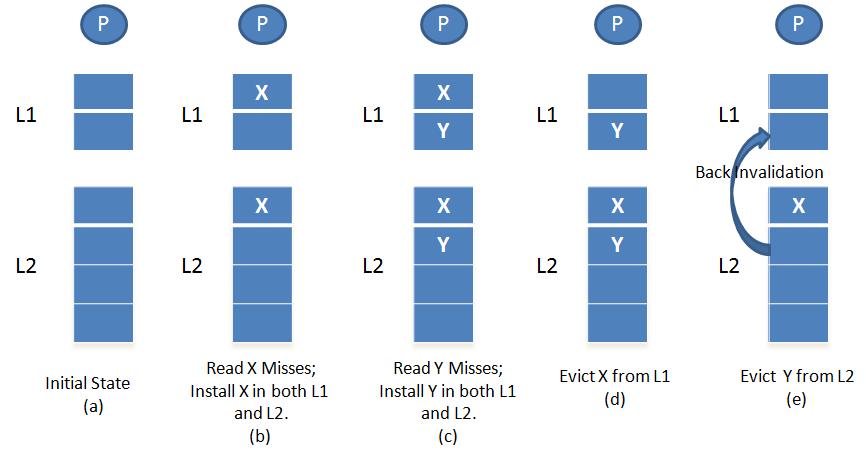
\includegraphics[width=\linewidth]{images/InclusivePolicy.png}
                \caption{Inclusive}
                \label{pic:InclusivePolicy}
            \end{subfigure}
            ~ %add desired spacing between images, e. g. ~, \quad, \qquad, \hfill etc. 
              %(or a blank line to force the subfigure onto a new line)
            \begin{subfigure}[b]{0.45\linewidth}
                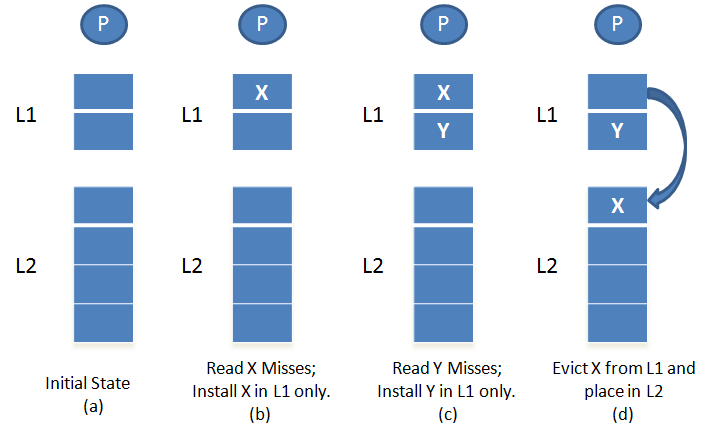
\includegraphics[width=0.85\linewidth]{images/ExclusivePolicy.png}
                \caption{Exclusive}
                \label{pic:ExclusivePolicy}
            \end{subfigure}
            \caption{\label{fig:cacheinclusionpolicy} Exemple de deux propriétés d'inclusion de la hiérarchie de cache (source \cite{wikipedia_2019}). }
        \end{figure}
        

    \subsubsection{Politique de placement: associativité}
    %%%%%%%%%%%%%%%%%%%%%%%%%%%%%%%%%%%%%%%%%%%%%%%%%%%%%%%%%%%%%%%%%%%

        La performance d'un cache ne vient pas seulement de la technologie utilisée pour sa construction. En effet, lorsqu'une donnée est accédée, le cache doit vérifier si la donnée est présente ou non dans le niveau de cache demandé. Il faut que l'algorithme de comparaison permettant de la trouver soit le plus rapide possible. Pour cela, les architectes utilisent généralement une fonction de \textit{hash} permettant d'attribuer un emplacement dans le cache en fonction de l'adresse mémoire de la ligne de cache. Si la ligne de cache ne se trouve pas à l'emplacement (ou les emplacements) calculé, c'est quelle n'est pas présente dans ce niveau de cache. Les trois politiques de placement les plus utilisées sont:
        \begin{itemize}
            \item le mappage  \textit{direct} - \autoref{pic:cachemappage_direct}
            \item le mappage \textit{fully associative} - \autoref{pic:cachemappage_fully}
            \item le mappage \textit{set assiociative} - \autoref{pic:cachemappage_setasso}
        \end{itemize}
        
        %\clearpage
            \begin{figure}
            
                \centering
                \begin{subfigure}[b]{0.35\linewidth}
                    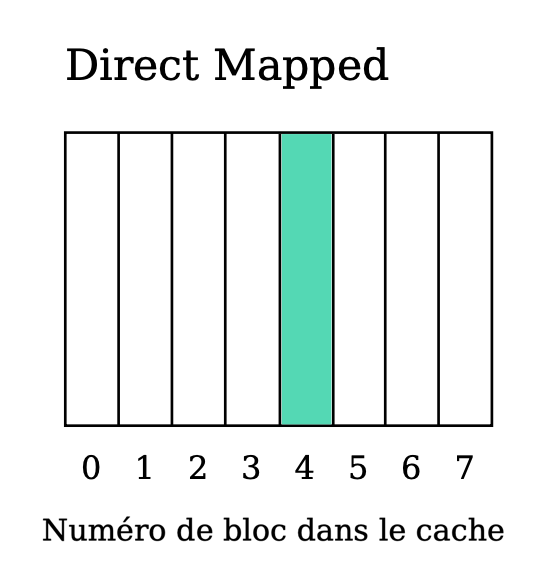
\includegraphics[width=5cm]{images/cache_direct.png}
                    \caption{Un seul emplacement par ligne de cache \cite{Meunier2017}).}
                    \label{pic:cache_direct_pti}
                \end{subfigure}
                ~ %add desired spacing between images, e. g. ~, \quad, \qquad, \hfill etc. 
                  %(or a blank line to force the subfigure onto a new line)
                \begin{subfigure}[b]{0.60\linewidth}
                    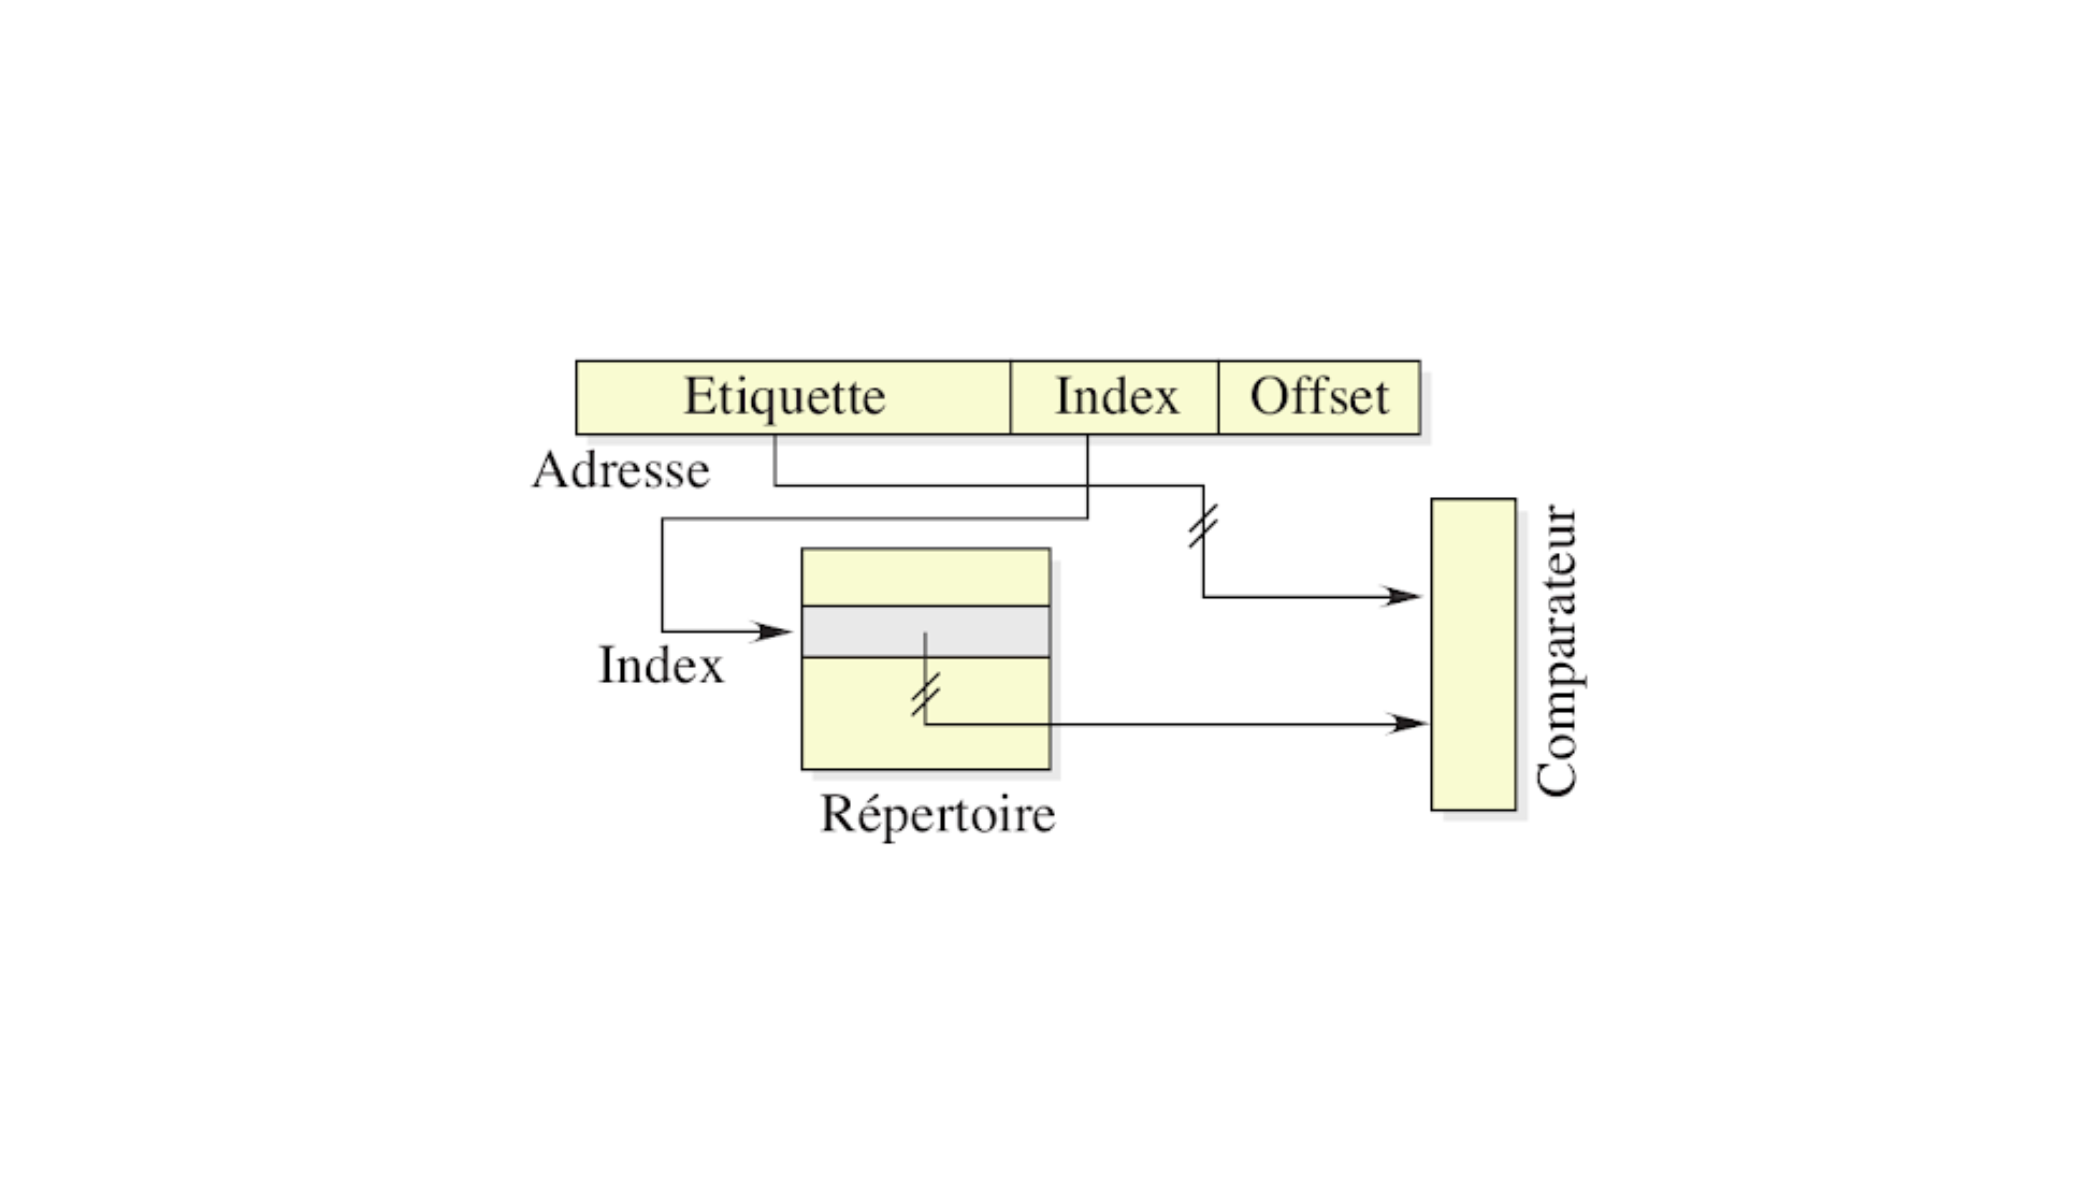
\includegraphics[width=\linewidth]{images/cache_circuit-direct.png}
                    \caption{Le cache pleinement associatif nécessite d'avoir un comparateur pour chacune des lignes du cache (extrait de l'ouvrage \cite{Blanchet2013}).}
                    \label{pic:cache_circuit-direct}
                \end{subfigure}
                \caption{Cache à correspondance directe}\label{pic:cachemappage_direct}
            %\end{figure}
                        \vspace*{\floatsep}% https://tex.stackexchange.com/q/26521/5764


            %\begin{figure}
                \centering
                \begin{subfigure}[b]{0.35\linewidth}
                    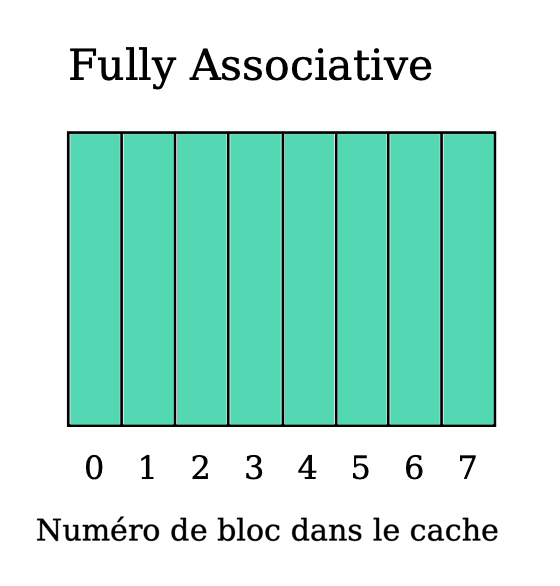
\includegraphics[width=5cm]{images/cache_asso.png}
                    \caption{Une ligne de cache peut être à n'importe quel emplacement \cite{Meunier2017}).}
                    \label{pic:cache_asso}
                \end{subfigure}
                ~ %add desired spacing between images, e. g. ~, \quad, \qquad, \hfill etc. 
                  %(or a blank line to force the subfigure onto a new line)
                \begin{subfigure}[b]{0.60\linewidth}
                    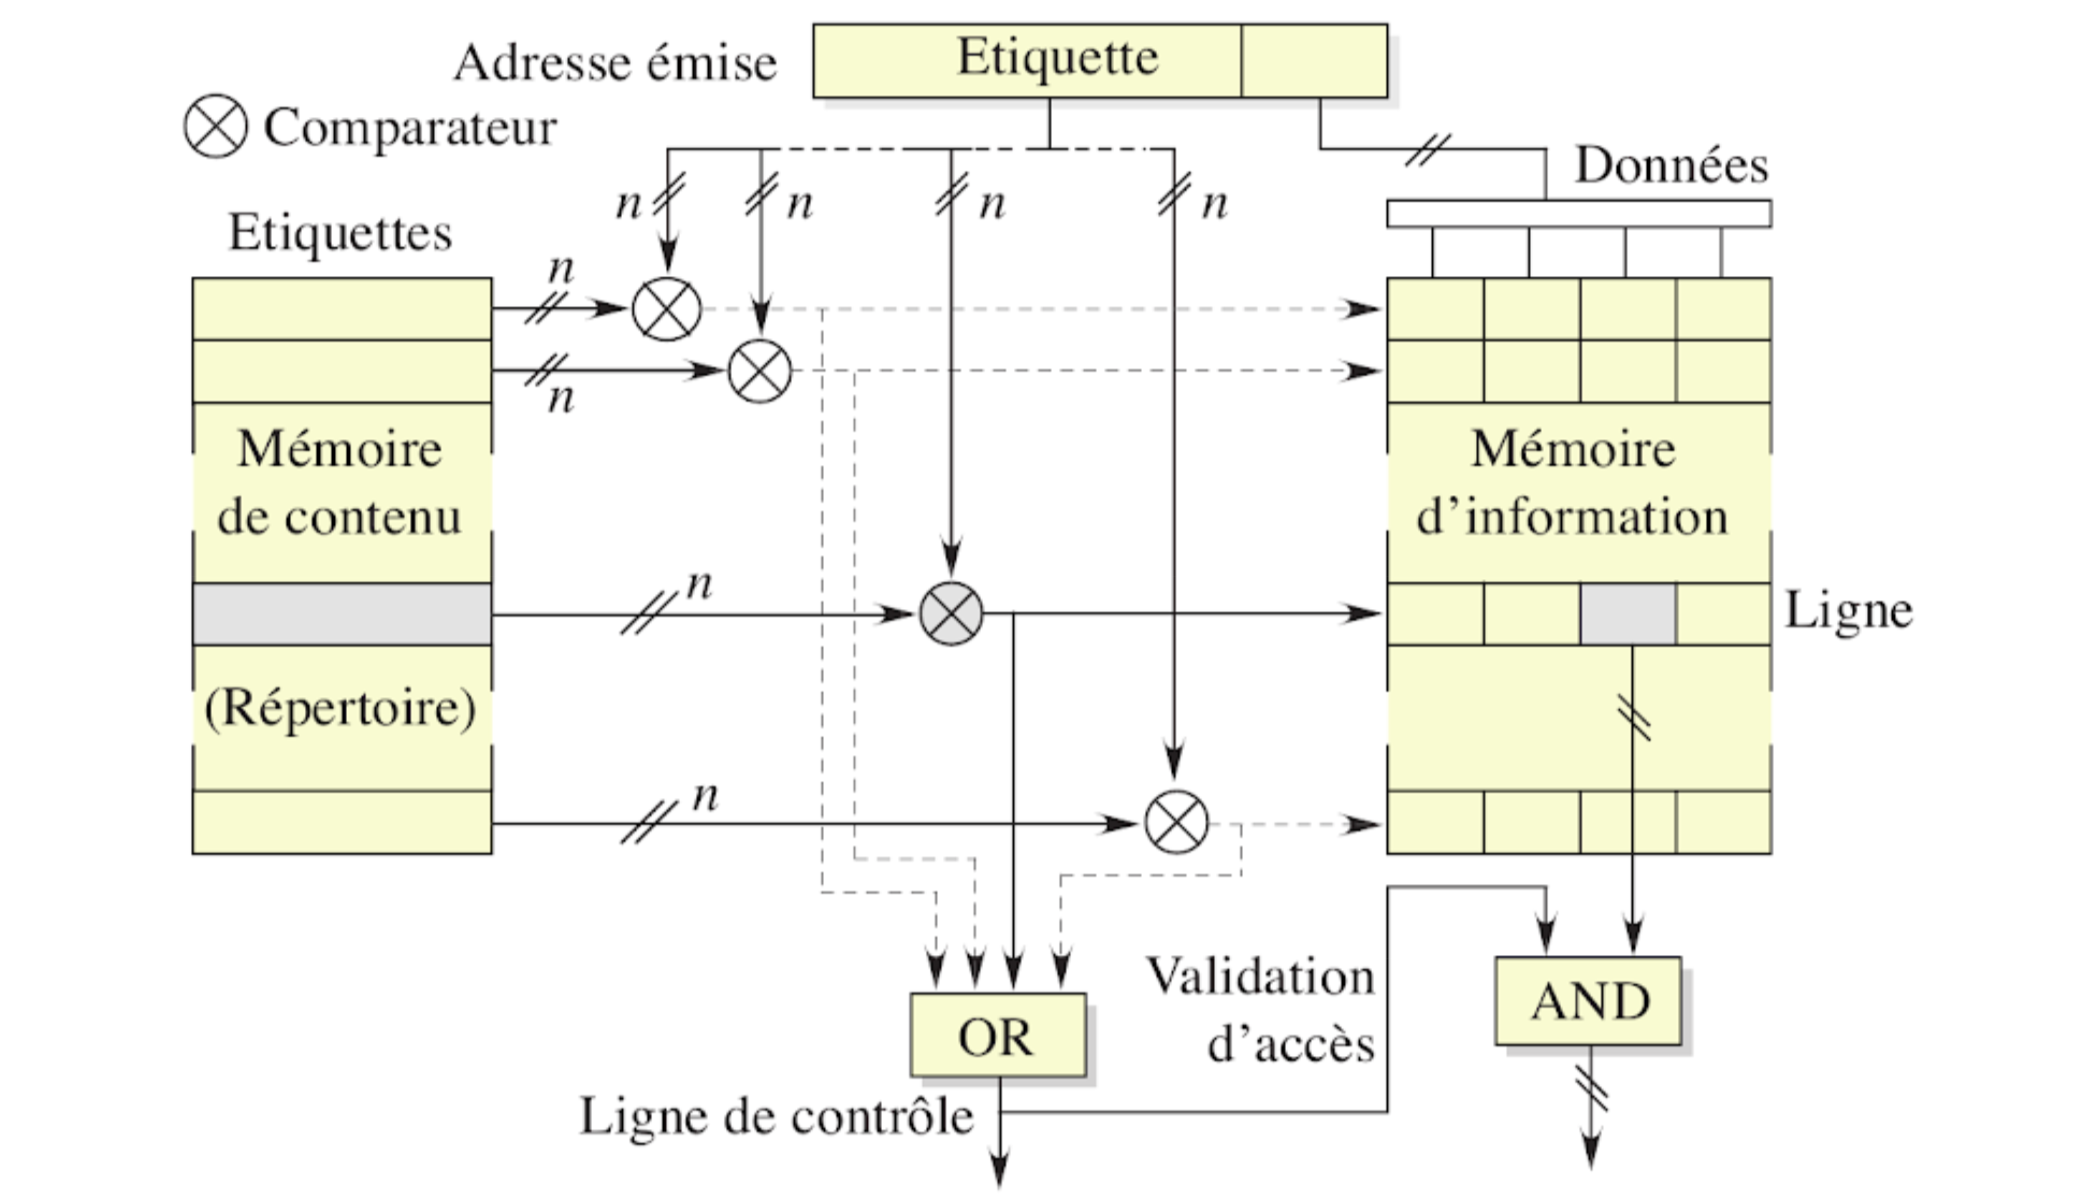
\includegraphics[width=\linewidth]{images/cache_circuit-fully-associative.png}
                    \caption{Le cache pleinement associatif nécessite d'avoir un comparateur pour chacune des lignes du cache (extrait de l'ouvrage \cite{Blanchet2013}).}
                    \label{pic:cache_circuit-fully-associative}
                \end{subfigure}
                \caption{Cache pleinement associatif}\label{pic:cachemappage_fully}
            %\end{figure} 
            
                   \vspace*{\floatsep}% https://tex.stackexchange.com/q/26521/5764

           %\begin{figure}
                \centering
                \begin{subfigure}[b]{0.35\linewidth}
                    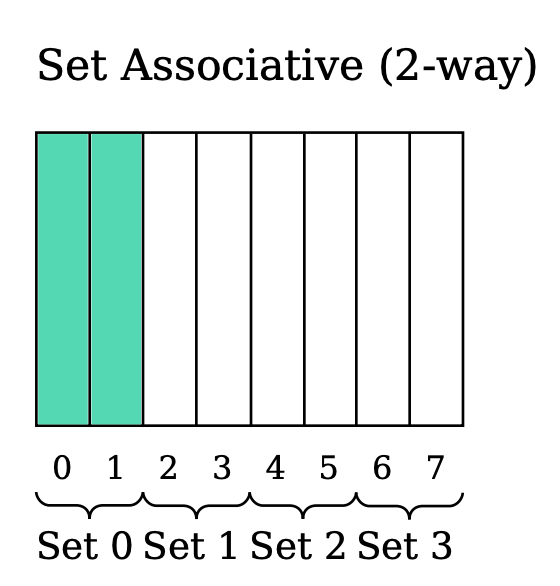
\includegraphics[width=5cm]{images/cache_asso_2way.png}
                    \caption{Une ligne de cache peut être à un nombre restreint d'emplacement \cite{Meunier2017})}
                    \label{pic:cache_asso_2way}
                \end{subfigure}
                ~ %add desired spacing between images, e. g. ~, \quad, \qquad, \hfill etc. 
                  %(or a blank line to force the subfigure onto a new line)
                \begin{subfigure}[b]{0.60\linewidth}
                    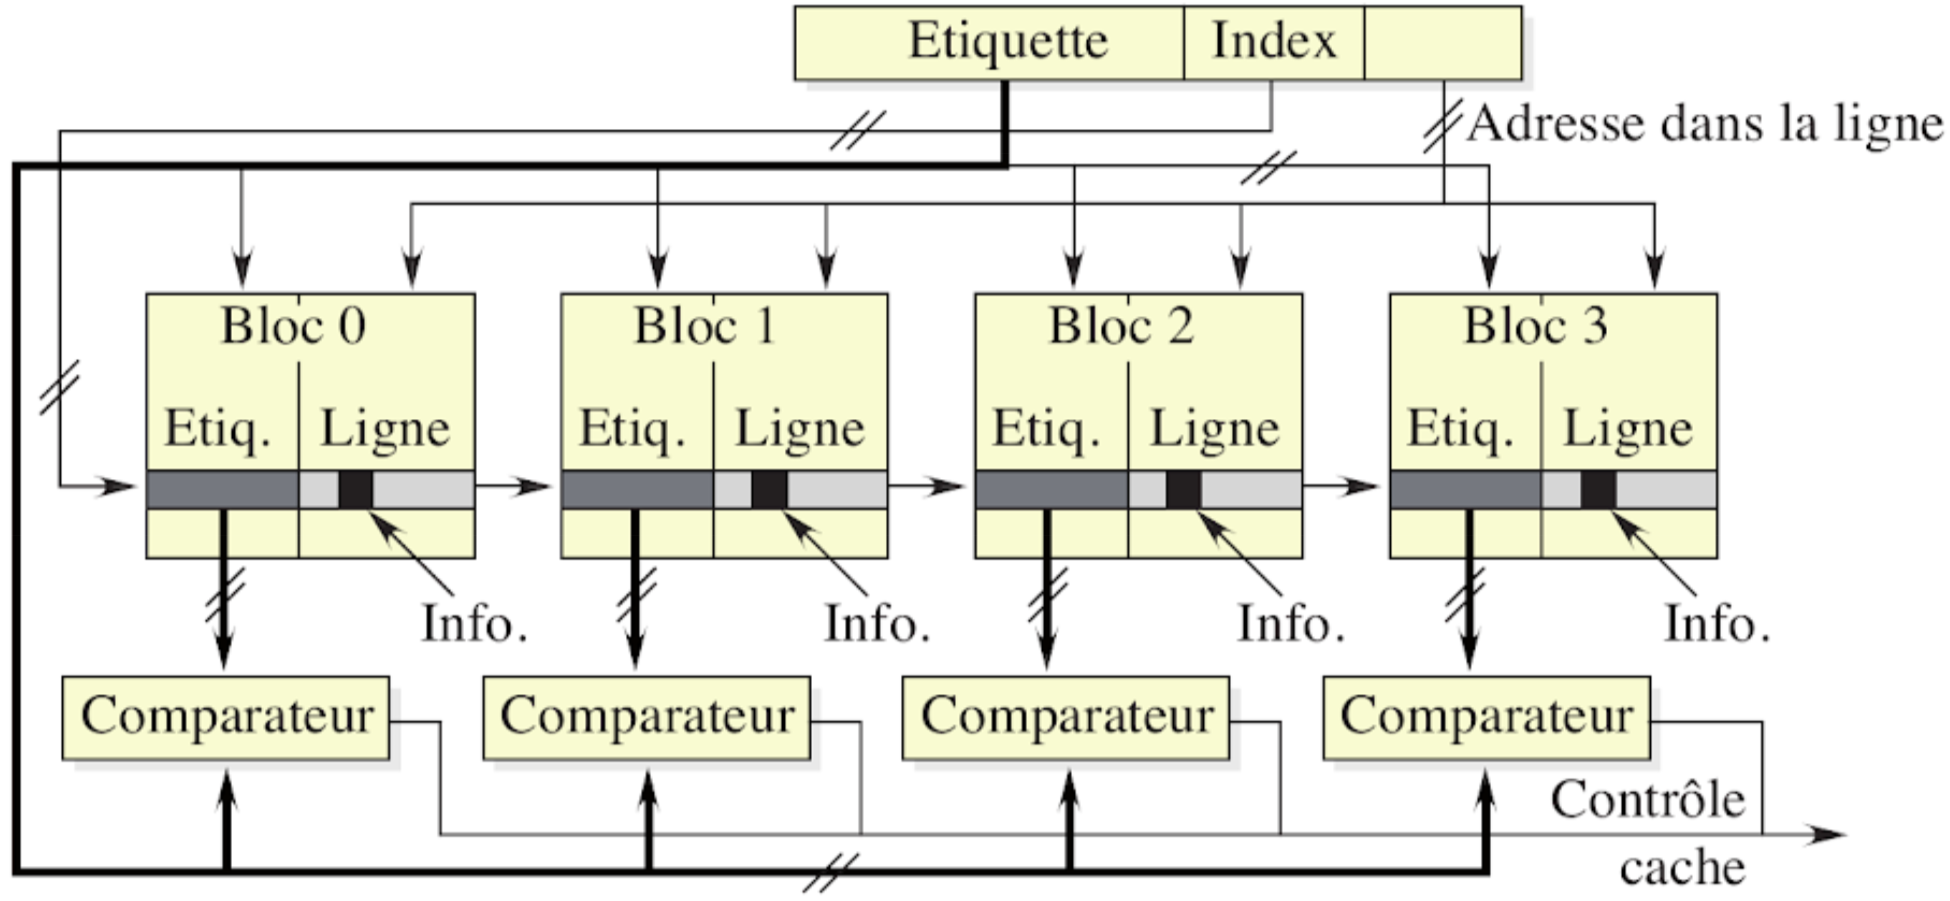
\includegraphics[width=\linewidth]{images/cache_circuit-set-associative.png}
                    \caption{Le cache N-associatif associe les deux architectures des caches direct et pleinement associatif. Ce sont plusieurs caches directs montés en parallèles (extrait de l'ouvrage \cite{Blanchet2013}).}
                    \label{pic:cache_circuit-set-associative}
                \end{subfigure}
                \caption{Cache N-associatif}\label{pic:cachemappage_setasso}
        \end{figure}
       
       
        

        \paragraph{Cache à correspondance directe (\textit{direct-mapped cache})} 
            
            Cette politique utilise une fonction simple pour déterminer l'emplacement du cache à utiliser. Une partie des bits le l'adresse de la ligne de cache est utilisée pour déterminer la ligne à utiliser (\textit{index}) par exemple à l'aide d'une opération modulo. L'autre partie est utilisée pour déterminer le décalage dans cette ligne (\textit{offset}) (voir  \autoref{fig:cachemappage}). Cette méthode est très rapide, mais peut avoir des performances catastrophiques. Un algorithme faisant des sauts en mémoire d'une certaine taille pourrait n'utiliser qu'une seule ligne du cache, le rendant totalement inefficace. Comparé aux caches associatifs, le mappage direct est plus simple à implémenter, car un seul comparateur est nécessaire pour déterminer la ligne de cache à utiliser (voir \autoref{pic:cache_direct_coucou}).
 
            \begin{figure}
                \centering
                \begin{subfigure}[b]{0.45\linewidth}
                    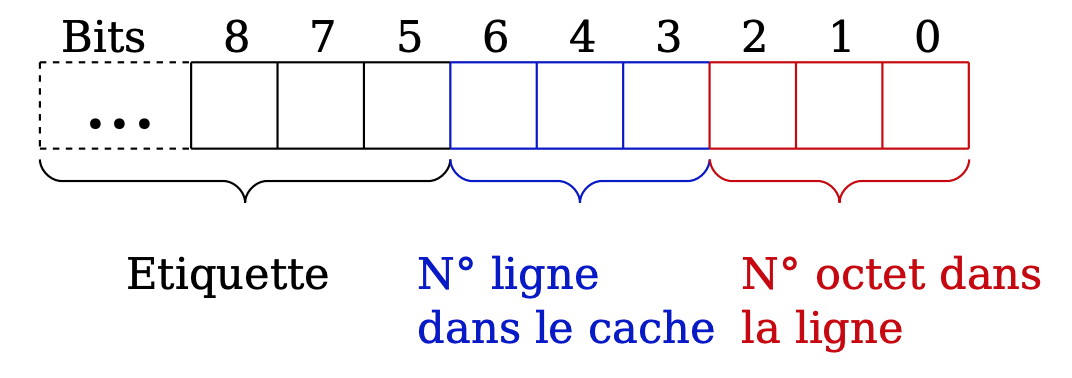
\includegraphics[width=\linewidth]{images/cache_calcul.png}
                    \caption{Calcul de l'emplacement (index de la ligne et décalage) pour un mappage direct}
                    \label{pic:cache_calcul}
                \end{subfigure}
                ~ %add desired spacing between images, e. g. ~, \quad, \qquad, \hfill etc. 
                  %(or a blank line to force the subfigure onto a new line)
                \begin{subfigure}[b]{0.45\linewidth}
                    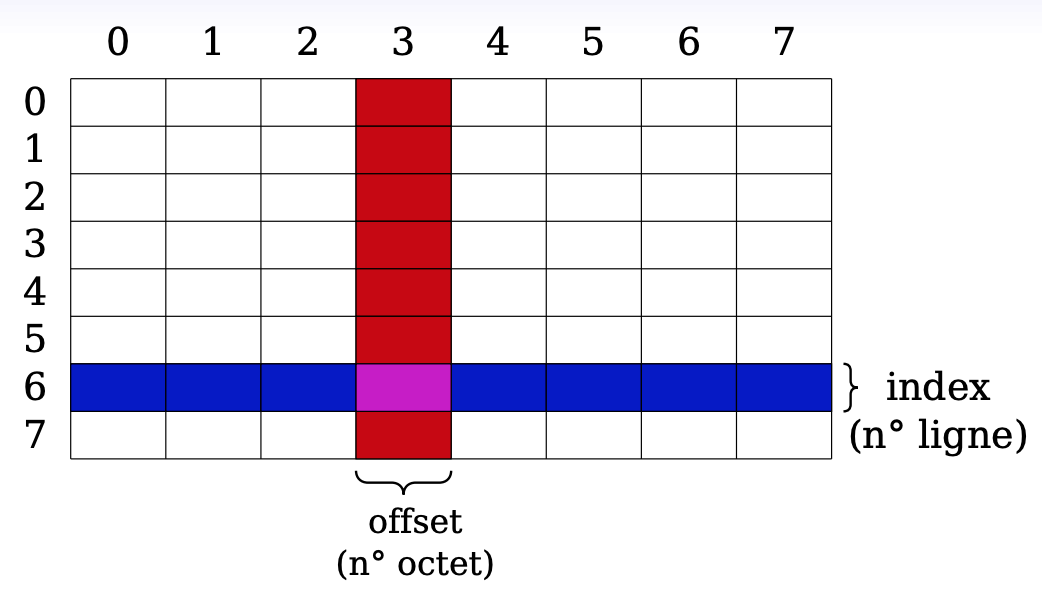
\includegraphics[width=\linewidth]{images/cache_direct_coucou.png}
                    \caption{Emplacement de la ligne calculée dans le cache ou sera stockée la ligne de cache.}
                    \label{pic:cache_direct_coucou}
                \end{subfigure}
                \caption{Exemple du calcul de l'emplacement de la ligne de cache lors d'un mappage direct à partir de l'adresse de la ligne de cache à stocker (source \cite{Meunier2017}). }\label{fig:cachemappage}
            \end{figure}
        
        \paragraph{Cache pleinement associatif (\textit{fully associative cache})} 
            
            Cette politique remédie à l'inconvénient relevé concernant la correspondance directe, en permettant à une ligne de cache d'être stockée à n'importe quel empl\autoref{pic:cachemappage_fully}). Ainsi, la totalité du cache peut être utilisée. Cependant, cette technique a le désavantage d'être très lente. En effet, une ligne de cache pouvant se trouver à n'importe quel index du cache, il faut tous les comparer pour vérifier sa présence ou non. Pour faire cette comparaison en parallèle, il faudrait implémenter autant de comparateurs que de ligne dans le cache, complexifiant grandement le cache.
            
            
            
        \paragraph{Cache N-associatif (\textit{N-way set associative cache})} 
            
            Cette politique permet de réduire le nombre de comparateurs qu'un cache associatif devrait posséder pour être rapide. Ceci est réalisé en regroupant les lignes du caches potentiellement adressable pour une ligne de cache en groupe (\textit{set}). L'exemple de la \autoref{pic:cache_asso_2way} utilise un cache à 4 set regroupant 2 lignes de caches, appelé \textit{2-way associative}. Il ne faut plus que 4 comparateurs pour déterminer si une ligne appartient à un des \textit{set}. Les mappages par association sont plus lents que le mappage direct, car il faut trouver où se trouve la ligne de cache (si présente) dans un sous ensemble de ligne de cache plus ou moins grand. Pour accélérer la recherche de la présence ou non d'une ligne de cache, le traitement peut être réalisé en parallèle dans les différents \textit{sets} par l'utilisation de plusieurs comparateurs (4 dans la \autoref{pic:cache_circuit-set-associative}). 
        
            La propriété principale d'un cache est sa capacité à conserver les données pour de futurs accès. Un cache de 8 MB à 2 sets associatifs peut sauver jusqu'à 44\% des \textit{miss} comparé à un cache à correspondance direct \cite{Drepper2007}. Sur les architectures récentes Intel Skylake, les caches utilisent entre 8 et 16 associativités, pouvant varier entre les différents niveaux. 
       
       
       
        \iffalse
            \textbf{todo check emplacement}
            \begin{figure}
                \begin{subfigure}[t]{0.99\linewidth}\centering
                    \includegraphics[width=0.7\linewidth, trim = 0cm 10cm 0cm 2cm]{images/cache_circuit-direct.png}
                    \caption{Le cache pleinement associatif nécessite d'avoir un comparateur pour chacune des lignes du cache}
                    \label{pic:cache_circuit-direct}
                    \vspace{1cm}
                \end{subfigure}
                
                \begin{subfigure}[t]{\linewidth}\centering
                    \includegraphics[width=0.7\linewidth]{images/cache_circuit-fully-associative.png}
                    \caption{Le cache pleinement associatif nécessite d'avoir un comparateur pour chacune des lignes du cache}
                    \label{pic:cache_circuit-fully-associative}
                    \vspace{.5cm}
                \end{subfigure}
                
                \begin{subfigure}[t]{\linewidth}\centering
                    \includegraphics[width=0.7\linewidth]{images/cache_circuit-set-associative.png}
                    \caption{Le cache N-associatif associe les deux architectures des caches direct et pleinement associatif. Ce sont plusieurs caches directs montés en parallèles.}
                    \label{pic:cache_circuit-set-associative}
                \end{subfigure}
                
                \caption{Schémas des trois modèles de cache utilisés (tirés de l'ouvrage \cite{Blanchet2013}).}\label{fig:cache_schema}
            \end{figure}
        
                
    
            
    
        
        \fi

    \subsubsection{Politique de remplacement}
    %%%%%%%%%%%%%%%%%%%%%%%%%%%%%%%%%%%%%%%%%%%%%%%%%%%%%%%%%%%%%%%%%%%

        Que ce soit pour le mappage \textit{fully associative} ou \textit{set associative}, une ligne de cache peut être stockée dans plusieurs lignes du cache. Pour déterminer laquelle choisir pour y placer la ligne de cache, différentes stratégies peuvent être utilisées, appelées \textit{politique de remplacement}. L'objectif de ces politiques est de maximiser l'utilisation du cache en prévoyant et en anticipant les futures lignes à être accéder pour ne pas les supprimer du cache. Il existe de nombreuses politiques de remplacement, chacune ayant ses avantages et ses inconvénients \cite{wikipedia2_2019}: FIFO, LIFO, LRU, TLRU, MRU, PLRU, RR, SLRU, LFU, LFRU, LFUDA, LIRS, ARC, CAR, MQ. La politique choisie à un réel impacte sur les performances de l'application. Pour la choisir, il faut trouver un compromis entre la performance et la complexité apportée par sa mise en place. Dans le cas du mappage \textit{direct}, la ligne de cache présente à l'emplacement calculé est forcément remplacée et ne nécessite pas d'avoir une politique de remplacement. Il existe deux familles de politiques de remplacement. La première famille regroupe les politiques de remplacements qui tiennent compte de l'utilisation des ligne de cache (LRU, FIFO). Ce sont généralement les politiques les plus efficaces. La deuxième famille est celle des politiques aléatoires (\textit{random}, \textit{round robin}) qui ne tiennent pas compte de l'utilisation des données et choisissent une ligne aléatoirement à remplacer. Ces politiques sont performantes en termes de rapidité d'exécution, car le choix ne se fait que sur une fonction aléatoire. Cependant, \cite{Al-Zoubi:2004:PEC:986537.986601} montrent que ces techniques utilisent 22\% moins bien le cache, impactant les performances des applications.
        
        
        \paragraph{Least Recently Used} 
        
            ou LRU remplace la ligne de cache la moins récemment utilisée. Les numéros des lignes utilisées sont stockés dans une pile suivant la date de leur dernière utilisation. La pile est mise à jour lorsqu'une nouvelle donnée est stockée dans le cache en empilant son adresse au sommet de la pile. De même, lors d'un \textit{hit}, la ligne de cache référencé est stockée elle aussi en sommet de pile. Cette méthode à un inconvénient pour certains types d'accès, notamment les parcours de tableau. Imaginons un cache pouvant contenir 4 lignes. Le double parcours d'un tableau mesurant 5 lignes de caches a,b,c,d,e aura les accès mémoire suivants: a,b,c,d,e a,b,c,d,e. Le deuxième accès au tableau ne profitera pas du cache, car chaque ligne de cache est remplacée au fur et mesure du parcours du tableau. Des améliorations ont été apportées pour corriger ce problème, comme l'introduction d'un répertoire image \cite{Stone:1987:HCA:31845} qui garde une trace des groupes de lignes de cache utilisées ensemble pour prévoir les accès similaires et anticiper leur accès.

    
    \subsubsection{Stratégie de cache: lecture et écriture}
    %%%%%%%%%%%%%%%%%%%%%%%%%%%%%%%%%%%%%%%%%%%%%%%%%%%%%%%%%%%%%%%%%%%

        Le cache est une zone mémoire qui évolue en fonction des accès mémoires. Son fonctionnement lors d'un accès (en lecture ou écriture) peut varier en fonction de la présence (\textit{hit}) ou non (\textit{miss}) de la donnée et de la stratégie de cache implémentée.
        
        \textbf{todo itemize}
        \paragraph{Lecture:}  
            
            lorsque le processeur accède à une donnée, il vérifie qu'elle n'est pas présente dans ses différents niveaux de cache. Si la donnée est présente, son accès est très rapide. Si ce n'est pas le cas, il réalise alors une copie de la zone mémoire la contenant dans le cache (la taille de la zone est une ligne de cache).
        
        \paragraph{Écriture:} 
        
            le comportement du cache lors d'une écriture dépend de la présence ou non de la \textit{ligne de cache} et la politique employée.
        
        Si la ligne de cache n'est pas présente (\textit{miss}) dans le cache, deux solutions sont possibles. La première est de charger la ligne depuis la mémoire et d'y apporter les modifications (politique \textit{Write-Allocate}). La deuxième solution est d'écrire la ligne de cache sans la charger (politique \textit{No-Write-Allocate}). La ligne de cache ne sera chargée que lors d'un miss lors d'une lecture, sauf si la totalité de la ligne a été écrite, les données originales n'ayant plus de valeur utile. Cette option peut être intéressante si un algorithme ne fait qu'écrire dans une structure de donnée sans ne jamais la lire.
        
        Si la ligne de cache est présente (\textit{hit}) dans le cache, deux solutions sont possibles. La première est de mettre à jour la ligne de cache dans le cache et en mémoire pour que le changement soit répercuté sur l'ensemble de la hiérarchie mémoire (politique \textit{Write-Through}). Cette politique peut être pénalisante si le processeur effectue consécutivement la mise à jour d'une donnée (par exemple un compteur, ou un index de boucle).  La seconde solution est de différer l'écriture à plus tard (politique \textit{Write-Back}). L'écriture est effectuée seulement dans le cache et ne sera effective en mémoire seulement lorsque la ligne de cache modifiée sera évincée du cache. La ligne de cache modifiée est alors indiquée grâce à un bit indicatif (\textit{dirty bit}). Comparée à la première méthode, celle-ci utilise moins de bande passante, car les mises à jour en mémoire sont moins fréquentes. Cependant, si plusieurs coeurs utilisent la même donnée, sa valeur pourrait alors être différente entre leurs caches respectifs (donnée périmée). Il faut alors implémenter un protocole de cohérence de cache entre les différents caches et la mémoire.
        
        Les politiques utilisées lors d'un \textit{miss} ou d'un \textit{hit} peuvent être associés. Les combinaisons les plus utilisées sont \textit{Write-Through} + \textit{No-Write-Allocate} et \textit{Write-Back} + \textit{Write-Allocate}.
        
        
        


    
    \subsubsection{Cohérence de cache} \label{sec:cache_coherence}
    %%%%%%%%%%%%%%%%%%%%%%%%%%%%%%%%%%%%%%%%%%%%%%%%%%%%%%%%%%%%%%%%%%%
        
        La stratégie employée lors de la modification d'une donnée introduit un challenge majeur des architectures multi-coeurs qui est de garantir la cohérence des données entre les différentes zones mémoires. Lors d'un accès mémoire, on souhaite accéder à la valeur la plus récente, qui aura pu être modifiée par un autre coeur, ou processeur. La gestion de la cohérence d'un processeur à un seul coeur est plus simple, bien qu'elle doive tout de même être implémentée. Les opérations d'entrée-sortie peuvent affecter des données en mémoire qui se trouve aussi dans les caches.
        
        Le protocole de cohérence de cache est responsable de vérifier qu'une même ligne de cache présente à plusieurs emplacements de la mémoire est identique. Il doit pour cela garantir trois points. Le premier est de partager le changement d'une valeur à tous les coeurs d'un processeur pour que l'ordre des opérations affecté à une valeur soit vu dans le même ordre par tous les coeurs/processeurs. Le deuxième point est d'assurer que le résultat ne dépende que de l'ordre des instructions du programme assembleur et non de l'ordre de leur exécution par les différents coeurs. Enfin, le protocole doit assurer à un coeur qui lit une donnée que sa valeur est bien la dernière qui a été écrite (par un autre coeur ou autre processeur). La notion d'ancienneté peut être définie de plusieurs façons et le protocole doit la définir précisément pour assurer la validité des résultats \cite{Blanchet2013}. En effet, l'ordre peut faire référence à l'ordre des instructions dans le programme source. L'ordre peut aussi faire référence à celui de la fin des exécutions des résultats (avant que la donnée soit effectivement écrite). Enfin, ce peut être l'ordre des écritures mémoires. Comme la durée de propagation des écritures n'est pas constante dans le système, des erreurs peuvent apparaître si un protocole venait à utiliser ce dernier.
        
        Comme le résume \cite{Blanchet2013}, les deux propriétés principales d'un protocole de cohérence sont sa simplicité de mise en oeuvre et sa performance. Pour assurer la cohérence, deux familles de protocoles existent, suivant si la gestion de cohérence est répartie sur les différents caches (\textit{locale}), ou si elle est centralisée (\textit{globale}). 
        
        
        \paragraph{Protocoles locaux - cohérence répartie}
        
            Les protocoles \textit{locaux} utilisent des outils de scrutation (\textit{snooping}) et de signalisation (\textit{broadcasting}). Implémentés directement dans les caches, ils ne nécessitent pas la modification ni de la mémoire ni du processeur. Lorsqu'une ligne de cache est modifiée dans un cache, il obtient la copie exclusive de celle-ci en invalidant ses copies dans d'autres caches (\textit{Write-Invalidate}). Une seconde option vise à simplement signaler la modification de cette ligne aux autres caches pour qu'ils mettent à jour leur structure de donnée (\textit{Write-Update}).  Différents protocoles de cohérence ont été implémentés et ont évolué. Les plus connues sont les protocoles MESI (ou \textit{Illinois}) \cite{papamarcos1984low} et MOESI. Mais il en existe beaucoup d'autres: MSI, MOSI, MERSI, MESIF. MESI et MOESI sont notamment très utilisés dans les processeurs multi-coeurs car il implémente des stratégies à écriture différée, minimisant le trafic mémoire.
            \\
            Nous présentons le protocole \textit{MOESI} à titre d'exemple. \textit{MOESI}  permet à une ligne de cache d'avoir cinq états différents. Le passage entre les différents états est résumé dans la \autoref{pic:moesi}. Chaque coeur surveille toutes les commandes effectuées sur le bus pour mettre à jour l'état de ses lignes ou les communiquer quand il en est propriétaire.
            
            L'état $M$ (\textit{modified)} indique que la ligne est valide et qu'elle a été modifiée dans ce niveau de cache et qu'elle est seulement présente dans ce cache. La valeur en mémoire n'est pas cohérente, la ligne doit alors être copiée en mémoire lors de son remplacement. 
            
            L'état $O$ (\textit{owned} ou \textit{shared-modified}) indique que cette ligne est valide est qu'elle est présente dans au moins un autre niveau de cache. Le cache actuel est \textit{propriétaire} de cette ligne, il doit informer les autres caches lors de sa modification. La ligne modifiée peut ensuite être communiquée à un autre niveau de cache, sans avoir à passer par la mémoire. Cet état est la principale amélioration apportée par le protocole \textit{MOESI} au protocole \textit{MESI}.
            
            L'état $E$ (\textit{exclusive}) indique que la ligne est valide uniquement dans ce niveau de cache. Cela évite l'émission d'invalidation aux autres caches qui ne détiennent pas cette ligne. De plus, sur un autre cache y accède, la ligne de cache peut directement être transférée depuis le cache sans accès mémoire. La ligne dans le premier cache passera alors de l'état $E$ à $O$. Dans le deuxième cache la ligne sera en état $S$.
            
            L'état $S$ (\textit{shared}) indique que la ligne est valide dans le cache courant et dans au moins un autre cache. Le cache actuel n'est pas propriétaire de la ligne (état $O$). La cohérence avec la mémoire n'est pas assumée. 
            
            L'état $I$ (\textit{invalid}) indique que la ligne n'est pas valide. La lecture de cette ligne est interdite.
            
            
            \begin{figure}
                \center
                \includegraphics[width=10cm]{images/moesi.png}
                \caption{\label{pic:moesi} Fonctionnement du protocole MOESI (source \cite{Sayin2014})}
            \end{figure}
        

        
        
        
        \paragraph{Protocole globaux - Cohérence par répertoire (\textit{directory based coherence}).}
            
            La seconde famille regroupe les protocoles dits \textit{globaux} utilisent des répertoires et des contrôleurs émettant les commandes de transferts des lignes de cache (entre les caches ou avec la mémoire)\cite{tang1976cache}. Toutes les informations nécessaires à la gestion de la cohérence sont enregistrées dans un répertoire. Leur performance est meilleure que les protocoles utilisant des techniques de \textit{snooping} et \textit{broadcasting} car ils génèrent moins de trafic. Bien que les protocoles tels que MOESI réduisent le trafic mémoire en utilisant des écritures différées, la gestion des cinq états est complexe. Et le trafic généré par la cohérence de cache augmente fortement avec le nombre de coeurs utilisés et peu rapidement voir ses performances s'effondrer \cite{liu2016protocoles}. Les futures architectures à mémoire partagée nécessiteront d'implémenter des protocoles de cohérence de cache très performant  \cite{al2010snoopy}.
            



        \section{Mémoire virtuelle} \label{sec:memoire_virtuelle}
%%%%%%%%%%%%%%%%%%%%%%%%%%%%%%%%%%%%%%%%%%%%%%%%%%%%%%%%%%%%%%%%%%%

La section précédente explique pourquoi la mémoire est une des ressources les plus importantes des architectures modernes. Sa gestion doit être la plus performante possible  si l'on souhaite minimiser au maximum le trou de performance séparant les mémoires et les processeurs. Si la hiérarchie de mémoire est la réponse matérielle à ce challenge la mémoire virtuelle est une réponse logicielle. Avant de la présenter en détail, cette introduction a pour but de motiver son utilité.

\paragraph{Utilité de l'abstraction de la mémoire.} Sans abstraction mémoire, tous les programmes et le système d'exploitation partageraient le même espace d'adressage. Cette implémentation, utilisée par les premières architectures, a deux inconvénients majeurs. Le premier concerne la sécurité de l'exécution d'un programme. S'il venait à écrire dans une zone mémoire réservée au système d'exploitation, un arrêt brutal du système pourrait survenir. De plus, lors de l'exécution de plusieurs processus sur le même processeur, deux programmes différents pourraient accéder ou modifier des données ne lui appartenant pas. Une solution pour contourner ce problème est d'alterner l'exécution de chaque processus en vidant et chargeant ses données depuis le stockage, engendrant le deuxième inconvénient d'un système sans abstraction mémoire: la performance. Bien que des threads puissent tout de même être utilisés (ils appartiennent au même processus et ont accès au même espace mémoire) l'utilisation de cette architecture serait très impactée. Par exemple, un utilisateur ne pourrait pas avoir plusieurs fenêtres exécutant des programmes différents en parallèle. L'utilisation de serveurs multi-utilisateurs ne serait alors même pas envisageable. L'absence d'abstraction mémoire, ou adresse directe, ne trouve d'application aujourd'hui que dans les systèmes embarqués. Le constructeur du système est généralement le seul utilisateur du processeur et est donc maître de son utilisation et peut réaliser des allocations mémoires manuellement.

\paragraph{L'abstraction par réallocation statique} a été implémentée sur l'ordinateur IBM 260 en 1965 \cite{Britannica} pour permettre l'exécution simultanée de plusieurs processus. Le système d'exploitation alloue une adresse de base à chaque processus. Lorsqu'un processus réalise un accès mémoire, un matériel s'occupait de décaler tous ses accès mémoires à partir de l'adresse de base. Ce mécanisme, invisible pour le programmeur était fonctionnelle, mais impactait les performances du programme. Elle pouvait s'avérer complexe à mettre en place, car il fallait distinguer les adresses à convertir et celle ne le nécessitant pas (un saut en mémoire par exemple).

\paragraph{L'abstraction de l'espace d'adressage} permet de donner son propre espace d'adresses à chaque processus indépendant les uns des autres. L'allocation dynamique permet de mapper l'espace mémoire d'un processus à un espace physique de la mémoire en utilisant deux registres \textit{base} et \textit{limite} comme sur le processeur Intel  8088. La méthode de \textit{va-et-vient} ou \textit{swapping} peut être utilisée pour gérer les déplacements des processus entre la mémoire et le stockage. Cette méthode est illustrée dans la \autoref{pic:memory_swapping}. L'inconvénient de cette méthode est la création de trous dans la mémoire, empêchant son utilisation optimale.  Des techniques de compactage ont été alors élaborées, mais étaient souvent très coûteuses (5s pour compacter 1GB de mémoire \cite{tanenbaum2008systeme}). De plus cette méthode ne permet pas de gérer les grands logiciels dont la taille ne permet pas d'être stockés en intégralité. Bien que des techniques utilisant les segments de recouvrement (\textit{overlays}) \cite{sherman1992method} aient permis  d'adapter le \textit{va-et-vient} a ces grands processus, la technique adoptée depuis est connue sous le terme de \textit{mémoire virtuelle}.

\begin{figure}     \center     \includegraphics[width=10cm]{images/memory_swapping.png}     \caption{\label{pic:memory_swapping} Technique de va-et-vient pour gérer la mémoire dynamiquement. Les processus A, B, et C sont créés dans les étapes (a), (b) et (c). Lors de la création d'un processus D à l'étape (d), le système d'exploitation doit enlever un processus de la mémoire pour lui faire de la place. Lors de l'étape (f) et (g), le processus B laisse sa place pour que A puisse continuer son exécution. Entre l'étape (c) et (g) le processus A est exécuté à partir de deux espaces d'adressage physique différents (graphique extrait de \cite{tanenbaum2008systeme})}.
\end{figure}




%%%%%%%%%%%%%%%%%%%%%%%%%%%%%%%%%%%%%%%%%%%%%%%%%%%%%%%%%%%%%%%%%%%
\subsection{La pagination} \label{sec:page}
%%%%%%%%%%%%%%%%%%%%%%%%%%%%%%%%%%%%%%%%%%%%%%%%%%%%%%%%%%%%%%%%%%%

La mémoire virtuelle a été implémentée pour gérer de façon efficace des processus dont la taille est plus grande que l'espace mémoire disponible. L'optimisation par \textit{overlay} présentée précédemment était très compliqué à mettre en oeuvre et devait être réalisée par le programmeur. La seconde motivation était de gérer efficacement la mémoire lorsque la somme des tailles des processus exécutés dépasse l'espace mémoire disponible. En d'autres termes, il fallait un mécanisme permettant l'exécution d'un programme sans qu'il soit chargé en totalité en mémoire. La solution devait aussi permettre de gérer facilement les changements de taille des processus de façon efficace, sans avoir à recopier la totalité du programme lors d'une allocation mémoire (\textit{malloc}). Enfin, la mémoire virtuelle doit assurer la sécurité de l'exécution de plusieurs programmes sur une même architecture en évitant les bugs et les vols de données.



\subsubsection{Les pages}
%%%%%%%%%%%%%%%%%%%%%%%%
Le principe de la mémoire virtuelle repose sur le principe de donner à chaque processus sont propre espace d'adressage mémoire. Chaque processus peut travailler sur l'adresse \textit{0x100}, car en réalité le mécanisme de mémoire virtuelle fait correspondre cette \textbf{adresse virtuelle} à différentes \textbf{adresses physiques}. Pour cela, son \textbf{espace d'adressage virtuel} est découpé en petites entités appelées \textbf{pages} qui contiennent un \textbf{espace d'adressage physique} contiguës. Chaque page est \textit{mappée} sur des adresses physiques (aussi contiguës) formant un \textbf{cadre de page} (\textit{page frame}). Une page et son cadre de page associé contiennent le même nombre d'adresses, dont la taille est choisie par le système d'exploitation. Deux pages contiguës ne correspondent pas forcément à deux cadres de pages contiguës. Ces concepts sont résumés dans la \autoref{pic:memory_page_frame}. La page 2 contient les adresses virtuelles allant de l'adresse $0$ à l'adresse $4095$. Lorsque le processus propriétaire de cette page réalise un accès à cette adresse virtuelle, il réalise, sans le savoir, un accès aux adresses physiques se trouvant entre $8192$ et $12287$. Ni la mémoire ni le processeur n'ont connaissance de cette traduction qui est réalisée par un module matériel indépendant appelé \textit{Memory Management Unit} (MMU) (voir \autoref{sec:mmu}). 

\begin{figure}
    \center
    \includegraphics[width=5cm]{images/memory_page_frame.png}
    \caption{\label{pic:memory_page_frame} Correspondance entre les adresse virtuelles, stockées dans des pages, et les adresses physiques, stockées dans des cadres de pages.  \cite{tanenbaum2008systeme})}.
\end{figure}



\textbf{TODO C KOI CA ?????}
\begin{figure}[H]
    \center
    \includegraphics[width=10cm]{images/memory_page_table_32bits.png}
    \caption{\label{pic:memory_page_table_32bits} Table de pages utilisant 32 bits de l'adresse virtuelle dans une table à 3 niveaux \cite{intel64and}}.
\end{figure}

\begin{figure}
    \center
    \includegraphics[width=10cm]{images/memory_page_table_32bits_large.png}
    \caption{\label{pic:memory_page_table_32bits_large} Table de pages pour des page large de 2 MiB\cite{intel64and}}.
\end{figure}


\begin{figure}
    \center
    \includegraphics[width=10cm]{images/memory_page_table_entry_intel.png}
    \caption{\label{pic:memory_page_table_entry_intel} Structure d'une entrée dans la table de page \cite{intel64and}}.
\end{figure}


\subsubsection{La taille des pages}
%%%%%%%%%%%%%%%%%%%%%%%%%%%%%%%%%%%
Les transferts de données entre la mémoire et le stockage se font par page. Ainsi une page ne peut se trouver à la fois en mémoire et sur le disque. En fonction des applications et de l'algorithme de remplacement de pages (voir \autoref{sec:deplacement_page}) ces transferts peuvent être fréquents. Le choix de la taille de page doit alors être pris en considération pour obtenir les performances de l'application attendues.
Plus la taille des pages est petite, plus l'utilisation effective de la mémoire sera proche de la quantité mémoire disponible. Avec de grandes pages, les processus n'en utilisant qu'une faible partie réduisent la mémoire disponible pour les autres processus. Si les \textit{défauts de pages} sont fréquent, la quantité de mémoire à déplacer entre la mémoire et le stockage et d'autant plus grande.

Aujourd'hui, les systèmes d'exploitation utilisent des pages mesurant $4 KiB$. Cette taille est un bon compromis entre la gestion complexe de la table des pages qui doit être parcourue le moins souvent possible, et la meilleure gestion de la mémoire possible. 
Cependant, les systèmes d'exploitation récents permettent d'utiliser des tailles de pages plus grandes pour certaines applications qui pourraient en bénéficier. Ces grandes pages ou \textit{large pages} ou \textit{huge pages}, sont des pages de taille allant de 2 MiB à plusieurs GiB et peuvent être allouées de deux façons. La première est transparente pour l'utilisation. C'est le système d'exploitation qui analyse les accès et \textit{comprend} que le jeu de données accédé est grand et que l'application pourrait profiter de l'utilisation de grande page. Ce mécanisme est appelé \textit{Transparent Huge Pages} (THP), car il est géré automatiquement par le système \cite{LinuxTHP2019}. La deuxième façon pour utiliser des grandes pages est d'allouer la mémoire manuellement dans le code. Un exemple d'allocation est donné dans le code du noyau Linux \cite{LinuxHUGE2019}.

Avec des pages larges, la TLB (voir \autoref{sec:tlb}) est plus rapide à parcourir, sa latence est donc réduite. De plus, leur utilisation vise à réduire le nombre de \textit{faute de page}, les pages couvrant un espace d'adressage plus large. De plus, les pages étant plus grandes, les cadres de pages correspondant le sont aussi: les adresses mémoires sont contiguës sur un plus grand intervalle d'adresse. Cela peut avoir pour effet de réduire les conflits d'associativité dans les caches. Notamment pour des tailles de cache proche de la taille d'une ligne de cache \cite{LinuxHUGETEST2019}.







%%%%%%%%%%%%%%%%%%%%%%%%%%%%%%%%%%%%%%%%%%%%%%%%%%%%%%%%%%%%%%%%%%%
\subsection{Memory Management Unit (MMU)} \label{sec:mmu}
%%%%%%%%%%%%%%%%%%%%%%%%%%%%%%%%%%%%%%%%%%%%%%%%%%%%%%%%%%%%%%%%%%%
La \textit{MMU} est un composant matériel responsable de la gestion de la mémoire paginée. Il est, depuis le processeur 80386 d'Intel, intégré directement au processeur. Les missions de la MMU sont multiples. Elle est responsable de la traduction des adresses virtuelles en adresse physique. Lorsque le processeur réalise un accès mémoire, il n'envoie pas directement l'adresse sur le bus mémoire. Cette adresse (virtuelle) est d'abord traduite (en adresse physique) par la MMU qui s'occupe de l'écrire sur le bus mémoire. La \textit{MMU} doit aussi s'occuper de déplacements des pages entre la mémoire et le disque quand c'est nécessaire (défaut de page). Elle est aussi responsable de sécuriser les accès et d'empêcher un programme d'écrire dans une page qui ne lui appartient pas. Il peut alors lever une exception (\textit{SIGSEGV}) pour interrompre le programme. 

\subsubsection{Table des pages} \label{sec:table_page}

La table des pages à pour fonction de faire correspondre les pages virtuelles (\textit{Virtual Page Number} (\textit{VPN})) à leur cadre de page correspondant (\textit{Physical Page Number} (\textit{PPN}) représenté par les flèches de la \autoref{pic:memory_page_frame}. C'est grâce à cette table que les adresses virtuelles peuvent être traduites. L'adresse de cette table est stockée dans un registre (\textit{Page Table Base Register} (\textit{PTBR}). Une fois la traduction de l'adresse virtuelle de la page réalisée, les bits de décalage \textit{Virtual Page Offset} (VPO) sont utilisés pour sélectionner la donnée voulue dans cette page. La \autoref{pic:memory_page_table_nbits} montre un exemple du fonctionnement de la table des pages pour la traduction d'une adresse virtuelle. Dans la table des pages est stocké le numéro du cadre de page, utilisé pour la construction de l'adresse physique. Cette entrée contient également d'autres informations (\autoref{pic:memory_page_table_entry}) comme les droits d'accès à la page ou si elle a été modifiée (pour la gestion de cohérence).



\begin{figure}
    \centering
    \begin{subfigure}[b]{\linewidth}\centering
        \includegraphics[width=0.7\linewidth]{images/memory_page_table_nbits.png}
        \caption{L'adresse physique de la table des pages est stockée dans un registre (\textit{PTBR}). La MMU utilise une partie des bits de l'adresse virtuelle (\textit{VPN}) pour trouver la ligne correspondant à la page dans cette table. A cette entrée de la table est stockée l'adresse du cadre de page correspondant à la page virtuelle (\textit{PPN}). L'adresse \textit{PPN} associée aux bits restant de l'adresse virtuelle (\textit{VPO}) permet de construire l'adresse physique de la donnée voulue (graphique tiré de \cite{Mowry2012}).}
        \label{pic:memory_page_table_nbits}
    \end{subfigure}
    ~ %add desired spacing between images, e. g. ~, \quad, \qquad, \hfill etc. 
      %(or a blank line to force the subfigure onto a new line)
    \begin{subfigure}[b]{\linewidth}\centering
        \includegraphics[width=0.7\linewidth]{images/memory_page_table_entry.png}
        \caption{Pour le fonctionnement de la MMU, la table des pages conserve plusieurs informations importantes pour chaque entrée de page, en plus de l'adresse du cadre de page. Un bit de présence permet de savoir si la page est en mémoire, ou sur le disque. La protection assure qu'un utilisateur ne puisse pas modifier des données de lui appartenant pas. Un bit de modification est utilisé pour la cohérence \cite{tanenbaum2008systeme}.}
        \label{pic:memory_page_table_entry}
    \end{subfigure}
    

    \caption{Exemple de fonctionnement de la MMU pour la traduction d'une adresse virtuelle en utilisant une table de page à un seul niveau.). }\label{fig:memory_page_table_un_niveau}
\end{figure}


Cependant, la table des pages peut rapidement prendre beaucoup de places et son stockage en mémoire peut affecter les performances des programmes. Par exemple, une machine utilisant des adresses de 32 bits aura une table de page mesurant plus de 16 MiB, et chaque processus possède sa propre table. De plus, pour des pages de 4 KiB et un espace d'adressage de 32 bits utilise 1 million de pages. Le parcours de la table peut être long, d'autant que les architectures modernes utilisent des adresses de 64 bits. Pour répondre à ce challenge, les architectes ont implémenté deux techniques permettant d'accélérer la traduction. La première est d'utiliser un cache qui stocke les traductions récentes et évite la traduction permanente des adresses virtuelles. La deuxième est de modifier la structure de la table de pages en implémentant une table à plusieurs niveaux grâce à une structure d'arbre. 

\paragraph{Accélérer le parcours de la table grâce à une table multiniveaux} Le parcours de la table de page est primordiale, car une seule instruction peut nécessiter de la parcourir 3 fois avant d'être exécuté (adresse de l'instruction, et adresse des deux opérandes). La \autoref{pic:memory_page_table_multi} montre une table utilisant 4 niveaux. Le premier niveau est appelé répertoire des pages (\textit{Page Directory}). La MMU partage l'adresse virtuelle de la page (\textit{VPN}) en $k$ morceaux permettant de parcourir les $k$ niveau de la table de pages. Les derniers bits sont utilisés pour le décalage dans la page mémoire et la construction de l'adresse physique. Ainsi les différentes pages  n'ont pas besoin d'être stockées continuellement en mémoire. Seul le répertoire des pages, entrée commune à toutes les pages, est conservé en mémoire. 



\begin{figure}
    \center
    \includegraphics[width=10cm]{images/memory_page_table_multi2.png}
    \caption{\label{pic:memory_page_table_multi} Exemple d'utilisation d'une table de pages à \textit{k} niveaux \cite{Mowry2012}. L'adresse virtuelle est découpé en $k+1$ morceaux. Le premier morceau (\textit{VPN 1}) détermine la ligne dans la premier table (située à l'adresse \textit{PTBR}). Cette entrée permet d'obtenir l'adresse physique de la page de niveau 2. L'entrée dans cette page est déterminée à partir du second morceau (\textit{VPN 2}). Ce même procédé est utilisé pour parcourir tous les niveaux table. Dans la dernière table (\textit{VPN k}) est stockée l'adresse physique de la page ciblée (\textit{PPN}). L'adresse physique est construite à partir de cette adress \textit{PPN} et du décalage \textit{VPO} (derniers bits de l'adresse virtuelle).  }.
\end{figure}



\paragraph{Le cache de traduction: Translation Lookaside Buffer.} \label{sec:tlb}
Les pages étant de plus en plus grandes (4 KiB sur les architectures actuelles), les processus font généralement beaucoup d'accès à des adresses appartenant à un nombre de pages réduits. Cette observation est à l'origine de la création d'un cache \textbf{TLB} conservant les traductions de pages récentes. Ce dispositif matériel est généralement disposé dans la MMU. Dans ce cache sont généralement stockés: l'adresse de la page et du cadre de  page correspondant, les droits et protections, la validité ainsi qu'un bit de modification (\textit{dirty bit}). 
La \autoref{pic_memory_page_table_tlb} résumer comment le TLB est utilisé par la MMU lors de la traduction d'une adresse virtuelle. Deux cas sont possibles: la page est présente dans le TLB (évènement \textit{TLB-hit}, \autoref{pic_memory_page_table_tlb_hit}), ou elle ne l'est pas (évènement \textit{TLB-miss}, \autoref{pic_memory_page_table_tlb_miss}).


\begin{figure}
    %\centering
    \begin{subfigure}[t]{0.48\linewidth}\centering
        \includegraphics[width=\linewidth]{images/memory_page_table_tlb_hit.jpg}
        \caption{Si la traduction de la page se trouve dans la TLB, elle renvoie le pointeur vers l'entrée de la page (PTE) directement à la MMU (étape 3) qui peut alors réaliser la traduction de l'adresse virtuelle. Elle accède ensuite directement à la donnée voulue en mémoire grâce à l'adresse physique traduite \textit{PA} (étape 4)}
        \label{pic_memory_page_table_tlb_hit}
    \end{subfigure}
    ~ %add desired spacing between images, e. g. ~, \quad, \qquad, \hfill etc. 
      %(or a blank line to force the subfigure onto a new line)
    \begin{subfigure}[t]{0.48\linewidth}\centering
        \includegraphics[width=\linewidth]{images/memory_page_table_tlb_miss.jpg}
        \caption{Si la page ne se trouve pas dans la TLB, la MMU doit s'occuper de la traduction  de PTE. Elle utilise sa table des pages (multiniveaux par exemple) pour trouver l'adresse physique \textit{PTEA} où est stockée l'adresse de l'entrée de la page \textit{PTE} (étape 3). La traduction est copiée dans la TLB pour éviter une nouvelle traduction (étape 5). Enfin, elle peut réaliser la traduction de l'adresse virtuelle en adresse physique (étape 5)}
        \label{pic_memory_page_table_tlb_miss}
    \end{subfigure}
    \caption{Fonctionnement de la TLB. Lors d'un accès mémoire le processeur envoie l'adresse virtuelle \textit{VA} à la MMU pour la traduire (étape 1). La MMU vérifie si la traduction \textit{VPN} a été faite récemment et si l'adresse physique a été sauvée dans la TLB (étape 2) \cite{Mowry2012}.
    \label{pic_memory_page_table_tlb}}
\end{figure}



Pour une architecture récente telle que Skylake, le cache de traduction est composé de trois caches répartis en deux niveaux. Deux caches de niveau 1 se partagent les adresses d'instructions (\textit{ITLB}) et de données (\textit{DTLB}) et possèdent des entrées pour les différentes tailles de pages (4 KiB, 2 MiB, 4 MiB, 1 GiB). Le niveau 2 unifie les deux caches de niveau 1 grâce un cache utilisant 12 sets  (\textit{12-way set associative}) et 1536 entrées \cite{Wikichipb}.



\subsubsection{Déplacement de page} \label{sec:deplacement_page}

Lorsque la demande mémoire est supérieure à l'espace disponible, la totalité des processus ne peut pas y être stockée. Ainsi, la totalité des pages allouées ne se trouve pas toute en mémoire à un instant donné. Pour cela, la MMU tient une liste des pages se trouvant en mémoire en utilisant pour chaque page un bit de présence/absence. Dans l'exemple de la \autoref{pic:memory_page_frame}, si un processus à accède à l'adresse $33000$, sa table des pages et constate que la page n'est pas présente en mémoire. Cet évènement est appelé un \textbf{défaut de page} (\textit{page fault}). Le système doit alors déplacer une page de la mémoire vers le stockage pour faire de la place pour cette nouvelle page. Le choix de la page à déplacer se fait grâce à un algorithme de remplacement de page. De la même façon que pour la gestion des lignes de cache, il faut une méthode efficace de remplacement pour éviter de remplacer une page qui sera accédée par l'instruction suivante. Plusieurs algorithmes existent: First In First Out (FIFO) remplace la page la plus vieille, Not Recently Used (NRU) remplace la page non utilisée depuis longtemps, Seconde Chance implémente l'algorithme FIFO, mais cherche en priorité une page non référencée. Pour des applications réalisant des accès mémoire sur plusieurs pages, l'algorithme choisi peut avoir un fort impact sur sa performance.




        \section{Discussion et conclusion}\label{sec:materiel_conclusion}


\textbf{todo: faire la conclusion}


    \begin{lstlisting}
    
	Forte evolution des performances des processeurs
		La complexite amene les failles
			Branch predictor
			Out of order.
		Schema avec l'evolution des transistors, frequence, nombre de coeurs etc...
	Difference de performance entre le processeur et la memoire
	Les problematiques techniques
		Mur de la memoire
		Fin de Moore
		Loi de Denard
	Besoin de disruption
		Repenser les architectures
		Nouvelles memoires
		Motiver et faire le lien avec le chapitre presentant ces opportunite
			GenZ
			Nouvelles memoires
    La memoire est la ressource limitante
		Des techniques permettent de profiter de la localite des donnees
		La bonne utilisation du bus est primordiale

	\end{lstlisting}
	
	
	

    \else
        \section{Hiérarchie mémoire} \label{sec:hierarchie}
%%%%%%%%%%%%%%%%%%%%%%%%%%%%%%%%%%%%%%%%%%%%%%%%%%%%%%%%%%%%%%%%%%%

Dans la partie précédente sont présentées les principales améliorations dont la microarchitecture a pu  bénéficier. Cette partie s'intéressait principalement à l'exécution des instructions. Pour être exécutées, ces instructions ont besoin de données stockées en mémoire. La performance totale du processeur dépend donc à la fois de la vitesse d'exécution des instructions, mais aussi de la capacité de la microarchitecture à transférer les données nécessaires au processeur. Cette section s'intéresse donc plus précisément à la partie mémoire:
\begin{itemize}
    \item  La \autoref{sec:memory} présente la différence d'évolution entre les processeurs et la mémoire. 
    \item Cette introduction permet de motiver la nécessité de construire une hiérarchie mémoire présentée dans la \autoref{sec:hierarchie_true}. 
    \item Enfin, la \autoref{sec:cache} présente plus précisément les mémoires caches.
\end{itemize}

%%%%%%%%%%%%%%%%%%%%%%%%%%%%%%%%%%%%%%%%%%%%%%%%%%%%%%%%%%%%%%%%%%%
\subsection{Mémoire principale} \label{sec:memory}
%%%%%%%%%%%%%%%%%%%%%%%%%%%%%%%%%%%%%%%%%%%%%%%%%%%%%%%%%%%%%%%%%%%
%%%%%%%%%%%%%%%%%%%%%%%%%%%%%%%%%%%%%%%%%%%%%%%%%%%%%%%%%%%%%%%%%%%

Pour leur exécution, les processeurs doivent accéder aux instructions et aux données stockées en mémoire. Celles-ci sont principalement construites à partir de mémoire RAM (voir \autoref{sec:ram}). Bien que celles-ci est profité de la miniaturisation des transistors les composant (voir \autoref{sec:moore}), l'industrie a constaté depuis plusieurs années un écart de performance entre le système mémoire et la puissance de calcul du processeur.


    \subsubsection{Performance de la mémoire et des processeurs}
    %%%%%%%%%%%%%
    
        Grâce aux nombreuses améliorations apportées aux processeurs (voir \autoref{sec:micro}), l'écart entre leur performance et celle des mémoires s'est creusé au fil des années (voir \autoref{pic:cpuvsmemory}).  Ce graphique montre que l'écart de performance entre les deux s’agrandit exponentiellement au fil des ans (utilisation d'une échelle logarithmique en ordonnée) :
       \begin{itemize}                 
            \item La performance calculatoire des processeurs (\gls{FLOP} exécutable par cycle) a \textbf{augmenté de 50\%} en moyenne par an.
            \item La bande passante entre le processeur et la mémoire a augmenté de 23\% par an                 
            \item La latence des requêtes mémoires a \textbf{diminué de 4\% } par an                 
            \item La bande passante sur le réseau a \textbf{augmenté de 20\%} par an             
        \end{itemize}
        Ainsi l’augmentation du nombre de coeurs, dont la performance augmente (fréquence, pipeline, opérations vectorielles), se partageant le bus mémoire dont les performances évoluent lentement, implique une baisse de bande passante disponible par coeur (voir \autoref{pic_cpu_bw_per_core}). 
         
        \begin{figure}[ht!]
            \centering
            \includegraphics[width=14cm]{images/cpu_cpu_vs_memory.png}            \caption{\label{pic:cpuvsmemory} Progression de la performance des processeurs et des mémoires. La performance de plusieurs générations de processeurs a été mesurée à l'aide du benchmark SPECint \cite{Efnusheva2017ASO}. La performance des mémoires est la mesure des latences d’accès mémoire (CAS et RAS) des mémoires DRAM.}

            \vspace*{\floatsep}% https://tex.stackexchange.com/q/26521/5764

            \includegraphics[width=14cm]{images/cpu_bw_per_core.png}
            \caption{Évolution de la bande passante bande passante par cycle d'horloge par coeur. L'évolution du nombre de coeurs et de leur fréquence n'est pas compensée par l'évolution de la performance du système mémoire.
            \label{pic_cpu_bw_per_core}}
        \end{figure}
        

    \subsubsection{Le mur de la mémoire}\label{sec:memory_wall_gap}
    
        L'écart croissant entre les performances de la mémoire et des processeurs est souvent appelé \textit{mur de la mémoire} (\textit{memory wall}). Cette expression été déjà utilisée en 1995 \cite{Wulf1995} dans le papier \textit{Hitting the Memory Wall: Implications of the Obvious}. Plusieurs raisons peuvent expliquer cet écart de performance.
    
        Une première raison pouvant expliquer l'apparition de cet écart de performance est l'économie du marché des mémoires. Le prix par gigaoctet diminue avec la densité des mémoires. Les fabricants d'ordinateurs et de téléphones souhaitent avoir des mémoires de plus grande capacité dans des espaces restreints avec des contraintes énergétiques. La SRAM, moins dense et plus consommatrice est ainsi passée en second plan. Le gain de transistors assuré par la loi de Moore a été utilisé pour construire des mémoires plus denses et donc de plus grande capacité. Cependant, l’industrie des microprocesseurs a profité de ces transistors pour construire des processeurs plus performants tandis que l’industrie des mémoires en a profité pour créer des mémoires de plus grande capacité. 
            
        La seconde raison est technologique. Les différentes évolutions de ces deux technologies mémoire sont résumées dans le \autoref{tab_ddr}.  La mémoire DRAM à vu ses performances évoluer d'un facteur 10 depuis les premières versions de \textit{SDRAM} dans les années 90. Le passage de la SDRAM à la \textit{Double Data Rate} (DRAM) permet d'envoyer deux données par signal d'horloge. Les principales évolutions des performances de ces technologies sont résumées dans le \autoref{tab_ddr}. 
        Aussi, l’architecture Von Neumann (voir \autoref{sec:von}) implémente une microarchitecture qui sépare la partie exécution de la partie mémoire. Le processeur a besoin des instructions et des données stockées dans la mémoire ce qui implique de nombreuses communications entre ces deux parties. Le bus mémoire devient un \gls{bottleneck} pour les performances. Ce goulot a ainsi été nommé d'après l'architecte: le \textit{bottleneck Von Neumann}.
            
             
            \begin{table}[]
            \centering
            \resizebox{\textwidth}{!}{%
            \begin{tabular}{@{}|l|c|c|c|c|c|@{}}
            \toprule
            \rowcolor[HTML]{EFEFEF} 
            \textbf{DDR Standard} & \multicolumn{1}{l|}{\cellcolor[HTML]{EFEFEF}\textbf{Débit (MT/s)}}     & \multicolumn{1}{l|}{\cellcolor[HTML]{EFEFEF}\textbf{Densité (MiB)}} & \multicolumn{1}{l|}{\cellcolor[HTML]{EFEFEF}\textbf{Bande passante (GB/s)}} & \multicolumn{1}{l|}{\cellcolor[HTML]{EFEFEF}\textbf{Latence (ns)}}           & \multicolumn{1}{l|}{\cellcolor[HTML]{EFEFEF}\textbf{Tension (V)}} \\ \midrule
            SDRAM    &      100-166         & 1          & 0.8-1.3        & 90-75            & 3.3       \\ \midrule
            DDR      &      133-200         & 128         & 1-3.1        & 36-30            & 2.5       \\ \midrule
            DDR2     &      400-1066        & 256         & 3.2-8.3        & 37.5-14.06       & 1.8       \\ \midrule
            DDR3     &      1066-3300       & 1024       & 8.3-25.8       & 19.69-11.82      & 1.5       \\ \midrule
            DDR4     &      1600-4800       & 4096       & 12.5-37.5        & 19.38-9.38       & 1.2       \\ \bottomrule
            \end{tabular}%
            }
            \caption[Évolution des technologies de mémoire DRAM]{Les évolutions des technologies mémoire DDR ont permis d'améliorer les vitesses de transferts d'un facteur dix en divisant par trois leur consommation électrique\protect\footnotemark. Pour chaque standard DDR, les débits et la latence sont donnés pour deux fréquences différentes. La latence mesure le temps nécessaire pour transférer  8 mots (soit une ligne de cache). Cette mesure est plus précise, car les versions les plus récentes de DDR lisent plusieurs mots à la fois dans une mémoire tampon, et profite donc de la localité spatiale.}
            \label{tab_ddr}
            \end{table}
            \footnotetext{source: \url{https://www.transcend-info.com/Support/FAQ-296}, \url{https://promotions.newegg.com/crucial/15-2725/index.html?icid=318028}, \url{https://en.wikipedia.org/wiki/CAS_latency} \url{https://www.crucial.com/usa/en/memory-performance-speed-latency}}
        
            
        
        
    % SOLUTION


    \subsubsection{Latence mémoire}
    
        La latence mémoire représente le temps écoulé entre l’initiation d’un transfert par le contrôleur mémoire du processeur et l'arrivée de la donnée sur le processeur. Afin de réduire ce temps, les architectures ont reçues plusieurs améliorations matérielles et logicielles afin de \textit{tolérer} ou \textit{réduire} les latences mémoires \cite{Efnusheva2017ASO}:
        \begin{itemize}
            \item \textbf{Tolérer} les latences \cite{Bakshi2000} consiste à permettre au processeur de continuer d’exécuter des instructions durant l'attente du transfert d'une donnée. Les processeurs ont reçu plusieurs améliorations matérielles permettant de tolérer l'absence d'une donnée: l’exécution dans le désordre (\autoref{sec:out_of_order}) ou la prédiction de branchement (\autoref{sec:branch_predictor}).
            
            \item \textbf{Réduire} la latence mémoire peut être réalisé de manière logicielle ou matérielle grâce aux techniques de prélecture mémoire (\textit{memory prefteching}) \cite{baer1991effective, mowry1991tolerating}. Ces techniques ont pour objectif de prédire les futurs accès mémoire afin de réduire ou supprimer la latence lors d'un accès mémoire. La prélecture peut être réalisée par le système d'exploitation ou par le compilateur en se basant sur des motifs d'accès pour anticiper les prochains appels mémoires. Elle peut aussi être implémentée manuellement dans l'application en utilisant des instructions spécifiques ou en anticipant les accès. 
        \end{itemize}
        
        %Si les latences peuvent être réduites ou tolérer, la bande passante du bus mémoire contraint elle aussi la performance des applications. La principale réponse à ce challenge est l’implémentation d’une hiérarchie de mémoire plus ou moins rapide en fonction de leur proximité avec le processeur. 
       
        
   
\subsection{La hiérarchie mémoire}\label{sec:hierarchie_true}
%%%%%%%%%%%%%%%%%%%%%%%%%%%%%%%


    \subsubsection{Compromis entre coût, performance et capacité } 
    %%%%%%%%%%%%%%%%%%%%%%%%%%%%%%%%%%%%%%%%%%%%%%%%%%%%%%%%%%%%%%%%%%%
        
        La réponse naïve au problème du \textit{memory wall} est de construire de grandes mémoires à partir de SRAM, très performantes et qui consomment peu d'énergie. Cependant, des contraintes économiques et techniques sont à prendre en compte et rendent impossible cette solution. La mémoire SRAM est très chère à produire et nécessite l'utilisation de six transistors pour fonctionner, empêchant la construction de modules denses. Dans le tableau \ref{pic_cpu_memory_comparison}, on remarque que trois caractéristiques d'une mémoire sont liées:
        \begin{enumerate}
            \item Plus sa latence d'accès est rapide, plus son prix est élevé,
            \item Plus sa capacité mémoire est élevée, plus son prix par bit est réduit.
            \item Plus sa capacité est élevée, plus sa latence d'accès est lente.
        \end{enumerate}
        L'objectif des constructeurs d'ordinateur est de proposer une mémoire de grande capacité, très rapide à un prix le plus faible possible, ce qui n'est malheureusement le cas d'aucune des technologies existantes. Pour atteindre cet objectif, la solution imaginée par les architectes est l'utilisation de différents tailles et types de mémoires constituant une \textit{hiérarchie de mémoires}.
        
        
        \begin{figure}
            \center
            \includegraphics[width=10cm]{images/cpu_memory_comparison.jpg}
            \caption{\label{pic_cpu_memory_comparison} Comparaison des caractéristiques de différents types de mémoires.}
        \end{figure}
        
        
    \subsubsection{Description d'une hiérarchie mémoire} 
    %%%%%%%%%%%%%%%%%%%%%%%%%%%%%%%%%%%%%%%%%%%%%%%%%%%%%%%%%%%%%%%%%%%
    
        
        La hiérarchie mémoire est la réponse d'un compromis entre le coût, la performance et la capacité de stockage pour la construction de la mémoire d'un processeur. Comme aucune des mémoires ne répond à ces trois facteurs à la fois, la solution est de ne pas se restreindre à  une seule technologie et d'utiliser des modules de taille différente (voir \autoref{fig:edl_memory_pyramide2}). Le compromis réalisé par la hiérarchie mémoire permet ainsi de: réduire le coût par bit stocké, augmenter la capacité de la mémoire et améliorer le temps d'accès aux données. 
        
        \begin{figure}
            \center
            \includegraphics[width=17cm]{images/edl_memory_pyramide.png}
            \caption{\label{fig:edl_memory_pyramide2} Hiérarchisation des différents types de mémoire en fonction du coût, de la latence et de la capacité de stockage habituellement utilisés dans les architectures modernes. Les écarts de performance relevés dans la hiérarchie mémoire sont modélisés par un '?'.}
        \end{figure}
        
        La solution est de placer au plus proche du processeur des mémoires très rapides pouvant répondre instantanément aux accès mémoire. Au plus on s'éloigne des unités de calcul, au plus la latence d'accès aux modules mémoires augmente, mais au plus leur prix diminue rendant possible l'utilisation de module de plus grande capacité. Lorsque le processeur souhaite accéder à une donnée, il vérifie qu'elle se trouve dans son premier niveau de mémoire et, si ce n'est pas le cas, remonte la hiérarchie jusqu'à la trouver. La performance des applications varie fortement si les données nécessaires sont présentes ou non dans les mémoires proches du processeur. L'apport d'un gain de performance de la hiérarchie réside dans le fait que la donnée accédée doit se trouver le plus souvent possible dans les zones mémoires les plus proches du processeur. La \autoref{fig:edl_memory_pyramide2} présente les principaux modules d'une hiérarchie mémoire d'un processeur moderne:
        \begin{enumerate}
            
            \item \textbf{Les registres}: ils sont situés au plus proche des unités de calculs. Pour permettre un accès rapide, inférieurs à 1 cycle, les registres sont réalisés en SRAM. On compte une centaine de registres sur les processeurs récents. Leur taille est variable en fonction des instructions exécutables par les unités logiques arithmétiques. Par exemple, un processeur pouvant exécuter des instructions vectorielles AVX-512, possède des registres de 512 bits (registre \textit{ZMM}). Il existe différents types de registres, certains sont utilisés pour stocker des données et des résultats intermédiaires, tandis que d'autres ont une signification précise. Le registre de pointeurs de piles stocke l'adresse de la première adresse mémoire responsable de l'instruction actuellement exécutée et permet de réaliser des appels et des retours de fonctions. Les registres des drapeaux (Flag Register) stockent des informations nécessaires à l'exécution d'instructions. Par exemple, lorsqu'une retenue est générée par un calcul, ou qu'un branchement conditionnel a été évalué à vrai. Les processeurs récents dupliquent certains registres pour pouvoir utiliser des techniques de renommage \cite{moudgill1993register} et d'exécution spéculative \cite{chou2004efficient}.
        
            \item \textbf{Les caches} ou \textit{antémémoire} sont des modules de mémoire généralement en SRAM à très faible latence d'accès (quelques  cycles). Ces mémoires étant très chères, elles ne peuvent pas être construites en grande quantité. La performance d'une application dépendra fortement de la présence ou non des données nécessaires dans ces mémoires. Ce principe est connu sous le nom de concept de \textit{localité}, présenté dans la \autoref{sec:locality}. Les caches sont présentés plus précisément dans la \autoref{sec:cache}.
            
            \item \textbf{La mémoire} ou mémoire principale, stocke les instructions du programme ainsi que les données nécessaires à leur exécution. Pour des grands jeux de données dépassant la taille de la mémoire, cette dernière agit comme un cache entre le processeur et les modules de stockage.
            
            \item \textbf{Le stockage} est le premier étage de la hiérarchie à utiliser une mémoire non volatile. Ces modules peuvent contenir des téraoctets de données, mais dont les temps d'accès sont extrêmement longs par rapport aux mémoires mentionnées ci-dessus. Leur principal avantage est leur prix.
            
            \item \textbf{La mémoire auxiliaire} est aussi non volatile avec un coût bien plus faible que pour les mémoires de stockage. Sa capacité à stocker les données pendant plusieurs années est utilisée pour stocker et archiver des données de nécessitant pas d'accès immédiat. Les supports sont magnétiques (disques et bandes) ou optiques.
        
        \end{enumerate}
        
        \paragraph{Communication entre les différents niveaux}
        %%%%%%%%%%%%%%%%%%%
            
            Pour communiquer entre les différents niveaux de la hiérarchie, les données sont transmises par bloc de données de tailles différentes (voir \autoref{pic_cpu_memory_hierarchy}). L'avantage de transférer les données par bloc et non une par une est d'améliorer la performance des codes en tirant parti du principe de localité spatiale (voir \autoref{sec:locality}).
            Pour accéder à un mot, le processeur a besoin que celle-ci se trouve dans le niveau de cache L1. Lorsqu'elle s’y trouve, le processeur peut charger un mot directement dans ces registres pour y effectuer les opérations nécessaires. C'est la granularité de transfert la plus petite dans une microarchitecture. Entre les différents niveaux de caches et entre le cache et la mémoire les données sont transférées par blocs appelés \textit{lignes de cache} ou ligne de cache. La ligne de cache contient une copie des données de la mémoire, un tag contenant des informations sur l'adresse mémoire du bloc de données et un \textit{flag} contenant des informations sur la validité de la ligne (voir \autoref{pic:cacheline}). La taille d'une ligne de cache peut varier d'une architecture à l'autre, mais il est courant d'utiliser des tailles de 32, 64 ou 128 octets. Une ligne de cache d'un processeur Intel récent mesure 64 octets. Elle contient ainsi 8 éléments en double précision. Enfin, entre le stockage et la mémoire, les blocs de données transférés sont de la taille d'une page (voir \autoref{sec:page}) qui mesure généralement entre 4 KiB et 2 MiB.
            
            
            
            \begin{figure}
                \center
                \includegraphics[width=14cm]{images/cpu_memory_hierarchy.png}
                \caption{\label{pic_cpu_memory_hierarchy} Hiérarchie mémoire}
            \end{figure}
            
            \begin{figure}
                \center
                \includegraphics[width=8cm]{images/cacheline_def.png}
                \caption{\label{pic:cacheline} Représentation d'une ligne de cache.}
            \end{figure}
        
        
        %%%%%%%%%%%%%%%%%%%%%%%%%%%%%%%

    
    \subsubsection{Localité}\label{sec:locality}
    

        Mal utilisée, la hiérarchie mémoire n'apporte aucun gain de performance. Son efficacité réside dans la présence des données utilisées dans les niveaux de caches les plus proches de la mémoire. Afin d'améliorer la performance des applications, il est nécessaire de profiter de la localité des données. Le principe de localité exprime la faculté d'un programme à utiliser des données présente dans les premiers niveaux de cache. Elle peut être de deux types:
        \begin{itemize}
            \item \textbf{La localité spatiale} s'appuie sur l'utilisation de données dont les adresses sont consécutives en mémoire (accès encadré en vert sur la \autoref{pic_cpu_locality}). En effet, la taille d'un bloc de données transféré (une ligne de cache), mesure plusieurs octets et contient plusieurs éléments. Un programme utilisant des données consécutives en mémoire, aura la chance de trouver la donnée suivante déjà chargée dans le cache.  Par exemple, les instructions d'un programme se suivent en mémoire et sont accédées consécutivement.
            \item \textbf{La localité temporelle} exprime la réutilisation d'une donnée dans un futur proche, augmentant la probabilité qu'elle soit toujours dans le cache. Ces accès sont encadrés en bleu sur la \autoref{pic_cpu_locality}).
        
        \end{itemize}
        
        Le programmeur doit être conscient de ces deux opportunités lorsqu'il écrit son programme. Pour profiter de la localité spatiale, il doit organiser ses données de telle sorte que l'algorithme les parcourt de façon continue. Si la taille de la mémoire le permet, il peut être avantageux de transformer la structure de données, de façon temporaire, pour placer les données utilisées consécutivement en mémoire. Pour profiter de la localité temporelle, le programmeur doit veiller à que le maximum d'opération soit exécuté sur une ligne de cache lorsqu'elle se trouve dans la mémoire cache. Il peut alors être utile de réorganiser une boucle de traitement. Cependant, des applications ne peuvent pas, par nature, profiter des localités temporelle et spatiale comme en cryptographie ou analyse de signaux. Ces applications accèdent à des jeux de données immenses de façon aléatoire ne pouvant pas tenir dans les caches, rendant ces derniers inutiles.
        
        
        \begin{figure}
            \center
            \includegraphics[width=14cm]{images/cpu_locality.png}
            \caption{ Évolution du numéro des pages accédé (axe des ordonnées) en fonction du temps (axe des abscisses) tiré de \cite{Hatfield:1971}. Les accès encadrés en bleu ont une localité temporelle. Les accès encadrés en vert ont une localité spatiale. Les accès encadrés en rouge ne profitent d'aucune localité. 
            \label{pic_cpu_locality}}
        \end{figure}

    
    \subsubsection{Saturation du bus mémoire}
    %%%%%%%%%%%%%%
    
        Les performances des applications étant principalement limitées par le bus mémoire, il est important que ce dernier soit utilisé à son maximum. On parle alors de \textit{saturation} du bus mémoire. Pour comprendre le lien entre la saturation du bus et la latence mémoire nous utilisons la loi de Little .
        
        \paragraph{Loi de Little \cite{Little_1961}.} \label{sec:loidelittle} Cette loi énoncée en 1961, est utilisée dans la théorie des files d'attente. Elle sert à caractériser le nombre de personnes $N$ dans un système stable (comme une file d'attente), en fonction du temps de traitement $L$ et du débit moyen de client $T$. Le nombre de personnes dans la file peut être calculé par la loi de Little (voir \autoref{eq:little}). Ainsi, pour réduire le temps d'attente d'un client dans une file, il faut soit réduire le nombre de personnes présentes simultanément dans la queue, ou augmenter la cadence de traitement.
        
        \begin{equation} \label{eq:little}
            N = L \times T
        \end{equation}
        
        Bien qu'en apparence éloignée du domaine des ordinateurs, cette loi est fondamentale pour comprendre la performance du bus mémoire. Le bus mémoire peut être vu comme une file d'attente dont les clients sont des requêtes mémoires en attente, le temps de traitement est la latence mémoire et le débit représente la bande passante mémoire. La latence et le débit mémoire sont donnés par les caractéristiques de l'architecture. Le but du programmeur est d'utiliser la performance maximale du bus mémoire. Il doit pour cela générer suffisamment de transactions mémoires permettant sa saturation.
        
        Prenons l'exemple d'un bus mémoire ayant une bande passante de 128 GB/s transférant des lignes de cache de 64 bytes et une latence mémoire de 100 ns. Son débit est alors de 2 lignes de cache par nanoseconde. Avec la loi de Little, il est possible de calculer le nombre de requêtes mémoires concurrentes nécessaires pour saturer la bande passante mémoire. Dans notre exemple, il est égal à $100 \times 2 = 200$ transactions (voir \autoref{pic_cpu_littlelaw}). 
        Si le code, ou l’architecture n’est pas capable de générer, au minimum, 200 requêtes mémoires chaque nanoseconde, le bus mémoire ne pourra jamais être saturé. Un autre impact est que si un processeur est capable de les générer, lui ajouter des coeurs, ne permettra pas d’obtenir de meilleures performances du bus. Pour certains codes limités par la bande passante, il peut être intéressant d’éteindre certains coeurs pour limiter la consommation du processeur sans affecter la performance du code.
        
        
        \begin{figure}
            \center
            \includegraphics[width=12cm]{images/cpu_littlelaw.png}
            \caption{ La loi de Little permet de calculer le nombre de requêtes mémoires nécessaire pour saturer le bus mémoire. Pour un bus mémoire de 128 GB/s et une latence mémoire de 100 ns, il faut qu'il y ait plus de 200 requêtes mémoires en attente pour que le bus soit saturé.
            \label{pic_cpu_littlelaw}}
        \end{figure}
        
        Cette loi à un impact direct sur les architectures modernes utilisant des mémoires HBM. Ces mémoires ont des latences d’accès un peu plus faible dû à leur proximité du processeur. Les débits mémoires sont eux aussi bien meilleurs. La loi de Little, implique que le nombre d’accès mémoire concurrents nécessaires pour saturer ces bus va fortement augmenter. Malheureusement, la microarchitecture actuelle des processeurs n’est pas forcément adaptée à de telles évolutions. Ainsi, nous avons rencontré des architectures incapables de saturer la bande passante mémoire disponible. 

%%%%%%%%%%%%%%%%%%%%%%%%%%%%%%%%%%%%%%%%%%%%%%%%%%%%%%%%%%%%%%%%%%%



\subsection{Caches} \label{sec:cache}
%%%%%%%%%%%%%%%%%%%%%%%%%%%%%%%%%%%%%%%%%%%%%%%%%%%%%%%%%%%%%%%%%%%
%%%%%%%%%%%%%%%%%%%%%%%%%%%%%%%%%%%%%%%%%%%%%%%%%%%%%%%%%%%%%%%%%%%
    
    %intro
    C'est en 1965 que les premières mémoires caches sont présentées sous le nom de \textit{slave memory} \cite{wilkes1965slave}. Leur temps d'accès est 4 à 20 fois plus rapide que celui de la mémoire principale. Cependant, leur taille est très réduite (quelques MiB) comparée à celle de la mémoire principale (plusieurs GiB). Les caches utilisent généralement de la mémoire SRAM.
    
    %performance
    Ce niveau de mémoire a été implémenté pour réduire, du point de vue du processeur, l'écart de performance entre ses unités de calculs et celles de la mémoire centrale. Leur apport de performance vient de la capacité des programmes à réutiliser des données déjà présentes dans le cache, évitant un accès à la mémoire centrale beaucoup plus long. Lorsque le processeur doit accéder à une donnée, il commence par la chercher dans le premier niveau de cache, si elle s’y trouve, son temps d'accès est très rapide (événement \textit{cache hit}). Si ce n'est pas le cas (événement \textit{cache miss}), il réalise alors une copie de la zone mémoire la contenant dans le cache. La zone mémoire copiée est appelé \textit{ligne de cache}. Si par la suite, cette donnée ou une donnée appartenant à la même ligne de cache devait être à nouveau accédée, leur temps d'accès serait alors drastiquement réduit. Ce mécanisme est transparent pour l'utilisateur, bien que pour des questions de performances il doive être conscient de son existence (voir \autoref{sec:locality}). 
    
    %taille vs performance
    La taille de chaque niveau de cache varie pour les raisons expliquées en introduction de cette partie. À cela vient s'ajouter la notion de performance qui est liée à leur taille. Un cache de grande capacité aura plus de chance de contenir la donnée dont le processeur a besoin, améliorant ainsi la performance moyenne du programme. 
    
    %Un cache est une mémoire associative. Pour accéder à son contenu, il faut utiliser une clef associative. La clef est constituée de l'adresse en mémoire centrale de l'instruction ou de la donnée.
    
    Pour allier les avantages et contourner les inconvénients, les processeurs utilisent non pas un, mais plusieurs niveaux de caches de tailles différentes.
    Le premier niveau de cache est généralement séparé en deux zones mémoire: l'une contenant les instructions et l'autre les données. C'est le seul niveau de la hiérarchie qui stocke différemment les données et les instructions. Sur les processeurs récents, le premier et le deuxième niveau de cache est privé à chaque coeur. Un troisième et parfois un quatrième niveau de cache est partagé entre les différents coeurs du processeur. La \autoref{pic:cache_hierarchy} représente une telle architecture pour un processeur à 4 coeurs. Le partage d'un ou plusieurs niveaux de caches entre différents coeurs à certains bénéfices en programmation parallèle. La communication entre les coeurs est plus rapide, ainsi que la migration d'un thread entre deux coeurs partageant un même niveau de cache. Cependant, cela introduit de la complexité pour la cohérence des caches (voir \autoref{sec:cache_coherence}).
    
    
    \begin{figure}
        \center
        \includegraphics[width=8cm]{images/cache_hierarchy.png}
        \caption{\label{pic:cache_hierarchy} Organisation d'une hiérarchie de caches à trois niveau sur un processeur à 4 coeurs (source \cite{putigny2014benchmark}).}
    \end{figure}
    
    
        
        
    \subsubsection{Propriété d'inclusion}
    %%%%%%%%%%%%%%%%%%%%%%%%%%%%%%%%%%%%%%%%%%%%%%%%%%%%%%%%%%%%%%%%%%%
        
        Lorsqu'une donnée est chargée depuis la mémoire, le processeur doit la stocker dans le cache. La manière de stocker l'information  varie en fonction de la propriété d'inclusion du processeur:
        \begin{itemize}
            \item Un cache est dit inclusif, si une donnée peut se trouver dans plusieurs niveau de cache au même moment (voir \autoref{pic:InclusivePolicy}). Cette politique d'inclusion a un désavantage lorsqu'elle est utilisée sur des systèmes multi-coeurs. En effet, lorsqu'une donnée doit être retirée d'un niveau de cache, le processeur doit aussi l'enlever des niveaux de caches inférieurs alors que celle-ci pouvait être actuellement utilisé par un autre coeur.
        
            \item Un cache est dit exclusif, si à un instant donné, une donnée ne peut pas être à stockée à plusieurs endroits dans la hiérarchie de cache (voir \autoref{pic:ExclusivePolicy}). L'avantage des caches exclusif est leur capacité de stocker plus de données, car une ligne de cache ne se trouve jamais à deux endroits à la fois de la hiérarchie de cache. Cependant, lors d'un \textit{hit} dans le cache L2, le processeur doit échanger la ligne entre les deux niveaux de cache L1 et L2, plus long qu'une simple copie.
        \end{itemize}
        Les processeurs récents peuvent implémententer les deux politiques d'inclusion. Le processeur Intel Sandy Bridge a un cache L3 inclusif tandis que les caches L1 et L2 sont non-inclusif. 
        
        
        \begin{figure}
            \centering
            \begin{subfigure}[b]{0.45\linewidth}
                \includegraphics[width=\linewidth]{images/InclusivePolicy.png}
                \caption{Inclusive}
                \label{pic:InclusivePolicy}
            \end{subfigure}
            ~ %add desired spacing between images, e. g. ~, \quad, \qquad, \hfill etc. 
              %(or a blank line to force the subfigure onto a new line)
            \begin{subfigure}[b]{0.45\linewidth}
                \includegraphics[width=0.85\linewidth]{images/ExclusivePolicy.png}
                \caption{Exclusive}
                \label{pic:ExclusivePolicy}
            \end{subfigure}
            \caption{\label{fig:cacheinclusionpolicy} Exemple de deux propriétés d'inclusion de la hiérarchie de cache (source \cite{wikipedia_2019}). }
        \end{figure}
        

    \subsubsection{Politique de placement: associativité}
    %%%%%%%%%%%%%%%%%%%%%%%%%%%%%%%%%%%%%%%%%%%%%%%%%%%%%%%%%%%%%%%%%%%

        La performance d'un cache ne vient pas seulement de la technologie utilisée pour sa construction. En effet, lorsqu'une donnée est accédée, le cache doit vérifier si la donnée est présente ou non dans le niveau de cache demandé. Il faut que l'algorithme de comparaison permettant de la trouver soit le plus rapide possible. Pour cela, les architectes utilisent généralement une fonction de \textit{hash} permettant d'attribuer un emplacement dans le cache en fonction de l'adresse mémoire de la ligne de cache. Si la ligne de cache ne se trouve pas à l'emplacement (ou les emplacements) calculé, c'est quelle n'est pas présente dans ce niveau de cache. Les trois politiques de placement les plus utilisées sont:
        \begin{itemize}
            \item le mappage  \textit{direct} - \autoref{pic:cachemappage_direct}
            \item le mappage \textit{fully associative} - \autoref{pic:cachemappage_fully}
            \item le mappage \textit{set assiociative} - \autoref{pic:cachemappage_setasso}
        \end{itemize}
        
        %\clearpage
            \begin{figure}
            
                \centering
                \begin{subfigure}[b]{0.35\linewidth}
                    \includegraphics[width=5cm]{images/cache_direct.png}
                    \caption{Un seul emplacement par ligne de cache \cite{Meunier2017}).}
                    \label{pic:cache_direct_pti}
                \end{subfigure}
                ~ %add desired spacing between images, e. g. ~, \quad, \qquad, \hfill etc. 
                  %(or a blank line to force the subfigure onto a new line)
                \begin{subfigure}[b]{0.60\linewidth}
                    \includegraphics[width=\linewidth]{images/cache_circuit-direct.png}
                    \caption{Le cache pleinement associatif nécessite d'avoir un comparateur pour chacune des lignes du cache (extrait de l'ouvrage \cite{Blanchet2013}).}
                    \label{pic:cache_circuit-direct}
                \end{subfigure}
                \caption{Cache à correspondance directe}\label{pic:cachemappage_direct}
            %\end{figure}
                        \vspace*{\floatsep}% https://tex.stackexchange.com/q/26521/5764


            %\begin{figure}
                \centering
                \begin{subfigure}[b]{0.35\linewidth}
                    \includegraphics[width=5cm]{images/cache_asso.png}
                    \caption{Une ligne de cache peut être à n'importe quel emplacement \cite{Meunier2017}).}
                    \label{pic:cache_asso}
                \end{subfigure}
                ~ %add desired spacing between images, e. g. ~, \quad, \qquad, \hfill etc. 
                  %(or a blank line to force the subfigure onto a new line)
                \begin{subfigure}[b]{0.60\linewidth}
                    \includegraphics[width=\linewidth]{images/cache_circuit-fully-associative.png}
                    \caption{Le cache pleinement associatif nécessite d'avoir un comparateur pour chacune des lignes du cache (extrait de l'ouvrage \cite{Blanchet2013}).}
                    \label{pic:cache_circuit-fully-associative}
                \end{subfigure}
                \caption{Cache pleinement associatif}\label{pic:cachemappage_fully}
            %\end{figure} 
            
                   \vspace*{\floatsep}% https://tex.stackexchange.com/q/26521/5764

           %\begin{figure}
                \centering
                \begin{subfigure}[b]{0.35\linewidth}
                    \includegraphics[width=5cm]{images/cache_asso_2way.png}
                    \caption{Une ligne de cache peut être à un nombre restreint d'emplacement \cite{Meunier2017})}
                    \label{pic:cache_asso_2way}
                \end{subfigure}
                ~ %add desired spacing between images, e. g. ~, \quad, \qquad, \hfill etc. 
                  %(or a blank line to force the subfigure onto a new line)
                \begin{subfigure}[b]{0.60\linewidth}
                    \includegraphics[width=\linewidth]{images/cache_circuit-set-associative.png}
                    \caption{Le cache N-associatif associe les deux architectures des caches direct et pleinement associatif. Ce sont plusieurs caches directs montés en parallèles (extrait de l'ouvrage \cite{Blanchet2013}).}
                    \label{pic:cache_circuit-set-associative}
                \end{subfigure}
                \caption{Cache N-associatif}\label{pic:cachemappage_setasso}
        \end{figure}
       
       
        

        \paragraph{Cache à correspondance directe (\textit{direct-mapped cache})} 
            
            Cette politique utilise une fonction simple pour déterminer l'emplacement du cache à utiliser. Une partie des bits le l'adresse de la ligne de cache est utilisée pour déterminer la ligne à utiliser (\textit{index}) par exemple à l'aide d'une opération modulo. L'autre partie est utilisée pour déterminer le décalage dans cette ligne (\textit{offset}) (voir  \autoref{fig:cachemappage}). Cette méthode est très rapide, mais peut avoir des performances catastrophiques. Un algorithme faisant des sauts en mémoire d'une certaine taille pourrait n'utiliser qu'une seule ligne du cache, le rendant totalement inefficace. Comparé aux caches associatifs, le mappage direct est plus simple à implémenter, car un seul comparateur est nécessaire pour déterminer la ligne de cache à utiliser (voir \autoref{pic:cache_direct_coucou}).
 
            \begin{figure}
                \centering
                \begin{subfigure}[b]{0.45\linewidth}
                    \includegraphics[width=\linewidth]{images/cache_calcul.png}
                    \caption{Calcul de l'emplacement (index de la ligne et décalage) pour un mappage direct}
                    \label{pic:cache_calcul}
                \end{subfigure}
                ~ %add desired spacing between images, e. g. ~, \quad, \qquad, \hfill etc. 
                  %(or a blank line to force the subfigure onto a new line)
                \begin{subfigure}[b]{0.45\linewidth}
                    \includegraphics[width=\linewidth]{images/cache_direct_coucou.png}
                    \caption{Emplacement de la ligne calculée dans le cache ou sera stockée la ligne de cache.}
                    \label{pic:cache_direct_coucou}
                \end{subfigure}
                \caption{Exemple du calcul de l'emplacement de la ligne de cache lors d'un mappage direct à partir de l'adresse de la ligne de cache à stocker (source \cite{Meunier2017}). }\label{fig:cachemappage}
            \end{figure}
        
        \paragraph{Cache pleinement associatif (\textit{fully associative cache})} 
            
            Cette politique remédie à l'inconvénient relevé concernant la correspondance directe, en permettant à une ligne de cache d'être stockée à n'importe quel empl\autoref{pic:cachemappage_fully}). Ainsi, la totalité du cache peut être utilisée. Cependant, cette technique a le désavantage d'être très lente. En effet, une ligne de cache pouvant se trouver à n'importe quel index du cache, il faut tous les comparer pour vérifier sa présence ou non. Pour faire cette comparaison en parallèle, il faudrait implémenter autant de comparateurs que de ligne dans le cache, complexifiant grandement le cache.
            
            
            
        \paragraph{Cache N-associatif (\textit{N-way set associative cache})} 
            
            Cette politique permet de réduire le nombre de comparateurs qu'un cache associatif devrait posséder pour être rapide. Ceci est réalisé en regroupant les lignes du caches potentiellement adressable pour une ligne de cache en groupe (\textit{set}). L'exemple de la \autoref{pic:cache_asso_2way} utilise un cache à 4 set regroupant 2 lignes de caches, appelé \textit{2-way associative}. Il ne faut plus que 4 comparateurs pour déterminer si une ligne appartient à un des \textit{set}. Les mappages par association sont plus lents que le mappage direct, car il faut trouver où se trouve la ligne de cache (si présente) dans un sous ensemble de ligne de cache plus ou moins grand. Pour accélérer la recherche de la présence ou non d'une ligne de cache, le traitement peut être réalisé en parallèle dans les différents \textit{sets} par l'utilisation de plusieurs comparateurs (4 dans la \autoref{pic:cache_circuit-set-associative}). 
        
            La propriété principale d'un cache est sa capacité à conserver les données pour de futurs accès. Un cache de 8 MB à 2 sets associatifs peut sauver jusqu'à 44\% des \textit{miss} comparé à un cache à correspondance direct \cite{Drepper2007}. Sur les architectures récentes Intel Skylake, les caches utilisent entre 8 et 16 associativités, pouvant varier entre les différents niveaux. 
       
       
       
        \iffalse
            \textbf{todo check emplacement}
            \begin{figure}
                \begin{subfigure}[t]{0.99\linewidth}\centering
                    \includegraphics[width=0.7\linewidth, trim = 0cm 10cm 0cm 2cm]{images/cache_circuit-direct.png}
                    \caption{Le cache pleinement associatif nécessite d'avoir un comparateur pour chacune des lignes du cache}
                    \label{pic:cache_circuit-direct}
                    \vspace{1cm}
                \end{subfigure}
                
                \begin{subfigure}[t]{\linewidth}\centering
                    \includegraphics[width=0.7\linewidth]{images/cache_circuit-fully-associative.png}
                    \caption{Le cache pleinement associatif nécessite d'avoir un comparateur pour chacune des lignes du cache}
                    \label{pic:cache_circuit-fully-associative}
                    \vspace{.5cm}
                \end{subfigure}
                
                \begin{subfigure}[t]{\linewidth}\centering
                    \includegraphics[width=0.7\linewidth]{images/cache_circuit-set-associative.png}
                    \caption{Le cache N-associatif associe les deux architectures des caches direct et pleinement associatif. Ce sont plusieurs caches directs montés en parallèles.}
                    \label{pic:cache_circuit-set-associative}
                \end{subfigure}
                
                \caption{Schémas des trois modèles de cache utilisés (tirés de l'ouvrage \cite{Blanchet2013}).}\label{fig:cache_schema}
            \end{figure}
        
                
    
            
    
        
        \fi

    \subsubsection{Politique de remplacement}
    %%%%%%%%%%%%%%%%%%%%%%%%%%%%%%%%%%%%%%%%%%%%%%%%%%%%%%%%%%%%%%%%%%%

        Que ce soit pour le mappage \textit{fully associative} ou \textit{set associative}, une ligne de cache peut être stockée dans plusieurs lignes du cache. Pour déterminer laquelle choisir pour y placer la ligne de cache, différentes stratégies peuvent être utilisées, appelées \textit{politique de remplacement}. L'objectif de ces politiques est de maximiser l'utilisation du cache en prévoyant et en anticipant les futures lignes à être accéder pour ne pas les supprimer du cache. Il existe de nombreuses politiques de remplacement, chacune ayant ses avantages et ses inconvénients \cite{wikipedia2_2019}: FIFO, LIFO, LRU, TLRU, MRU, PLRU, RR, SLRU, LFU, LFRU, LFUDA, LIRS, ARC, CAR, MQ. La politique choisie à un réel impacte sur les performances de l'application. Pour la choisir, il faut trouver un compromis entre la performance et la complexité apportée par sa mise en place. Dans le cas du mappage \textit{direct}, la ligne de cache présente à l'emplacement calculé est forcément remplacée et ne nécessite pas d'avoir une politique de remplacement. Il existe deux familles de politiques de remplacement. La première famille regroupe les politiques de remplacements qui tiennent compte de l'utilisation des ligne de cache (LRU, FIFO). Ce sont généralement les politiques les plus efficaces. La deuxième famille est celle des politiques aléatoires (\textit{random}, \textit{round robin}) qui ne tiennent pas compte de l'utilisation des données et choisissent une ligne aléatoirement à remplacer. Ces politiques sont performantes en termes de rapidité d'exécution, car le choix ne se fait que sur une fonction aléatoire. Cependant, \cite{Al-Zoubi:2004:PEC:986537.986601} montrent que ces techniques utilisent 22\% moins bien le cache, impactant les performances des applications.
        
        
        \paragraph{Least Recently Used} 
        
            ou LRU remplace la ligne de cache la moins récemment utilisée. Les numéros des lignes utilisées sont stockés dans une pile suivant la date de leur dernière utilisation. La pile est mise à jour lorsqu'une nouvelle donnée est stockée dans le cache en empilant son adresse au sommet de la pile. De même, lors d'un \textit{hit}, la ligne de cache référencé est stockée elle aussi en sommet de pile. Cette méthode à un inconvénient pour certains types d'accès, notamment les parcours de tableau. Imaginons un cache pouvant contenir 4 lignes. Le double parcours d'un tableau mesurant 5 lignes de caches a,b,c,d,e aura les accès mémoire suivants: a,b,c,d,e a,b,c,d,e. Le deuxième accès au tableau ne profitera pas du cache, car chaque ligne de cache est remplacée au fur et mesure du parcours du tableau. Des améliorations ont été apportées pour corriger ce problème, comme l'introduction d'un répertoire image \cite{Stone:1987:HCA:31845} qui garde une trace des groupes de lignes de cache utilisées ensemble pour prévoir les accès similaires et anticiper leur accès.

    
    \subsubsection{Stratégie de cache: lecture et écriture}
    %%%%%%%%%%%%%%%%%%%%%%%%%%%%%%%%%%%%%%%%%%%%%%%%%%%%%%%%%%%%%%%%%%%

        Le cache est une zone mémoire qui évolue en fonction des accès mémoires. Son fonctionnement lors d'un accès (en lecture ou écriture) peut varier en fonction de la présence (\textit{hit}) ou non (\textit{miss}) de la donnée et de la stratégie de cache implémentée.
        
        \textbf{todo itemize}
        \paragraph{Lecture:}  
            
            lorsque le processeur accède à une donnée, il vérifie qu'elle n'est pas présente dans ses différents niveaux de cache. Si la donnée est présente, son accès est très rapide. Si ce n'est pas le cas, il réalise alors une copie de la zone mémoire la contenant dans le cache (la taille de la zone est une ligne de cache).
        
        \paragraph{Écriture:} 
        
            le comportement du cache lors d'une écriture dépend de la présence ou non de la \textit{ligne de cache} et la politique employée.
        
        Si la ligne de cache n'est pas présente (\textit{miss}) dans le cache, deux solutions sont possibles. La première est de charger la ligne depuis la mémoire et d'y apporter les modifications (politique \textit{Write-Allocate}). La deuxième solution est d'écrire la ligne de cache sans la charger (politique \textit{No-Write-Allocate}). La ligne de cache ne sera chargée que lors d'un miss lors d'une lecture, sauf si la totalité de la ligne a été écrite, les données originales n'ayant plus de valeur utile. Cette option peut être intéressante si un algorithme ne fait qu'écrire dans une structure de donnée sans ne jamais la lire.
        
        Si la ligne de cache est présente (\textit{hit}) dans le cache, deux solutions sont possibles. La première est de mettre à jour la ligne de cache dans le cache et en mémoire pour que le changement soit répercuté sur l'ensemble de la hiérarchie mémoire (politique \textit{Write-Through}). Cette politique peut être pénalisante si le processeur effectue consécutivement la mise à jour d'une donnée (par exemple un compteur, ou un index de boucle).  La seconde solution est de différer l'écriture à plus tard (politique \textit{Write-Back}). L'écriture est effectuée seulement dans le cache et ne sera effective en mémoire seulement lorsque la ligne de cache modifiée sera évincée du cache. La ligne de cache modifiée est alors indiquée grâce à un bit indicatif (\textit{dirty bit}). Comparée à la première méthode, celle-ci utilise moins de bande passante, car les mises à jour en mémoire sont moins fréquentes. Cependant, si plusieurs coeurs utilisent la même donnée, sa valeur pourrait alors être différente entre leurs caches respectifs (donnée périmée). Il faut alors implémenter un protocole de cohérence de cache entre les différents caches et la mémoire.
        
        Les politiques utilisées lors d'un \textit{miss} ou d'un \textit{hit} peuvent être associés. Les combinaisons les plus utilisées sont \textit{Write-Through} + \textit{No-Write-Allocate} et \textit{Write-Back} + \textit{Write-Allocate}.
        
        
        


    
    \subsubsection{Cohérence de cache} \label{sec:cache_coherence}
    %%%%%%%%%%%%%%%%%%%%%%%%%%%%%%%%%%%%%%%%%%%%%%%%%%%%%%%%%%%%%%%%%%%
        
        La stratégie employée lors de la modification d'une donnée introduit un challenge majeur des architectures multi-coeurs qui est de garantir la cohérence des données entre les différentes zones mémoires. Lors d'un accès mémoire, on souhaite accéder à la valeur la plus récente, qui aura pu être modifiée par un autre coeur, ou processeur. La gestion de la cohérence d'un processeur à un seul coeur est plus simple, bien qu'elle doive tout de même être implémentée. Les opérations d'entrée-sortie peuvent affecter des données en mémoire qui se trouve aussi dans les caches.
        
        Le protocole de cohérence de cache est responsable de vérifier qu'une même ligne de cache présente à plusieurs emplacements de la mémoire est identique. Il doit pour cela garantir trois points. Le premier est de partager le changement d'une valeur à tous les coeurs d'un processeur pour que l'ordre des opérations affecté à une valeur soit vu dans le même ordre par tous les coeurs/processeurs. Le deuxième point est d'assurer que le résultat ne dépende que de l'ordre des instructions du programme assembleur et non de l'ordre de leur exécution par les différents coeurs. Enfin, le protocole doit assurer à un coeur qui lit une donnée que sa valeur est bien la dernière qui a été écrite (par un autre coeur ou autre processeur). La notion d'ancienneté peut être définie de plusieurs façons et le protocole doit la définir précisément pour assurer la validité des résultats \cite{Blanchet2013}. En effet, l'ordre peut faire référence à l'ordre des instructions dans le programme source. L'ordre peut aussi faire référence à celui de la fin des exécutions des résultats (avant que la donnée soit effectivement écrite). Enfin, ce peut être l'ordre des écritures mémoires. Comme la durée de propagation des écritures n'est pas constante dans le système, des erreurs peuvent apparaître si un protocole venait à utiliser ce dernier.
        
        Comme le résume \cite{Blanchet2013}, les deux propriétés principales d'un protocole de cohérence sont sa simplicité de mise en oeuvre et sa performance. Pour assurer la cohérence, deux familles de protocoles existent, suivant si la gestion de cohérence est répartie sur les différents caches (\textit{locale}), ou si elle est centralisée (\textit{globale}). 
        
        
        \paragraph{Protocoles locaux - cohérence répartie}
        
            Les protocoles \textit{locaux} utilisent des outils de scrutation (\textit{snooping}) et de signalisation (\textit{broadcasting}). Implémentés directement dans les caches, ils ne nécessitent pas la modification ni de la mémoire ni du processeur. Lorsqu'une ligne de cache est modifiée dans un cache, il obtient la copie exclusive de celle-ci en invalidant ses copies dans d'autres caches (\textit{Write-Invalidate}). Une seconde option vise à simplement signaler la modification de cette ligne aux autres caches pour qu'ils mettent à jour leur structure de donnée (\textit{Write-Update}).  Différents protocoles de cohérence ont été implémentés et ont évolué. Les plus connues sont les protocoles MESI (ou \textit{Illinois}) \cite{papamarcos1984low} et MOESI. Mais il en existe beaucoup d'autres: MSI, MOSI, MERSI, MESIF. MESI et MOESI sont notamment très utilisés dans les processeurs multi-coeurs car il implémente des stratégies à écriture différée, minimisant le trafic mémoire.
            \\
            Nous présentons le protocole \textit{MOESI} à titre d'exemple. \textit{MOESI}  permet à une ligne de cache d'avoir cinq états différents. Le passage entre les différents états est résumé dans la \autoref{pic:moesi}. Chaque coeur surveille toutes les commandes effectuées sur le bus pour mettre à jour l'état de ses lignes ou les communiquer quand il en est propriétaire.
            
            L'état $M$ (\textit{modified)} indique que la ligne est valide et qu'elle a été modifiée dans ce niveau de cache et qu'elle est seulement présente dans ce cache. La valeur en mémoire n'est pas cohérente, la ligne doit alors être copiée en mémoire lors de son remplacement. 
            
            L'état $O$ (\textit{owned} ou \textit{shared-modified}) indique que cette ligne est valide est qu'elle est présente dans au moins un autre niveau de cache. Le cache actuel est \textit{propriétaire} de cette ligne, il doit informer les autres caches lors de sa modification. La ligne modifiée peut ensuite être communiquée à un autre niveau de cache, sans avoir à passer par la mémoire. Cet état est la principale amélioration apportée par le protocole \textit{MOESI} au protocole \textit{MESI}.
            
            L'état $E$ (\textit{exclusive}) indique que la ligne est valide uniquement dans ce niveau de cache. Cela évite l'émission d'invalidation aux autres caches qui ne détiennent pas cette ligne. De plus, sur un autre cache y accède, la ligne de cache peut directement être transférée depuis le cache sans accès mémoire. La ligne dans le premier cache passera alors de l'état $E$ à $O$. Dans le deuxième cache la ligne sera en état $S$.
            
            L'état $S$ (\textit{shared}) indique que la ligne est valide dans le cache courant et dans au moins un autre cache. Le cache actuel n'est pas propriétaire de la ligne (état $O$). La cohérence avec la mémoire n'est pas assumée. 
            
            L'état $I$ (\textit{invalid}) indique que la ligne n'est pas valide. La lecture de cette ligne est interdite.
            
            
            \begin{figure}
                \center
                \includegraphics[width=10cm]{images/moesi.png}
                \caption{\label{pic:moesi} Fonctionnement du protocole MOESI (source \cite{Sayin2014})}
            \end{figure}
        

        
        
        
        \paragraph{Protocole globaux - Cohérence par répertoire (\textit{directory based coherence}).}
            
            La seconde famille regroupe les protocoles dits \textit{globaux} utilisent des répertoires et des contrôleurs émettant les commandes de transferts des lignes de cache (entre les caches ou avec la mémoire)\cite{tang1976cache}. Toutes les informations nécessaires à la gestion de la cohérence sont enregistrées dans un répertoire. Leur performance est meilleure que les protocoles utilisant des techniques de \textit{snooping} et \textit{broadcasting} car ils génèrent moins de trafic. Bien que les protocoles tels que MOESI réduisent le trafic mémoire en utilisant des écritures différées, la gestion des cinq états est complexe. Et le trafic généré par la cohérence de cache augmente fortement avec le nombre de coeurs utilisés et peu rapidement voir ses performances s'effondrer \cite{liu2016protocoles}. Les futures architectures à mémoire partagée nécessiteront d'implémenter des protocoles de cohérence de cache très performant  \cite{al2010snoopy}.
            



    \fi 

%\printbibliography[heading=references,segment=\therefsegment]